\documentclass[a4paper,12pt,oneside]{book} 

% package imported
% package riêng
\usepackage{tikz}
\usetikzlibrary{intersections}
% \usepackage{fouriernc} % Gói cho đậm hết
\usepackage{tikz-3dplot} 

% Define color




%--------------------------------------------------------
% Nơi định nghĩa các biến môi trường, tham số, alias, môi trường code, môi trường hình ảnh, môi trường toán
%--------------------------------------------------------
\usepackage{listings}
\usepackage{xcolor}
\definecolor{lightgreen}{RGB}{247,253,251}
\definecolor{newgreen}{RGB}{7,94,70}
\definecolor{bordergreen}{RGB}{101,223,190}
\definecolor{caf6328}{RGB}{175,99,40}
\definecolor{ca25425}{RGB}{162,84,37}
\definecolor{c3cb44a}{RGB}{60,180,74}
\definecolor{c4c9bd5}{RGB}{76,155,213}
\definecolor{ced2c39}{RGB}{237,44,57}
\definecolor{cffcf68}{RGB}{255,207,104}
\definecolor{ccb202c}{RGB}{203,32,44}
\definecolor{cf5b445}{RGB}{245,180,69}
\definecolor{c3688c8}{RGB}{54,136,200}
\definecolor{c0e9247}{RGB}{14,146,71}
\definecolor{cb52025}{RGB}{181,32,37}
\definecolor{c04803d}{RGB}{4,128,61}
\definecolor{c0261a4}{RGB}{2,97,164}
\definecolor{cf09820}{RGB}{240,152,32}
\definecolor{ce2e4e6}{RGB}{226,228,230}
\definecolor{cof}{RGB}{219,144,71}
\definecolor{pur}{RGB}{186,146,162}
\definecolor{greeo}{RGB}{91,173,69}
\definecolor{greet}{RGB}{52,111,72}

\definecolor{do}{RGB}{206, 22,40}
\definecolor{do1}{RGB}{235, 161,169}
\definecolor{do2}{RGB}{220, 92, 104}

\usepackage{svg}

\newenvironment{myidea}{\begin{myideabox}\centering\LARGE\faLightbulbO\tcblower}
{\end{myideabox}}


\definecolor{codegreen}{rgb}{0,0.6,0}
\definecolor{codegray}{rgb}{0.5,0.5,0.5}
\definecolor{codepurple}{rgb}{0.58,0,0.82}
\definecolor{backcolour}{rgb}{0.95,0.95,0.92}



% Định nghĩa cú pháp JavaScript cho Listings
\lstdefinelanguage{JavaScript}{
    keywords={break, case, catch, continue, debugger, default, delete, do, else, finally, for, function, if, in, instanceof, new, return, switch, throw, try, typeof, var, void, while, with, let, const},
    morekeywords={[2]true,false,null,undefined,NaN,Infinity},
    morekeywords={[3]console,window,document,Array,Object,String,Number,Boolean,JSON,Math,Date,RegExp},
    keywordstyle=\color{blue},
    keywordstyle={[2]\color{cyan}},
    keywordstyle={[3]\color{teal}},
    identifierstyle=\color{black},
    commentstyle=\color{gray}\ttfamily,
    stringstyle=\color{red},
    basicstyle=\ttfamily,
    sensitive=true,
    morecomment=[l]{//},
    morecomment=[s]{/*}{*/},
    morestring=[b]",
    morestring=[b]'
}

\lstdefinelanguage{json}{
    basicstyle=\ttfamily,
    showstringspaces=false,
    breaklines=true,
    morestring=[b]",
    morecomment=[l]{//},
    morecomment=[s]{/*}{*/},
    keywordstyle=\color{blue},
    stringstyle=\color{red}
}

\lstset{
  language=JavaScript,       % Xác định ngôn ngữ lập trình
  basicstyle=\ttfamily,      % Font chữ cố định
  keywordstyle=\color{blue}, % Màu từ khóa (tuỳ chỉnh nếu cần)
  commentstyle=\color{gray}, % Màu chú thích
  stringstyle=\color{red},   % Màu chuỗi
}

\lstdefinestyle{mystyle}{
    backgroundcolor=\color{backcolour},   
    commentstyle=\color{codegreen},
    keywordstyle=\color{magenta},
    numberstyle=\tiny\color{codegray},
    stringstyle=\color{codepurple},
    basicstyle=\ttfamily\footnotesize,
    breakatwhitespace=false,         
    breaklines=true,                 
    captionpos=b,                    
    keepspaces=true,                 
    numbers=left,                    
    numbersep=5pt,                  
    showspaces=false,                
    showstringspaces=false,
    showtabs=false,                  
    tabsize=2
}
\lstset{style=mystyle}



%%%%%%%%%%%%%%%%%%%%%%%%%%%%%%%%%% Các gói box




\usepackage[most]{tcolorbox}

% gói toán
\usepackage{tikzpagenodes}
\usepackage[tikz]{bclogo}
\usetikzlibrary{shapes.multipart,shapes.symbols,shadows.blur,shapes.geometric}
\usepackage{fontawesome}


\usepackage{tcolorbox}
\newtcolorbox{mynote}{% 
enhanced, left=0.5cm, breakable, 
rotate=3,
colback=yellow!20, colbacktitle=yellow!20, colframe=yellow!20, 
sharp corners, 
width=90mm, 
fonttitle=\Large\bfseries, 
title=\textcolor{green!70!black}{Ghi chú}, 
overlay={\draw[dash pattern=on 5pt off 2pt,line width=1.5pt,green!70!black,opacity=0.75] 
([yshift=-19pt,xshift=0.675cm]frame.north west)--([yshift=-19pt]frame.north east);
\fill[green!70!black](frame.north west)--++(-90:4mm)--++(-45:3mm)--++(45:3mm)|-cycle;}, drop fuzzy shadow=gray!50 } 
\usepackage{oplotsymbl}

% Info Box (title and numbered box):
\RequirePackage{tcolorbox}
\definecolor{bg_blue}{HTML}{cde4ff}
\definecolor{frame_grey}{HTML}{404040}
\newcounter{infoboxCounter}
\setcounter{infoboxCounter}{0}
\newcommand{\infoboxbgcolor}{}
\newcommand{\infoboxframecolor}{}
\newcommand{\SetInfoBoxBgColor}[1]{\renewcommand{\infoboxbgcolor}{#1}} % command to change box color
\newcommand{\SetInfoBoxFrameColor}[1]{\renewcommand{\infoboxframecolor}{#1}} % command to change frame color
\SetInfoBoxBgColor{bg_blue} % default background color
\SetInfoBoxFrameColor{NTNU_blue} % default frame color
\newtcolorbox[use counter=infoboxCounter,
                number within= section,
                number freestyle={\noexpand\thesection-\noexpand\arabic{\tcbcounter}}
                ]
                {infobox}[2][]%
    {boxrule = 1.5pt,
    colback=\infoboxbgcolor,
    colframe = \infoboxframecolor,
    rounded corners,
    arc = 6pt,   % corners roundness
    title=\bfseries\sffamily #2 \hfill %\theinfoboxCounter,
    #1
}
\definecolor{NTNU_blue}{HTML}{2E5AAC}

\usepackage{tabularx}
\usepackage{fix-cm}
% Chỉnh khoảng cách giữa các đoạn văn
\setlength{\parskip}{10pt}


% Các gói cần thiết
\usepackage[utf8]{inputenc} % Để hỗ trợ tiếng Việt
\usepackage[vietnamese]{babel} % Ngôn ngữ tiếng Việt
\usepackage{caption}
\usepackage[top=3cm, bottom=2.5cm, left=2.5cm, right=2cm]{geometry}
\usepackage{amsmath} % Để soạn thảo công thức toán học
\usepackage{indentfirst} % Everything is indented, including the first paragraph
\setlength{\parindent}{0cm} % Indent distance
\usepackage{pagecolor}
\usepackage{float}

\usepackage{minted}

\usepackage{listings} %ghi công thức\
\usepackage{xcolor}
\lstset{
    language=JSON,
    basicstyle=\ttfamily\footnotesize,
    keywordstyle=\color{blue},
    stringstyle=\color{red},
    numberstyle=\tiny\color{gray},
    breaklines=true,  % Tự động xuống dòng
    frame=single,
    showstringspaces=false
}

\usepackage{graphicx} % Để chèn hình ảnh
\usepackage{lipsum}   % Để tạo đoạn văn mẫu
\renewcommand{\figurename}{Biểu đồ}
\usepackage{enumitem} %tạo mục list danh sách
\usepackage{booktabs} % Để tạo bảng đẹp hơn
\usepackage{hyperref} % Để chèn link URL
\usepackage{background} % tạo backround
\definecolor{covercolor}{RGB}{173, 216, 230} % Màu xanh dương
\backgroundsetup{
  scale=1,
  color=black,
  opacity=0.05, % Độ trong suốt
  angle=45, % Góc nghiêng
  position=current page.south,
  vshift=10cm,
  hshift=10cm,
  contents={
\includegraphics[width=15cm]{03.png}}
}

\usepackage{fancyhdr}
\pagestyle{fancy}
\renewcommand{\chaptermark}[1]{\markboth{#1}{}}
\renewcommand{\sectionmark}[1]{\markright{#1}}

% Header
\fancyhead[L]{\url{https://haismartlife.com/portfolio/}}
\fancyhead[R]{HƯỚNG DẪN SỬ DỤNG N8N}

% Footer
\fancyfoot[C]{\thepage}

% Đặt lại fancyhdr sau mỗi chương
\usepackage{etoolbox}
\makeatletter
\preto{\chapter}{\thispagestyle{fancy}} % Đảm bảo mỗi chương không bị mất header/footer
\makeatother

%-----------------------------------------

\begin{document}
\chapter{a}
\chapter{a}
\chapter{a}
\chapter{a}
\chapter{a}
\chapter{a}
\chapter{a}

\setcounter{page}{120}

% % Chương 9
\chapter{Case Study thực tế (phần 1)}


%-------------------------------------------------------------
\section{\textbf{Dự án 1: Scrape google maps lấy dữ liệu khách hàng theo lĩnh vực yêu cầu }}

\href{https://drive.google.com/drive/folders/1IktM6xKkNLkmaOFLUl4w3Ezc7U0SJUlL?usp=sharing}{\textbf{\underline {Link tải workflow}}}

    \begin{figure}[H]
    \centering
    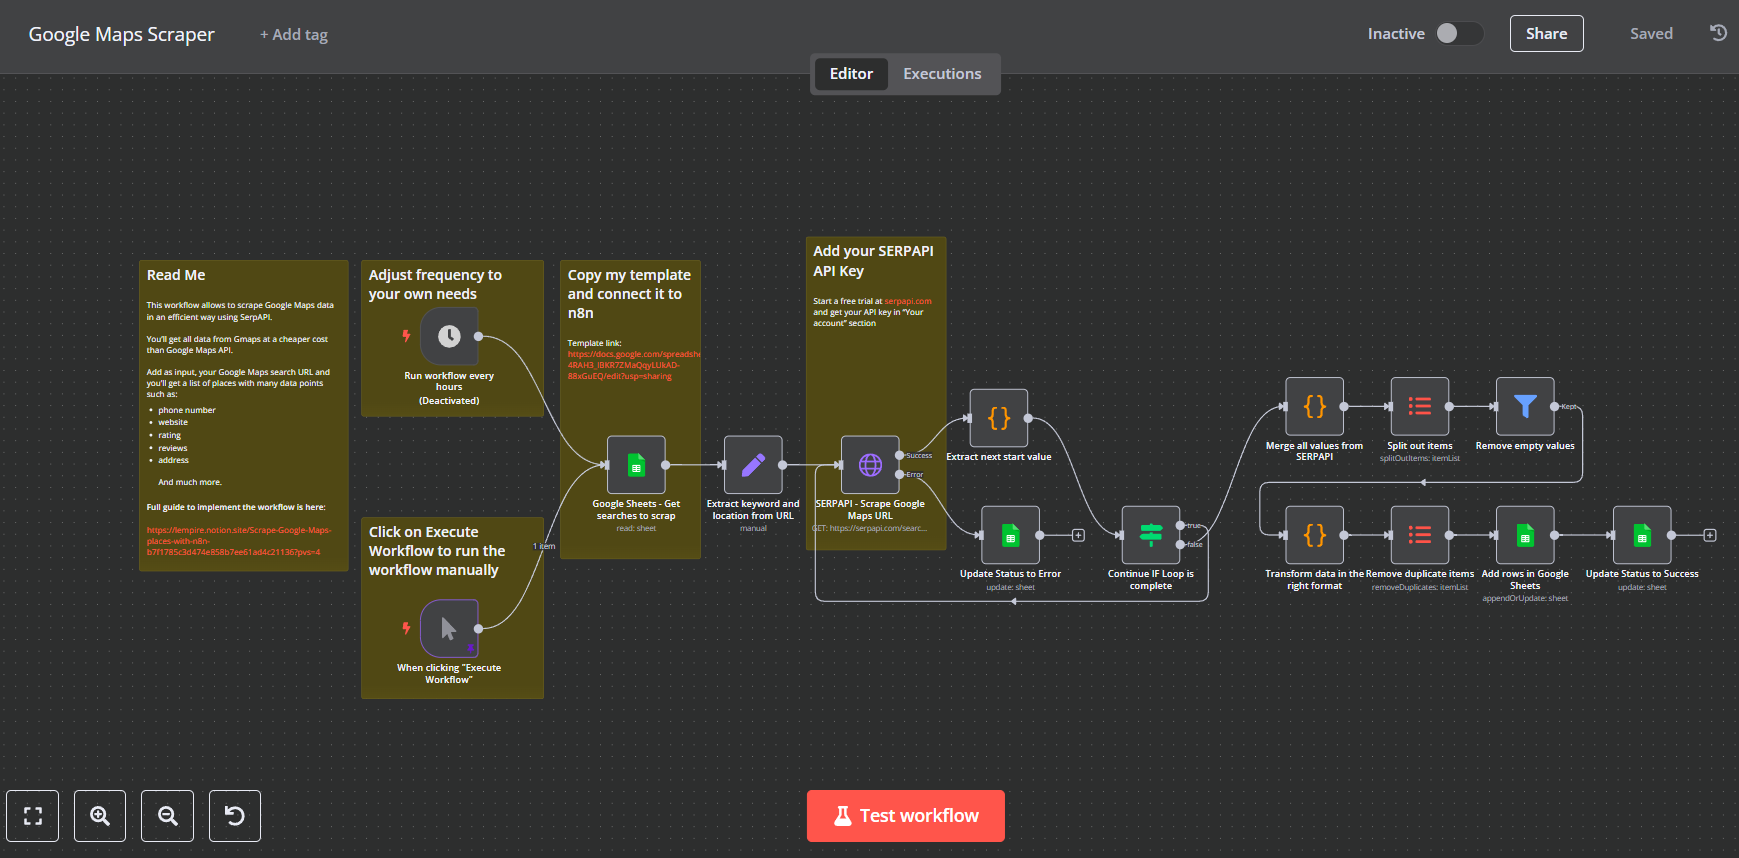
\includegraphics[width=1\textwidth]{images/2scrape01.png}
    \caption{Workflow Scrape google maps}
    \end{figure}

Đây là một workflow được thiết kế để tự động thu thập (scrape) dữ liệu từ Google Maps sử dụng SerpAPI. Workflow này được tạo trong n8n - một nền tảng tự động hóa quy trình làm việc (workflow automation platform).

\subsection{Tổng quan về Workflow}

Workflow này giúp bạn:
\begin{itemize}
  \item Thu thập thông tin về các địa điểm trên Google Maps (tên, số điện thoại, website, đánh giá, địa chỉ, v.v.)
  \item Lưu trữ dữ liệu vào Google Sheets
  \item Tự động lặp qua nhiều trang kết quả
  \item Theo dõi trạng thái của các yêu cầu scraping
\end{itemize}

\subsection{Các thành phần chính}

\begin{enumerate}
  \item \textbf{Trigger (Kích hoạt)}: Khởi chạy workflow bằng tay hoặc tự động theo lịch
  \item \textbf{API SerpAPI}: Sử dụng để truy vấn dữ liệu từ Google Maps
  \item \textbf{Google Sheets}: Lấy danh sách URL cần scrape và lưu kết quả
  \item \textbf{Code nodes}: Xử lý dữ liệu và quản lý việc phân trang
\end{enumerate}

\subsection{Hướng dẫn chi tiết từng bước}

\subsubsection{Bước 1: Chuẩn bị}

\begin{enumerate}
  \item \textbf{Tạo tài khoản SerpAPI}:
  \begin{itemize}
    \item Đăng ký tại \url{https://serpapi.com/}
    \item Lấy API key từ phần Your account
  \end{itemize}

  \item \textbf{Chuẩn bị Google Sheets}:
  \begin{itemize}
    \item Sao chép template từ link: \url{https://docs.google.com/spreadsheets/d/170osqaLBql9M-4RAH3_lBKR7ZMaQqyLUkAD-88xGuEQ/edit?usp=sharing}
    \item Sheet này có 2 tab chính:
    \begin{itemize}
      \item \textbf{Scrape Maps}: Nơi bạn thêm URL Google Maps cần scrape
      \item \textbf{Result}: Nơi lưu kết quả thu được
    \end{itemize}
  \end{itemize}
\end{enumerate}

\subsubsection{Bước 2: Thiết lập workflow trong n8n}

\begin{enumerate}
  \item \textbf{Tạo workflow mới} trong n8n

  \item \textbf{Thêm Trigger node}:
  \begin{itemize}
    \item Có 2 lựa chọn:
    \begin{itemize}
      \item ``When clicking Execute Workflow'' (chạy thủ công)
      \item ``Run workflow every hours'' (chạy tự động theo lịch)
    \end{itemize}
  \end{itemize}

  \item \textbf{Kết nối với Google Sheets}:
  \begin{itemize}
    \item Thêm node ``Google Sheets - Get searches to scrap''
    \item Kết nối với Google account của bạn
    \item Chọn document ID của sheet đã sao chép
    \item Chọn sheet tab ``Scrape Maps''
  \end{itemize}

  \item \textbf{Xử lý URL từ Google Maps}:
  \begin{itemize}
    \item Thêm node ``Extract keyword and location from URL''
    \item Node này sử dụng regular expression để trích xuất:
    \begin{itemize}
      \item Từ khóa tìm kiếm (\texttt{keyword})
      \item Tọa độ địa lý (\texttt{geo})
    \end{itemize}
  \end{itemize}

  \item \textbf{Kết nối với SerpAPI}:
  \begin{itemize}
    \item Thêm node ``SERPAPI - Scrape Google Maps URL''
    \item Cấu hình các tham số:
    \begin{itemize}
      \item \texttt{engine}: google\_maps
      \item \texttt{q}: Từ khóa đã trích xuất
      \item \texttt{ll}: Tọa độ địa lý đã trích xuất
      \item \texttt{type}: search
      \item \texttt{start}: Tham số phân trang (bắt đầu từ 0)
    \end{itemize}
    \item Thêm API key SerpAPI vào phần credentials
  \end{itemize}

  \item \textbf{Xử lý phân trang}:
  \begin{itemize}
    \item Thêm node ``Extract next start value''
    \item Node này kiểm tra nếu có trang tiếp theo và trích xuất tham số \texttt{start} để tiếp tục quá trình scraping
  \end{itemize}

  \item \textbf{Điều kiện lặp}:
  \begin{itemize}
    \item Thêm node ``Continue IF Loop is complete''
    \item Kiểm tra 2 điều kiện:
    \begin{itemize}
      \item \texttt{\$json.search\_parameters.start} <= 40 (giới hạn số trang)
      \item \texttt{\$json.serpapi\_pagination.next} không rỗng (còn trang tiếp theo)
    \end{itemize}
    \item Nếu đúng → quay lại node SERPAPI để lấy trang tiếp theo
    \item Nếu sai → tiến hành xử lý dữ liệu đã thu thập
  \end{itemize}

  \item \textbf{Xử lý dữ liệu}:
  \begin{itemize}
    \item Thêm node ``Merge all values from SERPAPI'' để gộp kết quả từ tất cả các trang
    \item Thêm node ``Split out items'' để tách từng mục riêng lẻ
    \item Thêm node ``Remove empty values'' để loại bỏ giá trị rỗng
    \item Thêm node ``Transform data in the right format'' để định dạng dữ liệu
    \item Thêm node ``Remove duplicate items'' để loại bỏ các mục trùng lặp
  \end{itemize}

  \item \textbf{Lưu kết quả vào Google Sheets}:
  \begin{itemize}
    \item Thêm node ``Add rows in Google Sheets''
    \item Kết nối với Google account
    \item Chọn document ID và sheet tab ``Result''
    \item Ánh xạ các trường dữ liệu vào các cột tương ứng
  \end{itemize}

  \item \textbf{Cập nhật trạng thái}:
  \begin{itemize}
    \item Thêm node ``Update Status to Success'' để cập nhật trạng thái thành công (tick xanh)
    \item Thêm node ``Update Status to Error'' để cập nhật trạng thái lỗi (X đỏ)
  \end{itemize}
\end{enumerate}

\subsubsection{Bước 3: Chạy và quản lý workflow}

\begin{enumerate}
  \item \textbf{Cách thêm URL Google Maps cần scrape}:
  \begin{itemize}
    \item Mở Google Sheet đã tạo
    \item Vào tab ``Scrape Maps''
    \item Thêm URL Google Maps vào cột URL, Vào GG maps nhập từ khoá về ngành bạn muốn quét, sau đó copy link 
  \end{itemize}

  \item \textbf{Chạy workflow}:
  \begin{itemize}
    \item Chọn node ``When clicking Execute Workflow'' và nhấn ``Execute Workflow''
    \item Hoặc bật node ``Run workflow every hours'' để chạy tự động
  \end{itemize}

  \item \textbf{Kiểm tra kết quả}:
  \begin{itemize}
    \item Kết quả sẽ được lưu vào tab ``Result'' của Google Sheet
    \item Trạng thái của mỗi URL sẽ được cập nhật trong tab ``Scrape Maps'':
    \begin{itemize}
      \item tick xanh: Thành công
      \item X đỏ: Lỗi
    \end{itemize}
  \end{itemize}
\end{enumerate}

\subsection{Chi tiết về xử lý dữ liệu}

\subsubsection{Node ``Extract keyword and location from URL''}
\begin{verbatim}
// Trích xuất từ khóa từ URL
{{ $json.URL.match(/\/search\/(.*?)\//)[1] }}

// Trích xuất tọa độ địa lý từ URL
{{ $json.URL.match(/(@[^\/?]+)/)[1] }}
\end{verbatim}

\subsubsection{Node ``Extract next start value''}
\begin{verbatim}
let nextUrl

if ($json && $json["serpapi_pagination"] && $json["serpapi_pagination"]["next"]) {
    nextUrl = $json["serpapi_pagination"]["next"];
    
    $input.item.json.start = nextUrl.split('&').find(param => 
        param.startsWith('start=')).split('=')[1];
}

return $input.item;
\end{verbatim}

\subsubsection{Node ``Merge all values from SERPAPI''}
\begin{verbatim}
const allData = []

let counter = 0;
do {
  try {
    const items = $items("SERPAPI - Scrape Google Maps URL", 0, counter)
                  .map(item => item.json.local_results);
    allData.push.apply(allData, items);
  } catch (error) {
    return [{json: {allData}}];  
  }

  counter++;
} while(true);
\end{verbatim}

\subsection{Dữ liệu được thu thập}

Workflow này thu thập nhiều thông tin từ mỗi địa điểm trên Google Maps, bao gồm:

\begin{itemize}
  \item \textbf{place\_id}: ID định danh duy nhất của địa điểm
  \item \textbf{title}: Tên địa điểm
  \item \textbf{phone}: Số điện thoại
  \item \textbf{website}: Trang web
  \item \textbf{rating}: Điểm đánh giá
  \item \textbf{reviews}: Số lượng đánh giá
  \item \textbf{type}: Loại địa điểm
  \item \textbf{address}: Địa chỉ
  \item \textbf{hours}: Giờ làm việc
  \item \textbf{operating\_hours}: Chi tiết giờ hoạt động
  \item \textbf{service\_options}: Các tùy chọn dịch vụ
  \item \textbf{thumbnail}: Hình thu nhỏ
  \item và nhiều thông tin khác
\end{itemize}

\subsection{Ưu điểm của workflow này}

\begin{enumerate}
  \item \textbf{Hiệu quả về chi phí}: Sử dụng SerpAPI thay vì Google Maps API chính thức (thường đắt hơn)
  \item \textbf{Tự động hóa}: Có thể chạy tự động theo lịch
  \item \textbf{Quản lý tốt}: Theo dõi trạng thái scraping của từng URL
  \item \textbf{Toàn diện}: Thu thập nhiều loại thông tin hữu ích
  \item \textbf{Chống trùng lặp}: Loại bỏ các dữ liệu trùng lặp
\end{enumerate}

\subsection{Các lưu ý quan trọng}

\begin{enumerate}
  \item \textbf{Giới hạn API}: SerpAPI có giới hạn số lượng requests trong gói miễn phí, nên theo dõi việc sử dụng
  \item \textbf{Giới hạn phân trang}: Workflow được cấu hình để dừng sau 40 kết quả (điều này có thể điều chỉnh)
  \item \textbf{Quyền Google Sheets}: Đảm bảo tài khoản Google có quyền truy cập đầy đủ vào Google Sheet
  \item \textbf{Kiểm tra định kỳ}: Kiểm tra tab ``Scrape Maps'' để xem trạng thái của các yêu cầu scraping
\end{enumerate}

\subsection{Cách điều chỉnh workflow}

\begin{enumerate}
  \item \textbf{Thay đổi giới hạn phân trang}:
  \begin{itemize}
    \item Chỉnh sửa điều kiện trong node ``Continue IF Loop is complete''
    \item Thay đổi giá trị \texttt{40} thành số trang mong muốn
  \end{itemize}

  \item \textbf{Thay đổi tần suất tự động chạy}:
  \begin{itemize}
    \item Chỉnh sửa node ``Run workflow every hours''
    \item Thay đổi tần suất từ ``hours'' thành ``days'', ``minutes'', v.v.
  \end{itemize}

  \item \textbf{Thêm trường dữ liệu}:
  \begin{itemize}
    \item Chỉnh sửa ánh xạ trong node ``Add rows in Google Sheets''
    \item Thêm cột mới vào Google Sheet
  \end{itemize}
\end{enumerate}

Với việc thiết lập đúng cách, workflow này sẽ giúp bạn thu thập dữ liệu từ Google Maps một cách hiệu quả và tự động, phù hợp cho nhiều mục đích như nghiên cứu thị trường, tìm kiếm khách hàng tiềm năng, hoặc phân tích cạnh tranh.

\clearpage
%---------------------------------------------------------------------
\section{\textbf{Dự án 2: Tạo chatbot theo dõi thu chi bằng n8n qua Telegram }}

\href{https://drive.google.com/drive/folders/1tumFktBej5fgHsKSuYDtnL2V0W5OI9nk?usp=sharing}{\textbf{\underline {Link tải workflow}}}

\begin{figure}[h]
    \centering
    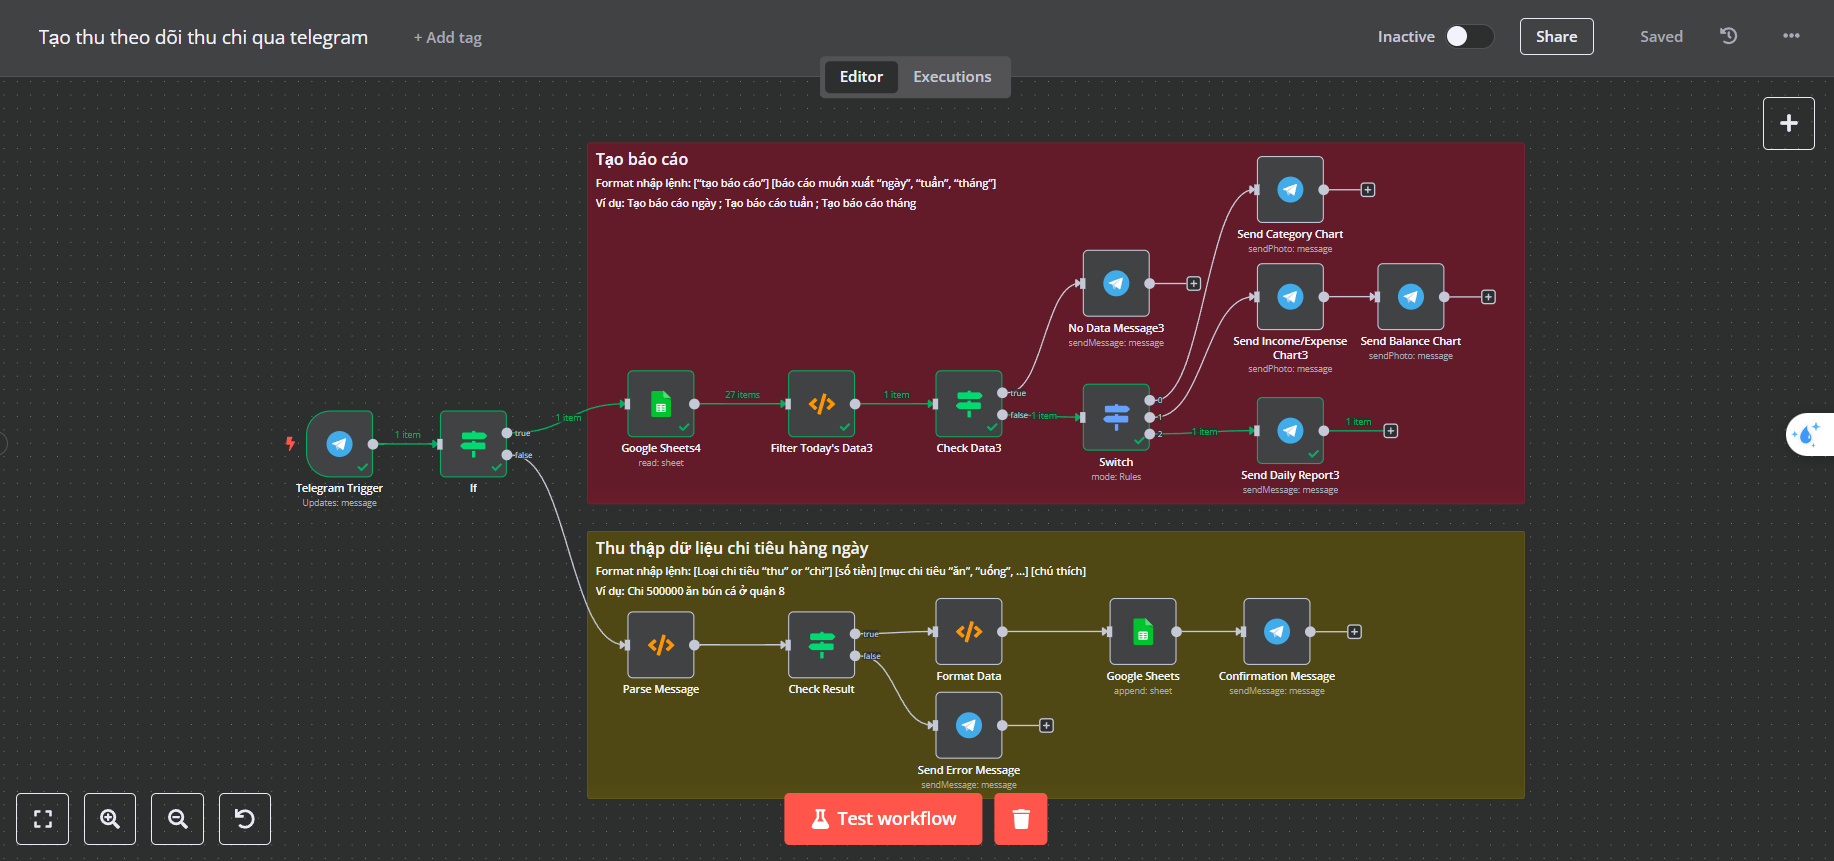
\includegraphics[width=1\textwidth]{images/3thuchi01.png}
    \caption{Workflow theo dõi thu chi}
    
\end{figure}

Đây là một workflow phức tạp nhưng rất hữu ích được xây dựng trên nền tảng n8n để theo dõi tài chính cá nhân thông qua một bot Telegram. Bài viết sẽ phân tích chi tiết các thành phần chính, ưu điểm và cách thiết lập.

\subsection{Tổng quan về workflow}

Workflow này tạo ra một bot Telegram cho phép người dùng:
\begin{enumerate}
    \item Ghi lại các khoản thu chi hàng ngày một cách nhanh chóng
    \item Tạo báo cáo tài chính theo ngày, tuần, tháng với biểu đồ trực quan
    \item Lưu trữ dữ liệu vào Google Sheets để dễ dàng theo dõi và phân tích
\end{enumerate}

\subsection{Các thành phần chính}

\subsubsection{Thu thập dữ liệu từ người dùng}
Bot nhận tin nhắn từ người dùng theo các định dạng:
\begin{itemize}
    \item Nhập khoản chi tiêu: \texttt{[thu/chi] [số tiền] [danh mục] [ghi chú]}
    \begin{itemize}
        \item Ví dụ: \texttt{Chi 500000 ăn bún cá ở quận 8}
    \end{itemize}
    \item Yêu cầu báo cáo: \texttt{Tạo báo cáo [ngày/tuần/tháng]}
    \begin{itemize}
        \item Ví dụ: \texttt{Tạo báo cáo tuần}
    \end{itemize}
\end{itemize}

\subsubsection{Lưu trữ dữ liệu}
\begin{itemize}
    \item Sử dụng Google Sheets làm cơ sở dữ liệu
    \item Mỗi giao dịch được ghi lại với các thông tin: ngày tháng, loại (thu/chi), số tiền, danh mục, ghi chú
\end{itemize}

\subsubsection{Phân tích dữ liệu}
\begin{itemize}
    \item Node Function xử lý phức tạp để tính toán tổng thu, tổng chi và số dư
    \item Phân loại chi tiêu theo danh mục
    \item So sánh với tuần trước để thấy xu hướng
    \item Đưa ra gợi ý tiết kiệm
\end{itemize}

\subsubsection{Tạo báo cáo trực quan}
\begin{itemize}
    \item Sử dụng QuickChart.io để tạo 3 loại biểu đồ:
    \begin{itemize}
        \item Biểu đồ cột thể hiện thu/chi của 4 tuần gần nhất
        \item Biểu đồ đường thể hiện biến động số dư
        \item Biểu đồ tròn phân loại chi tiêu theo danh mục
    \end{itemize}
\end{itemize}

\subsection{Luồng hoạt động}

\begin{enumerate}
    \item \textbf{Nhận tin nhắn từ Telegram}: Node Telegram Trigger bắt tin nhắn từ người dùng
    \item \textbf{Phân loại yêu cầu}: If node kiểm tra xem người dùng muốn nhập giao dịch hay tạo báo cáo
    \item \textbf{Xử lý giao dịch mới}:
    \begin{itemize}
        \item Parse Message phân tích tin nhắn của người dùng
        \item Format Data chuẩn hóa dữ liệu
        \item Google Sheets lưu dữ liệu vào bảng tính
        \item Confirmation Message gửi xác nhận đã lưu giao dịch
    \end{itemize}
    \item \textbf{Tạo báo cáo}:
    \begin{itemize}
        \item Google Sheets4 lấy dữ liệu từ bảng tính
        \item Filter Today's Data3 xử lý và phân tích dữ liệu
        \item Check Data3 kiểm tra xem có dữ liệu không
        \item Switch phân loại loại báo cáo (ngày/tuần/tháng)
        \item Các node Send gửi báo cáo và biểu đồ trực quan
    \end{itemize}
\end{enumerate}

\subsection{Ưu điểm của workflow}

\begin{enumerate}
    \item \textbf{Đơn giản hóa việc theo dõi tài chính}: Nhập giao dịch nhanh chóng qua Telegram mà không cần mở ứng dụng phức tạp
    \item \textbf{Tự động hóa phân tích}: Tự động tính toán, phân loại và so sánh dữ liệu
    \item \textbf{Báo cáo trực quan}: Biểu đồ giúp dễ dàng nắm bắt tình hình tài chính
    \item \textbf{Dễ tiếp cận}: Sử dụng Telegram - ứng dụng nhắn tin phổ biến làm giao diện
    \item \textbf{Lưu trữ an toàn}: Dữ liệu được lưu trong Google Sheets, dễ dàng truy cập và sao lưu
    \item \textbf{Đa ngôn ngữ}: Workflow hỗ trợ tiếng Việt, dễ dàng mở rộng cho các ngôn ngữ khác
\end{enumerate}

\subsection{Hướng dẫn thiết lập cho người mới}

\subsubsection{Bước 1: Chuẩn bị tài khoản và công cụ}
\begin{itemize}
    \item Đăng ký tài khoản \href{https://n8n.io}{n8n}
    \item Tạo bot Telegram thông qua \href{https://t.me/botfather}{BotFather}
    
    \begin{figure}[H]
    \centering
    
\includegraphics[width=1\textwidth]{images/3thuchi02.png}
    \caption{Tạo token để truy cập HTTP API telegram}
    \end{figure}
    \begin{figure}[H]
    \centering
    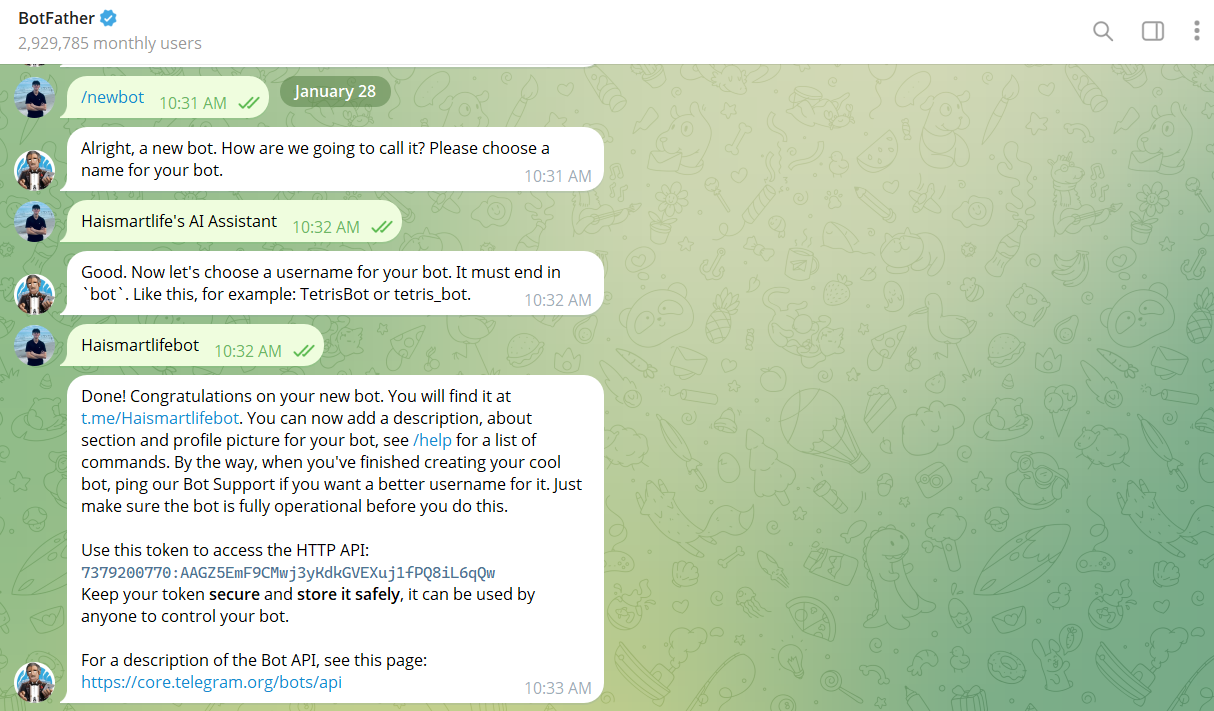
\includegraphics[width=1\textwidth]{images/3thuchi03.png}
    \caption{Tạo token để truy cập HTTP API telegram}
    \end{figure}

- Sau khi Tạo token để truy cập HTTP API telegram, chúng ta sẽ được dãi token như hình trên. \\

- Tạo credential telegram: Nhập dải token vào Access Token, và base URL \texttt{https://api.telegram.org}

    
    \begin{figure}[H]
    \centering
    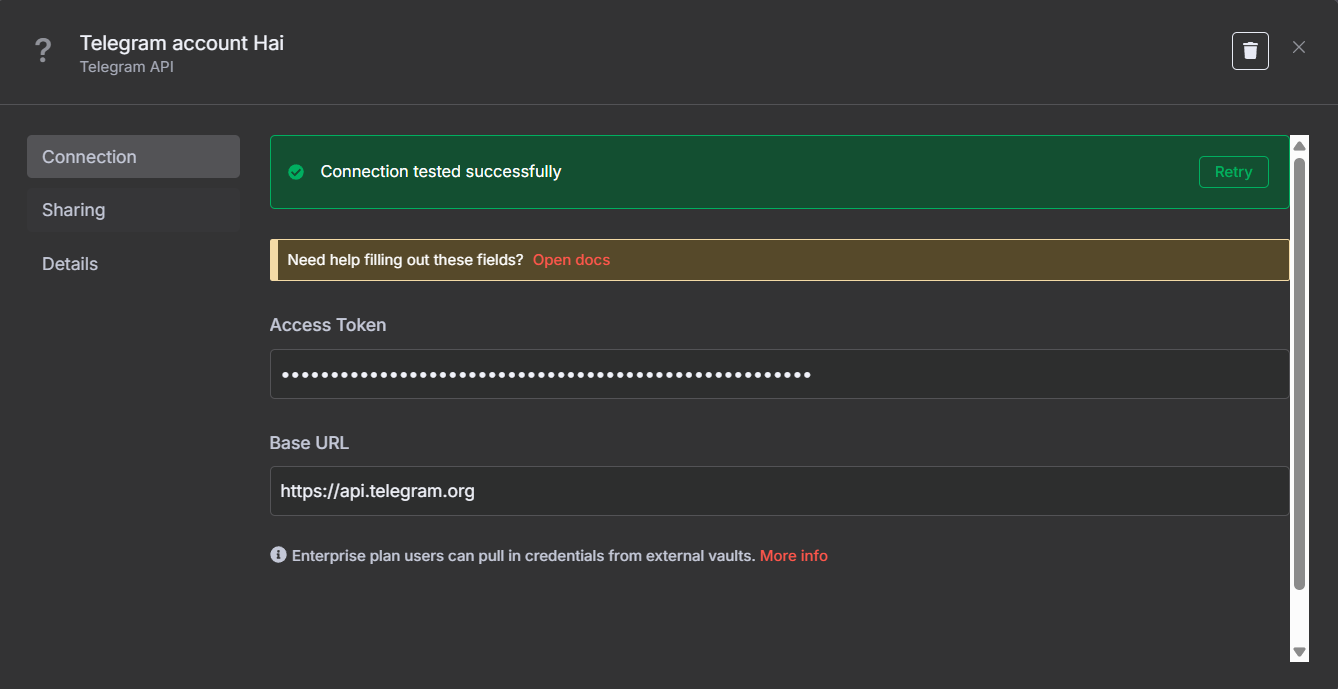
\includegraphics[width=1\textwidth]{images/3thuchi04.png}
    \caption{Tạo Credential telegram}
    \end{figure}
    
    \item Chuẩn bị một Google Sheet với các cột: date, type, amount, category, note, timestamp
    \begin{figure}[H]
    \centering
    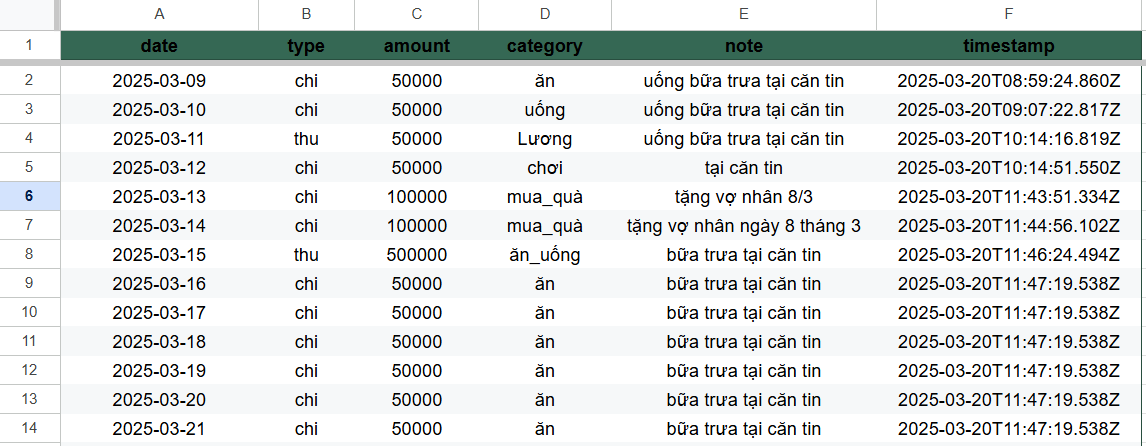
\includegraphics[width=1\textwidth]{images/3thuchi05.png}
    \caption{Form Google sheet lưu trữ thông tin chi tiêu}
    \end{figure}
    
\end{itemize}

- \textbf{\underline{Cài đặt Credeential Google sheet.}}\\
    \begin{figure}[H]
    \centering
    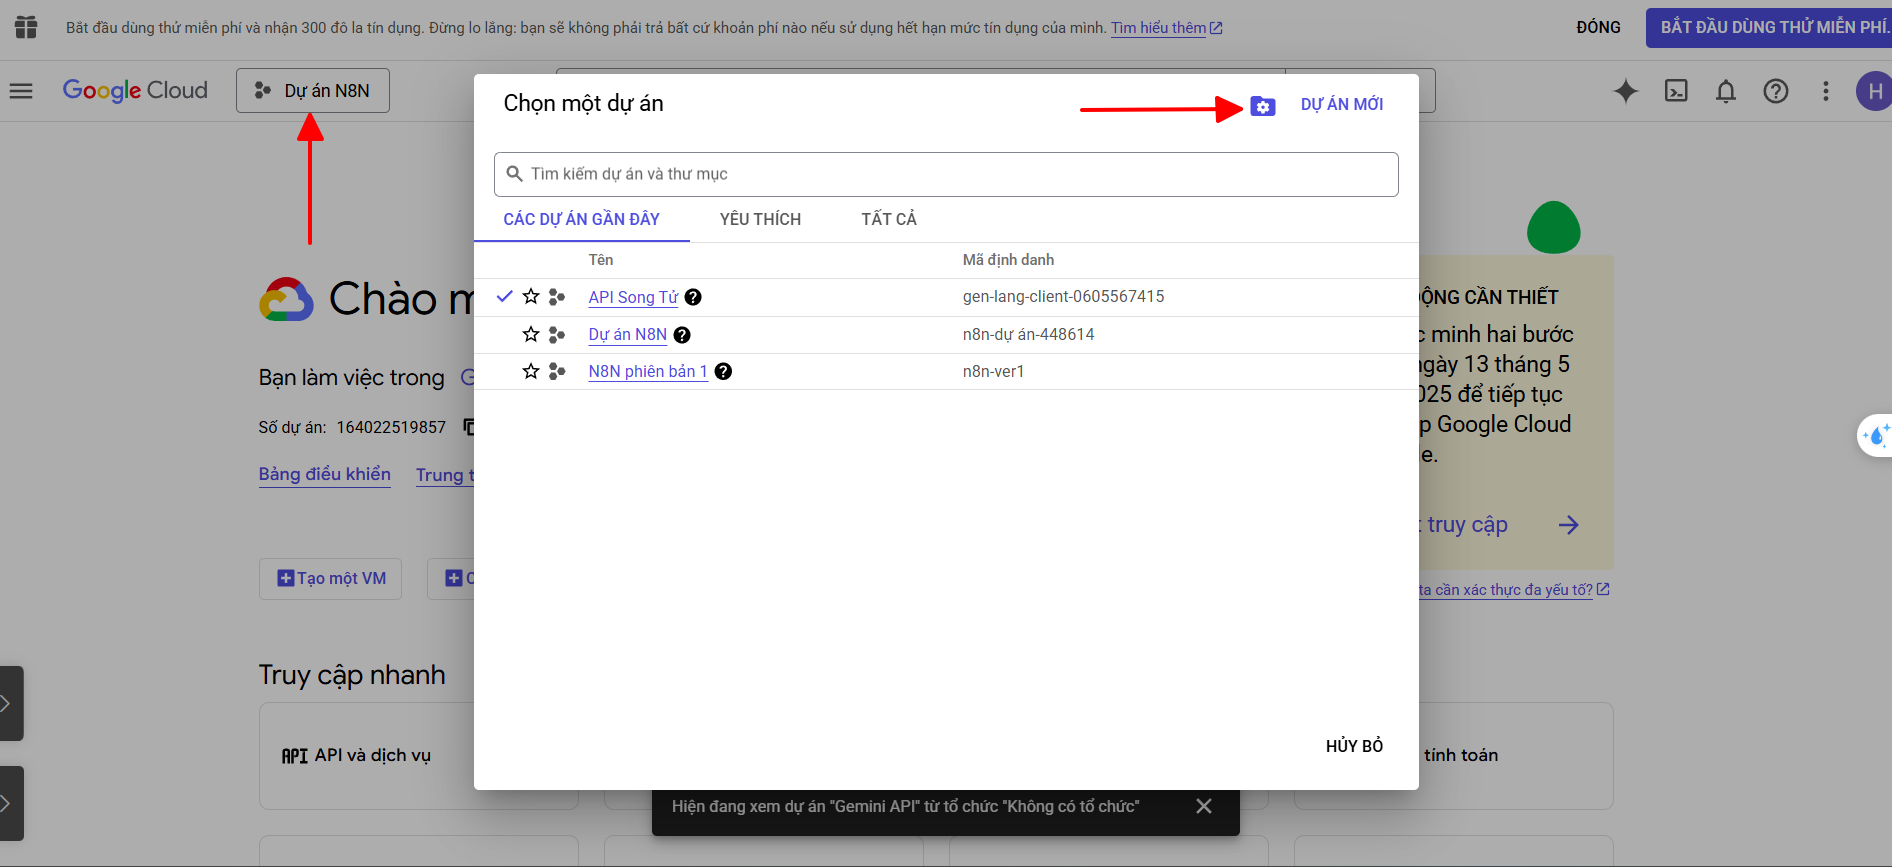
\includegraphics[width=1\textwidth]{images/3thuchi06.png}
    \caption{Tạo dự án Google Cloud Console}
    \end{figure}
$\longrightarrow$ Đăng nhập vào \url{https://console.cloud.google.com/} $\longrightarrow$ Tạo dự án mới
 
    \begin{figure}[H]
    \centering
    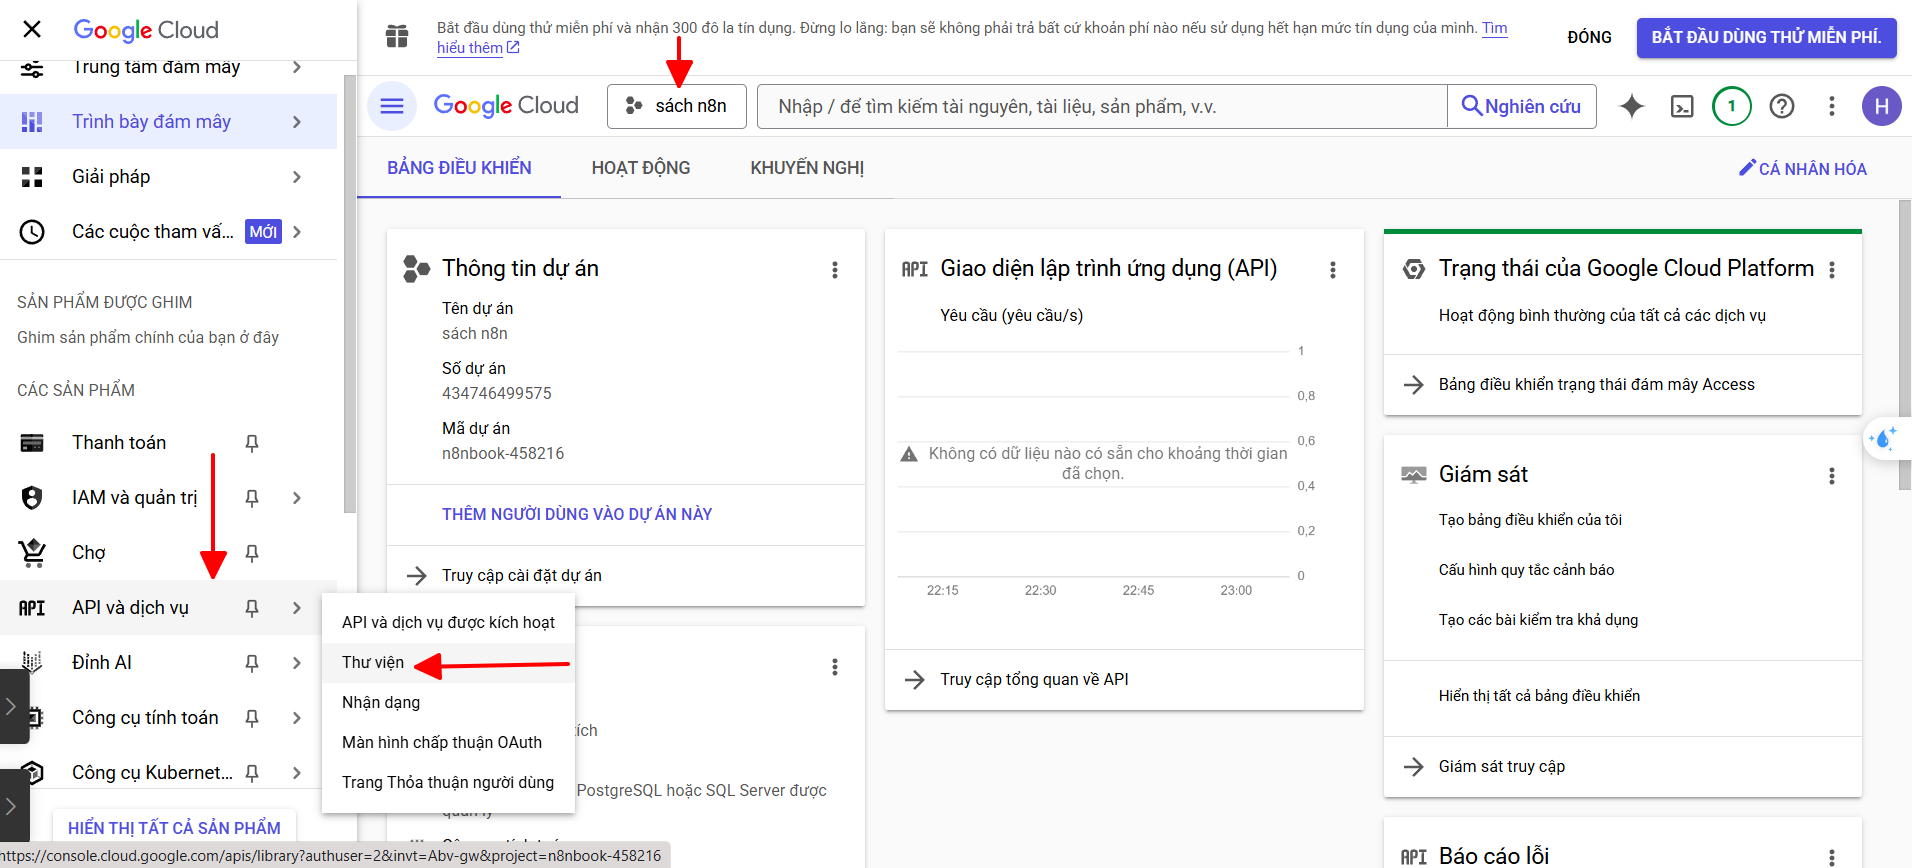
\includegraphics[width=1\textwidth]{images/3thuchi07.png}
    \caption{Enable APIs}
    \end{figure}

    \begin{figure}[H]
    \centering
    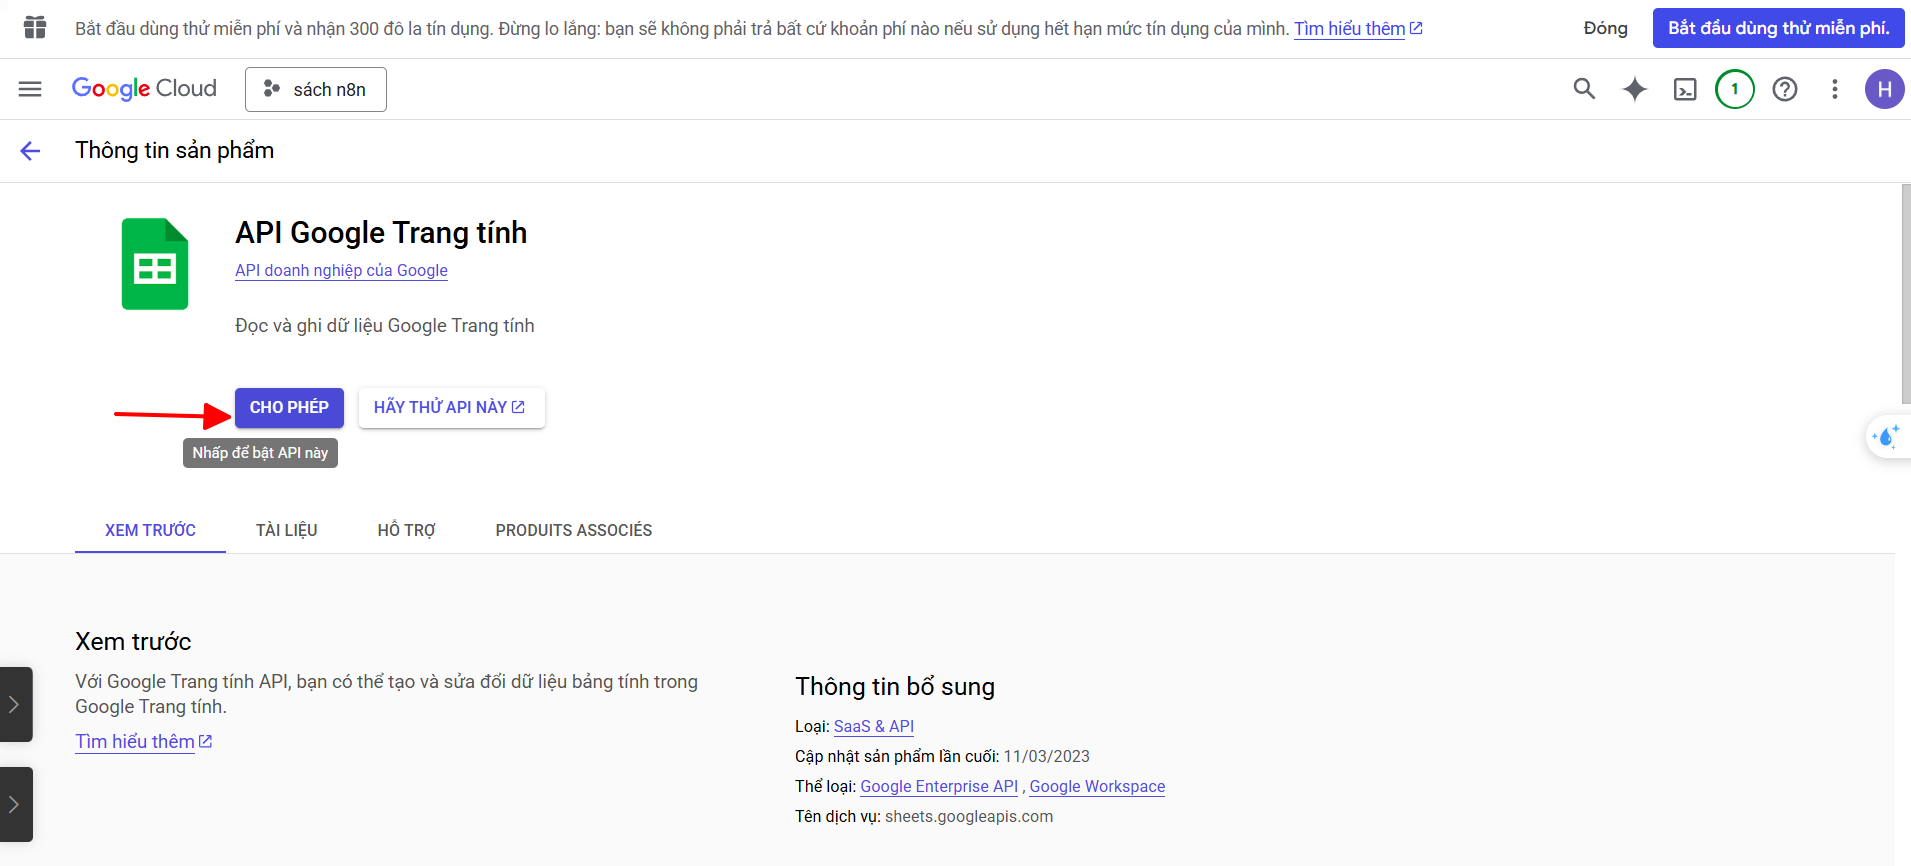
\includegraphics[width=1\textwidth]{images/3thuchi08.png}
    \caption{Enable APIs}
    \end{figure}
$\longrightarrow$ Chọn đúng tên dự án vừa tạo $\longrightarrow$ truy cập APIs and Services $>$ Library $\longrightarrow$ bật enable cho ứng dụng google mà bạn muốn phân quyền cho n8n truy cập.
    
    \begin{figure}[H]
    \centering
    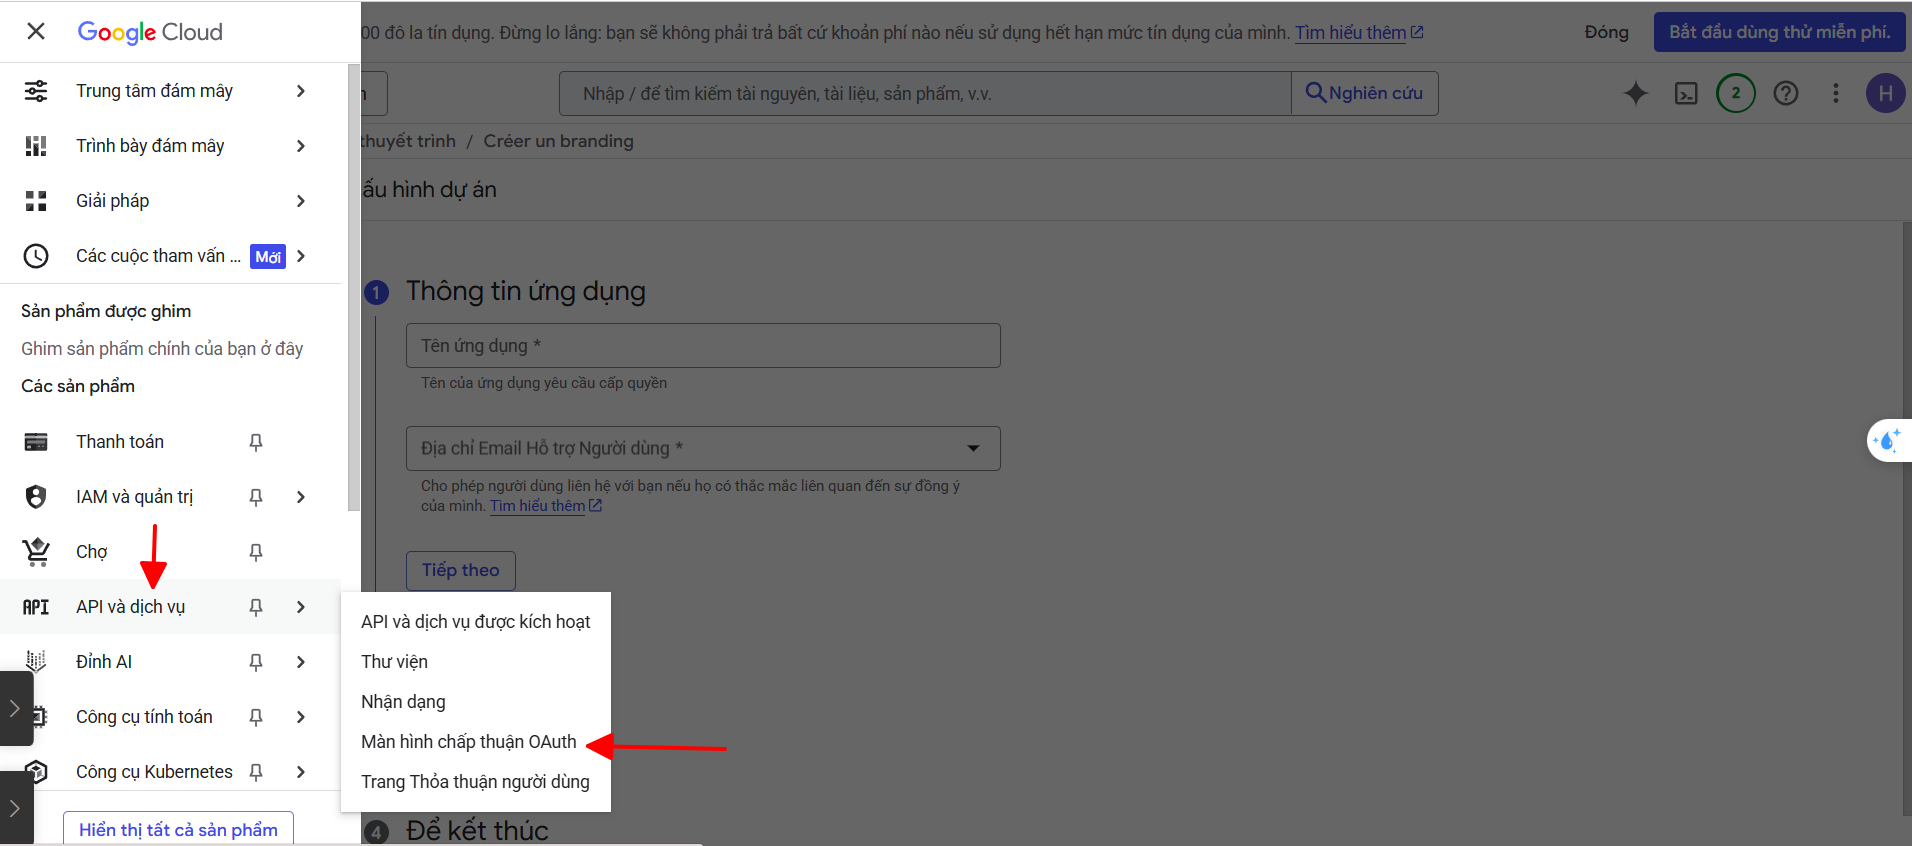
\includegraphics[width=1\textwidth]{images/3thuchi09.png}
    \caption{Configure your OAuth consent screen}
    \end{figure}

    \begin{figure}[H]
    \centering
    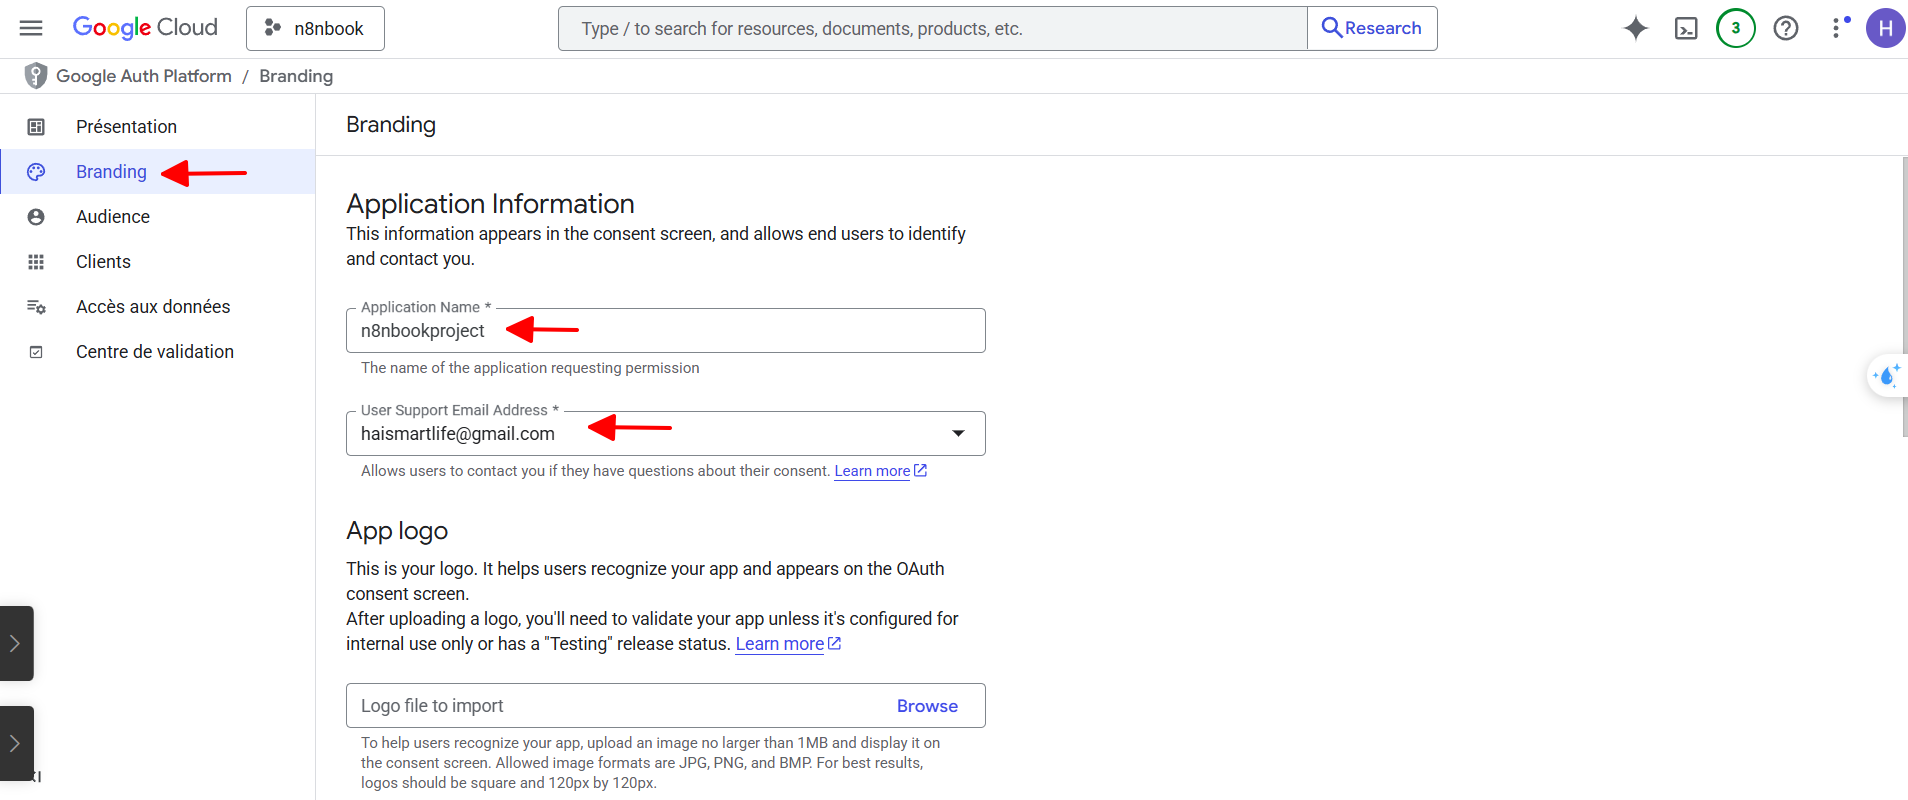
\includegraphics[width=1\textwidth]{images/3thuchi14.png}
    \caption{Configure your OAuth consent screen}
    \end{figure}

    \begin{figure}[H]
    \centering
    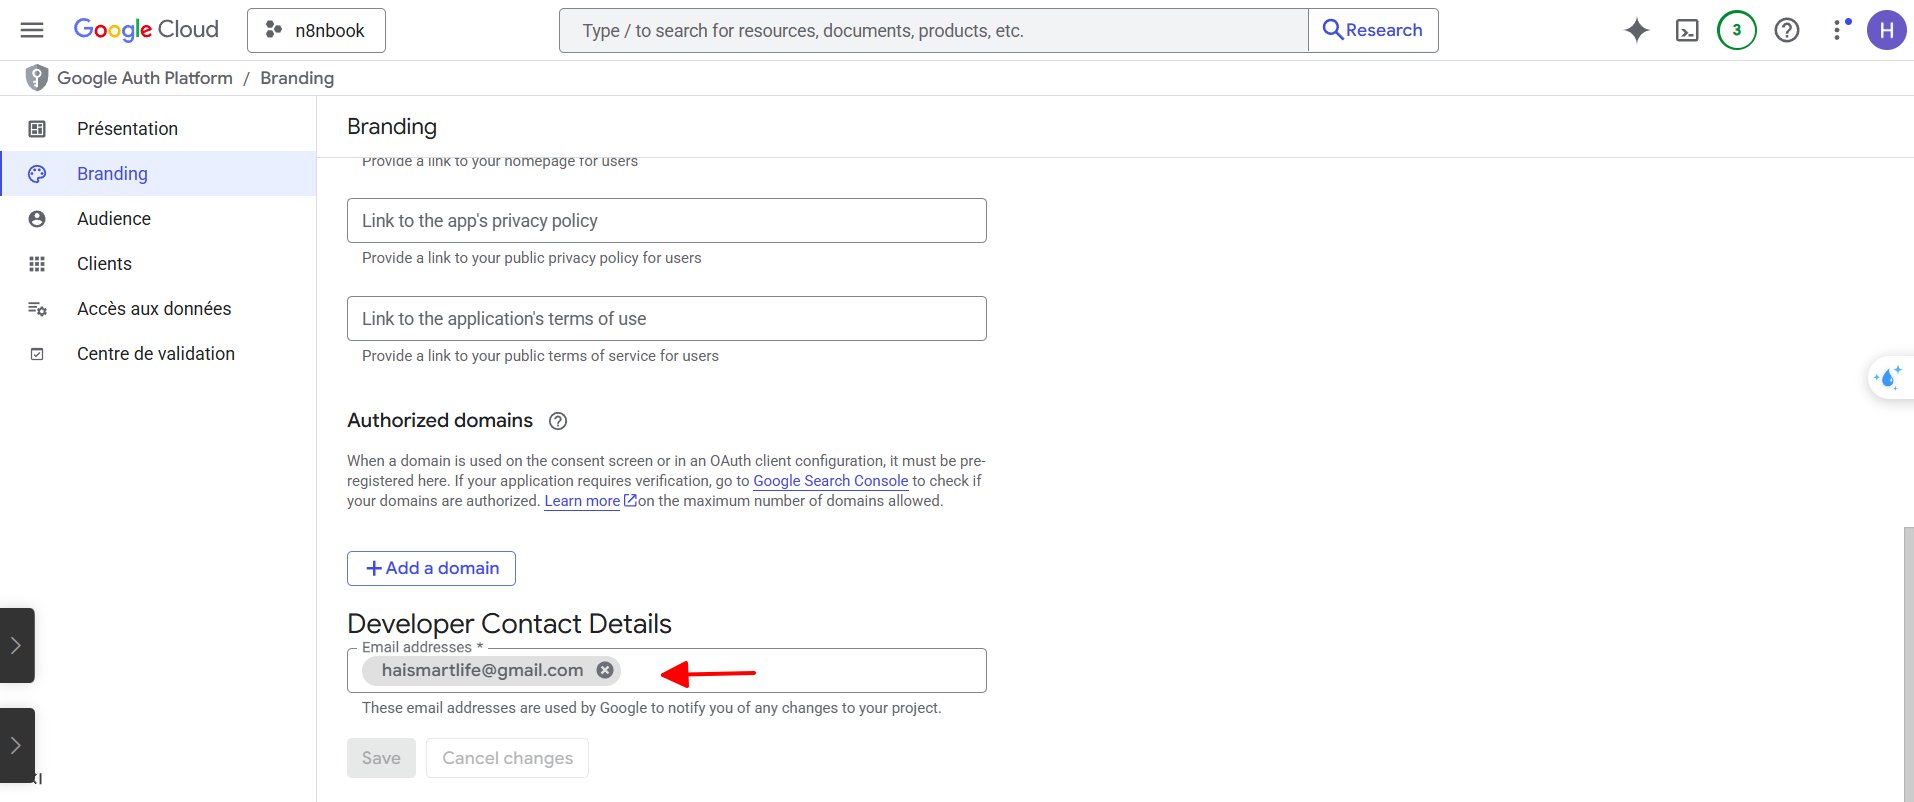
\includegraphics[width=1\textwidth]{images/3thuchi16.png}
    \caption{Configure your OAuth consent screen}
    \end{figure}
    
    \begin{figure}[H]
    \centering
    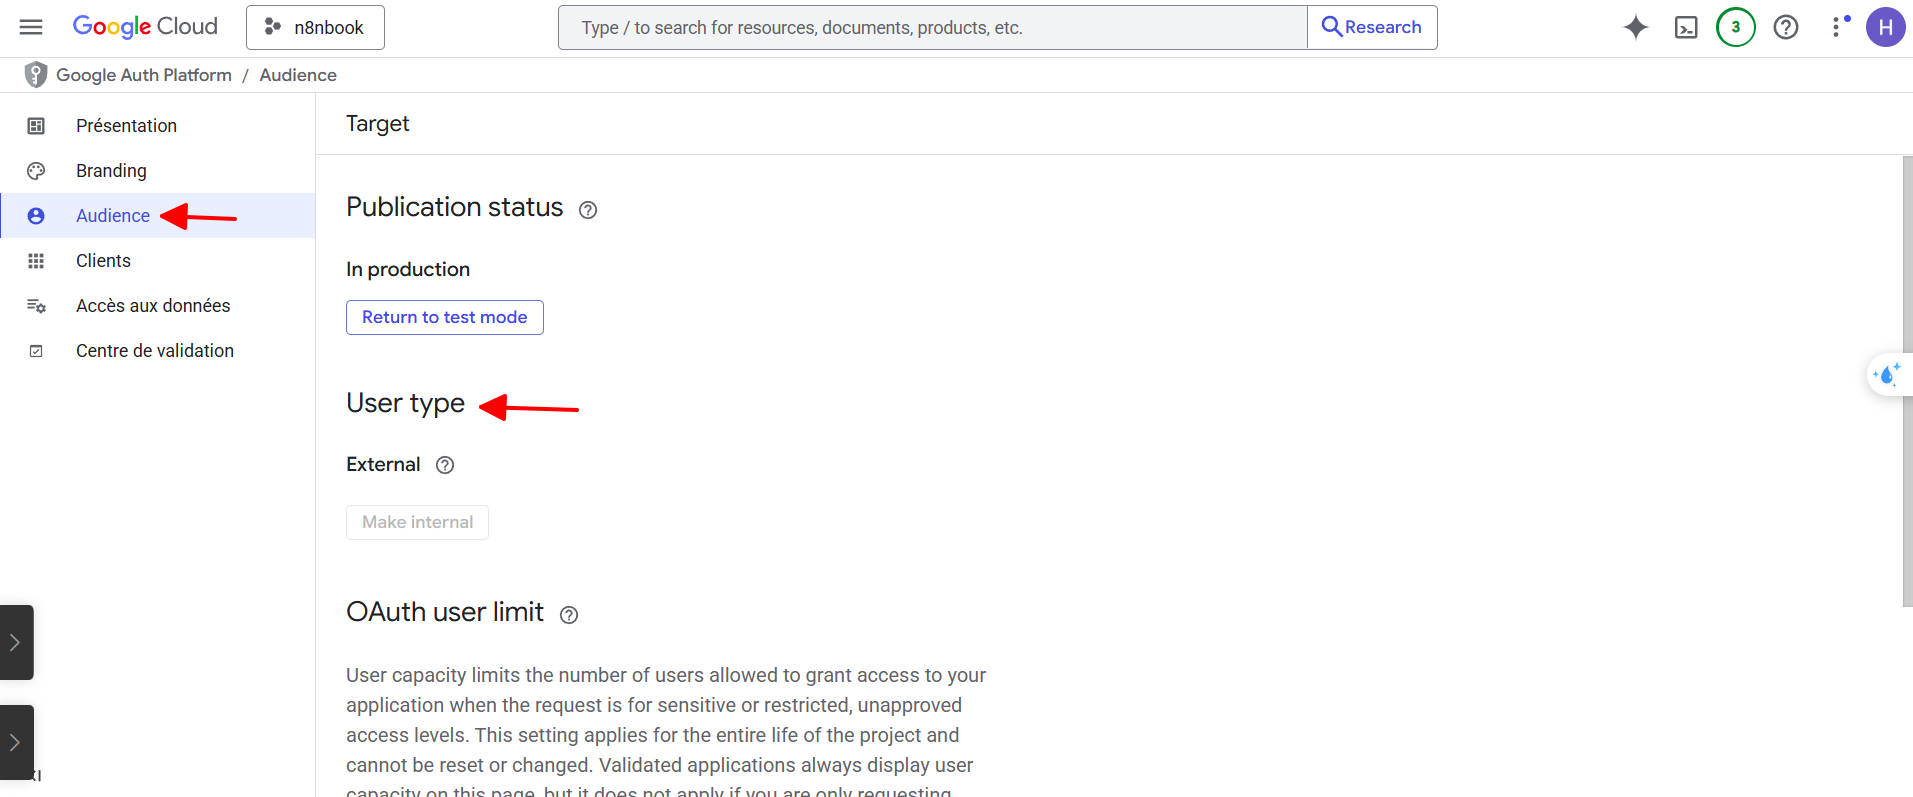
\includegraphics[width=1\textwidth]{images/3thuchi17.png}
    \caption{Configure your OAuth consent screen}
    \end{figure}
    
$\longrightarrow$ Thiết lập OAuth consent screen như hình bên trên.
    
    \begin{figure}[H]
    \centering
    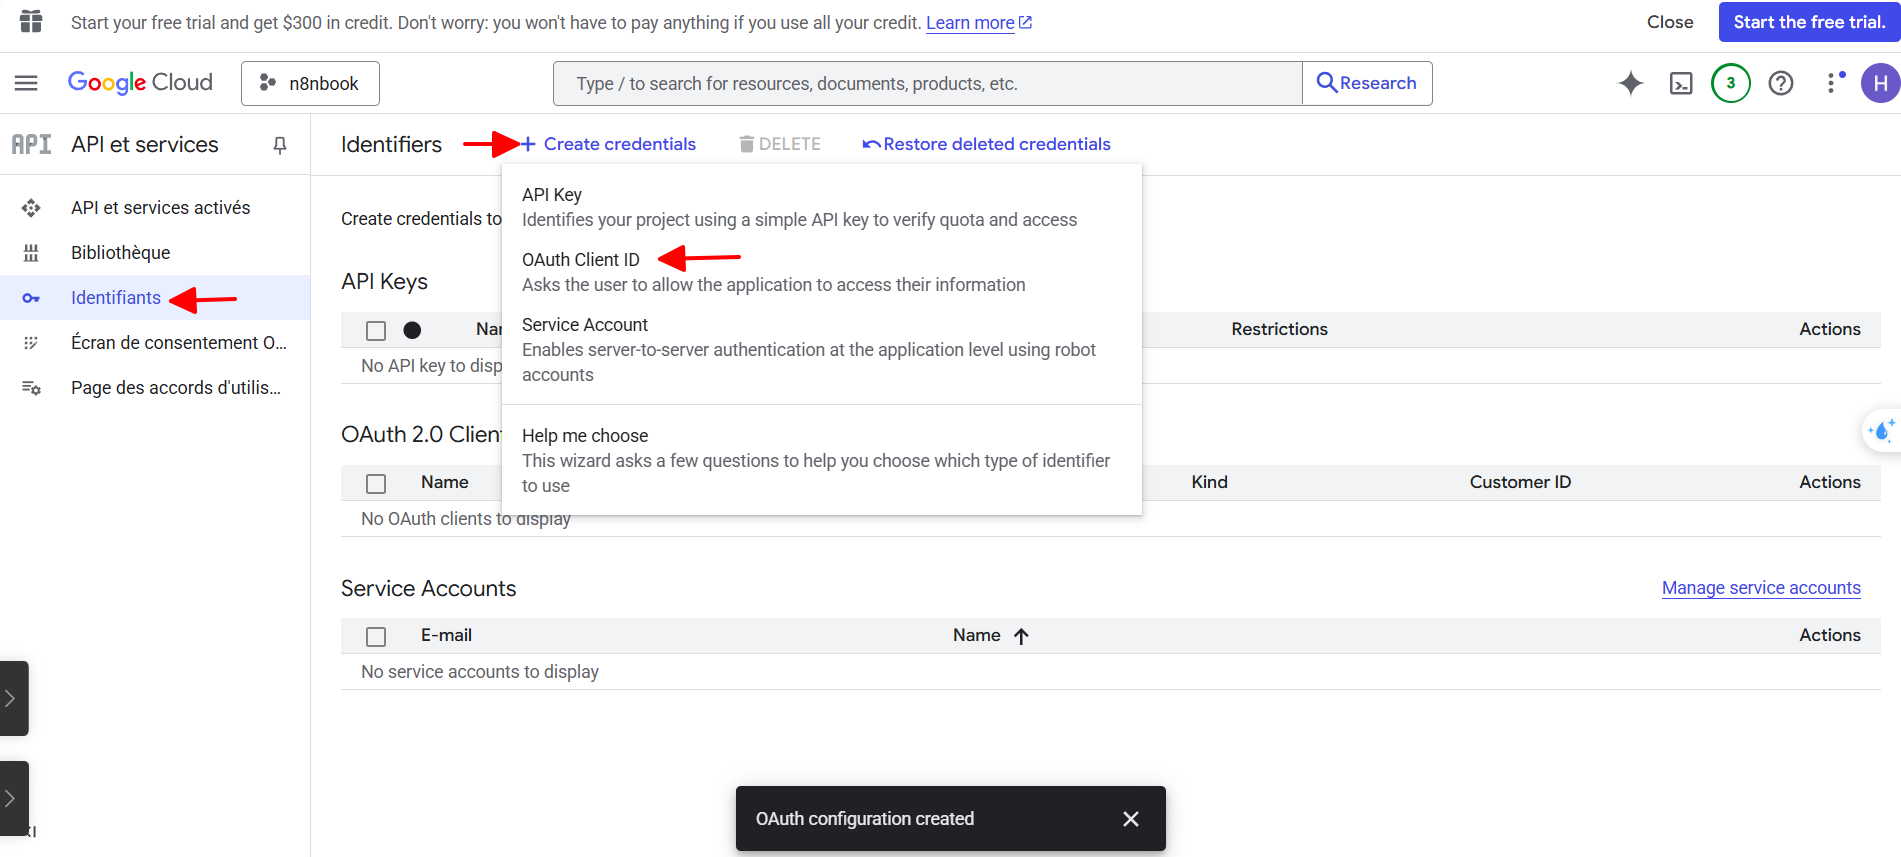
\includegraphics[width=1\textwidth]{images/3thuchi10.png}
    \caption{Create your Google OAuth client credentials}
    \end{figure}
    
$\longrightarrow$ Tìm dấu 3 gạch $\longrightarrow$ API and services $\longrightarrow$ Identifiers $\longrightarrow$ Nhấn vào Create credentials $\longrightarrow$ Oauth client ID $\longrightarrow$ chọn Web application $\longrightarrow$ đặt tên $\longrightarrow$ Allowed redirect URIs: nhập Url trong mục OAuth Redirect URL của n8n

    
    \begin{figure}[H]
    \centering
    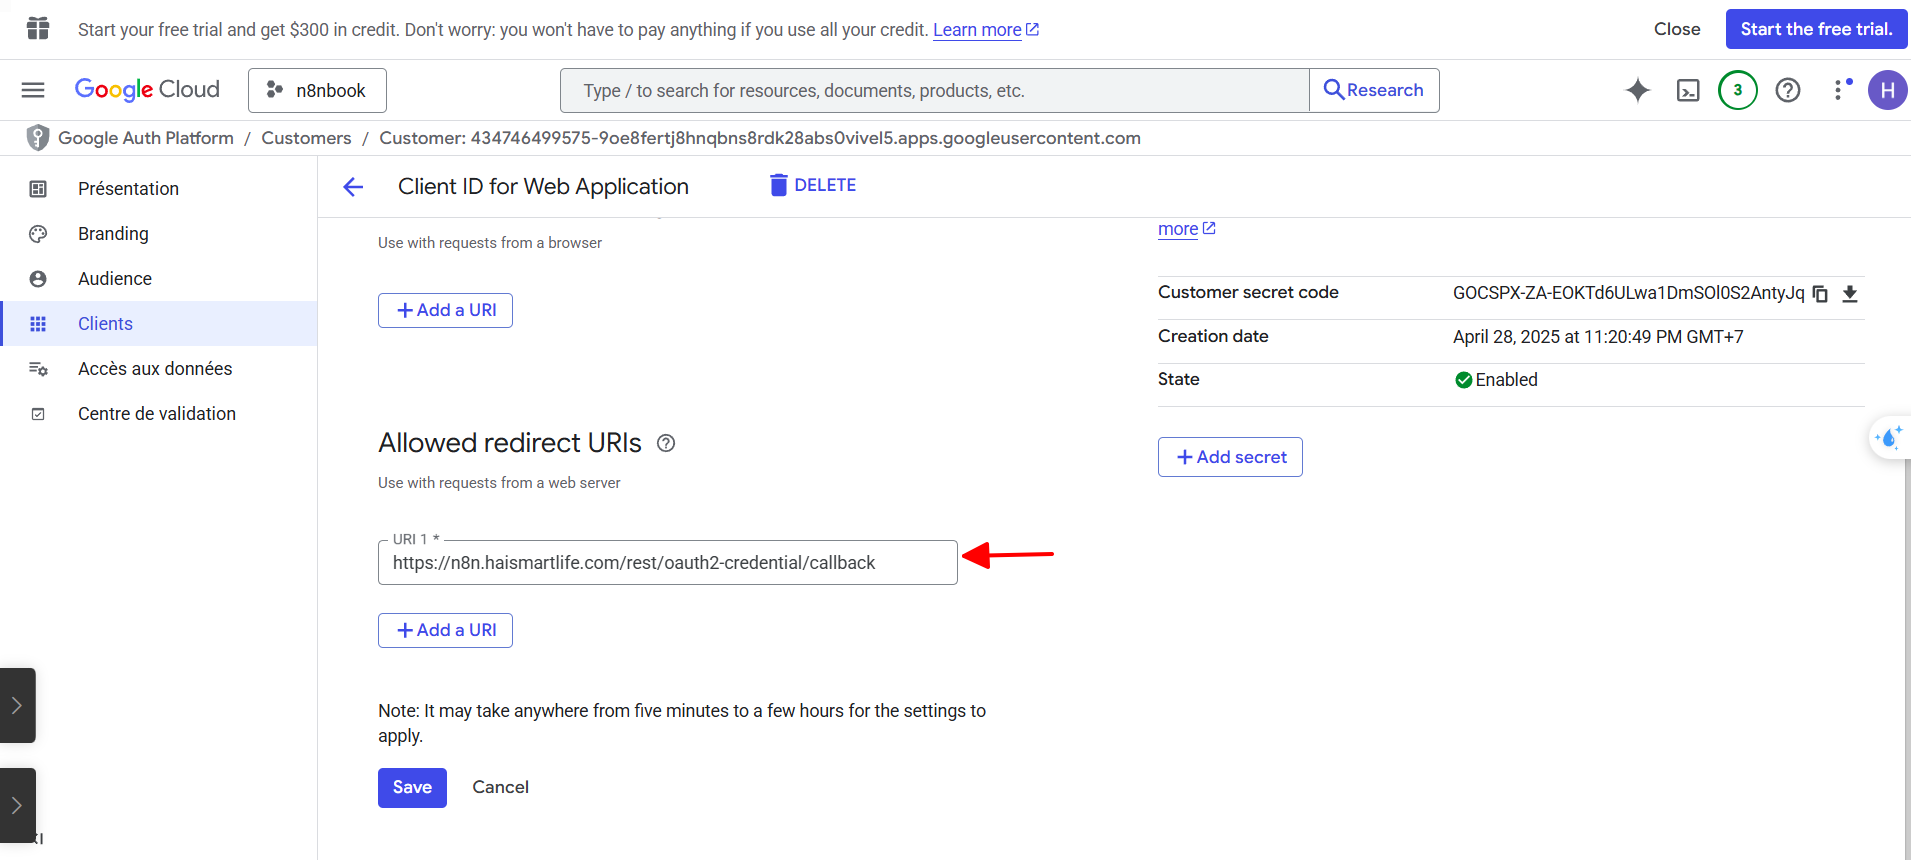
\includegraphics[width=1\textwidth]{images/3thuchi11.png}
    \caption{Create your Google OAuth client credentials}
    \end{figure}


    








\textbf{OAuth Redirect URL:} \\
\texttt{https://n8n.haismartlife.com/rest/oauth2-credential/callback}\\
$\longrightarrow$ Cho phép URL này truy cập vào ứng dụng google.\\
\textbf{Grant Type:} Authorization Code\\
\textbf{Authorization URL:}\\
\texttt{https://accounts.google.com/o/oauth2/v2/auth}\\
\textbf{Access Token URL:}\\
\texttt{https://oauth2.googleapis.com/token}\\
\textbf{Client ID:} \\
\verb|434746499575-9oe8fertj8hnqbns8rdk28abs0vivel5.apps.....|\\
$\longrightarrow$ Lấy từ OAuth 2.0 Client IDs tạo ở trên\\
\textbf{Client Secret:}\\
$\longrightarrow$ Lấy từ OAuth 2.0 Client IDs tạo ở trên
    \begin{figure}[H]
    \centering
    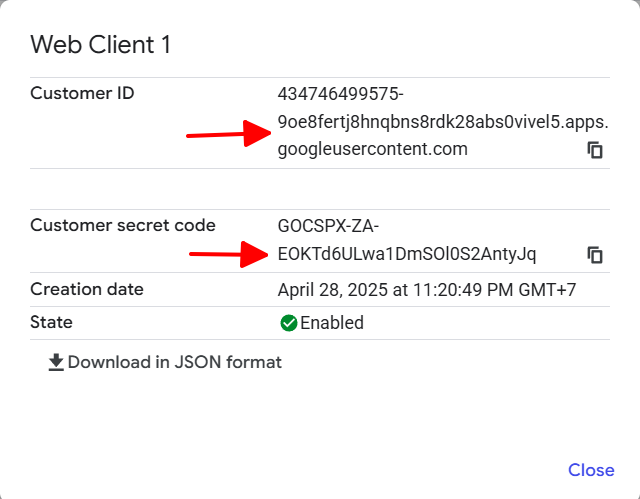
\includegraphics[width=1\textwidth]{images/3thuchi12.png}
    \caption{Tạo Credential telegram}
    \end{figure}
\textbf{Auth URI Query Parameters:}\\
\verb|access_type=offline&prompt=consent|
    \begin{figure}[H]
    \centering
    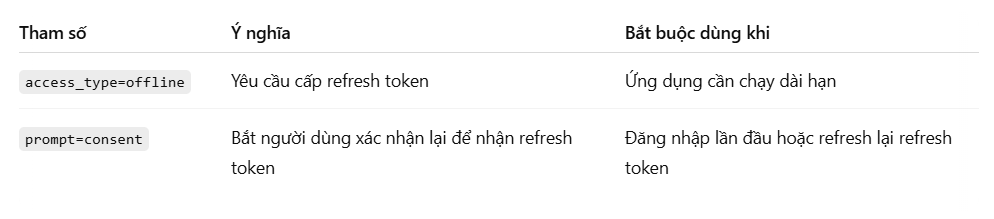
\includegraphics[width=1\textwidth]{images/3thuchi15.png}
    \caption{Tạo Credential telegram}
    \end{figure}
\textbf{Authentication:} Header\\




\subsubsection{Bước 2: Cấu hình webhook và kết nối API}
\begin{enumerate}
    \item Cài đặt credentials cho Telegram API trong n8n
    \item Cấu hình OAuth cho Google Sheets
    \item Thiết lập webhook cho Telegram Trigger
\end{enumerate}

\subsubsection{Bước 3: Tạo cấu trúc workflow}
\begin{enumerate}
    \item Bắt đầu với Telegram Trigger
    \item Thêm If node để phân loại yêu cầu
    \item Tạo nhánh xử lý nhập giao dịch
    \item Tạo nhánh tạo báo cáo
\end{enumerate}

\subsubsection{Bước 4: Cấu hình chi tiết cho từng node}
\begin{enumerate}
    \item \textbf{Parse Message}: Copy code JavaScript từ workflow mẫu để xử lý tin nhắn
    \item \textbf{Filter Today's Data3}: Copy code để phân tích và tạo biểu đồ  
    \item \textbf{Google Sheets}: Cấu hình kết nối với bảng tính của bạn
    \item \textbf{Send nodes}: Điều chỉnh định dạng tin nhắn và caption cho phù hợp
\end{enumerate}

\subsubsection{Bước 5: Kiểm tra và tối ưu}
\begin{enumerate}
    \item Chạy thử workflow với các loại tin nhắn khác nhau
    \item Kiểm tra xem dữ liệu có được lưu chính xác không
    \item Điều chỉnh các định dạng báo cáo và biểu đồ theo nhu cầu
\end{enumerate}

\subsection{Khả năng mở rộng}

Workflow này có thể được mở rộng với các tính năng:
\begin{enumerate}
    \item Thêm báo cáo theo quý/năm
    \item Tạo hệ thống ngân sách và cảnh báo khi vượt quá ngân sách
    \item Thêm chức năng xuất báo cáo dưới dạng PDF
    \item Thêm nhắc nhở thanh toán định kỳ
    \item Tích hợp với các API tài chính để tự động cập nhật giao dịch
\end{enumerate}

\subsection{Kết luận}

Với workflow này, việc theo dõi tài chính cá nhân trở nên đơn giản và trực quan hơn, giúp người dùng dễ dàng nắm bắt tình hình tài chính và đưa ra các quyết định tài chính thông minh hơn. Đây là một ví dụ điển hình về cách n8n có thể được sử dụng để tự động hóa và tối ưu các tác vụ trong cuộc sống hàng ngày mà không cần đến kỹ năng lập trình phức tạp.

\clearpage
%----------------------------------------------------------------
\section{\textbf{Dự án 3: Tạo trợ lý ảo bằng Telegram }}

\href{https://drive.google.com/drive/folders/1-qVA3yQnfIx70DsZKdPAGYQcr8WftkGJ?usp=sharing}{\textbf{\underline {Link tải workflow}}}

    \begin{figure}[H]
    \centering
    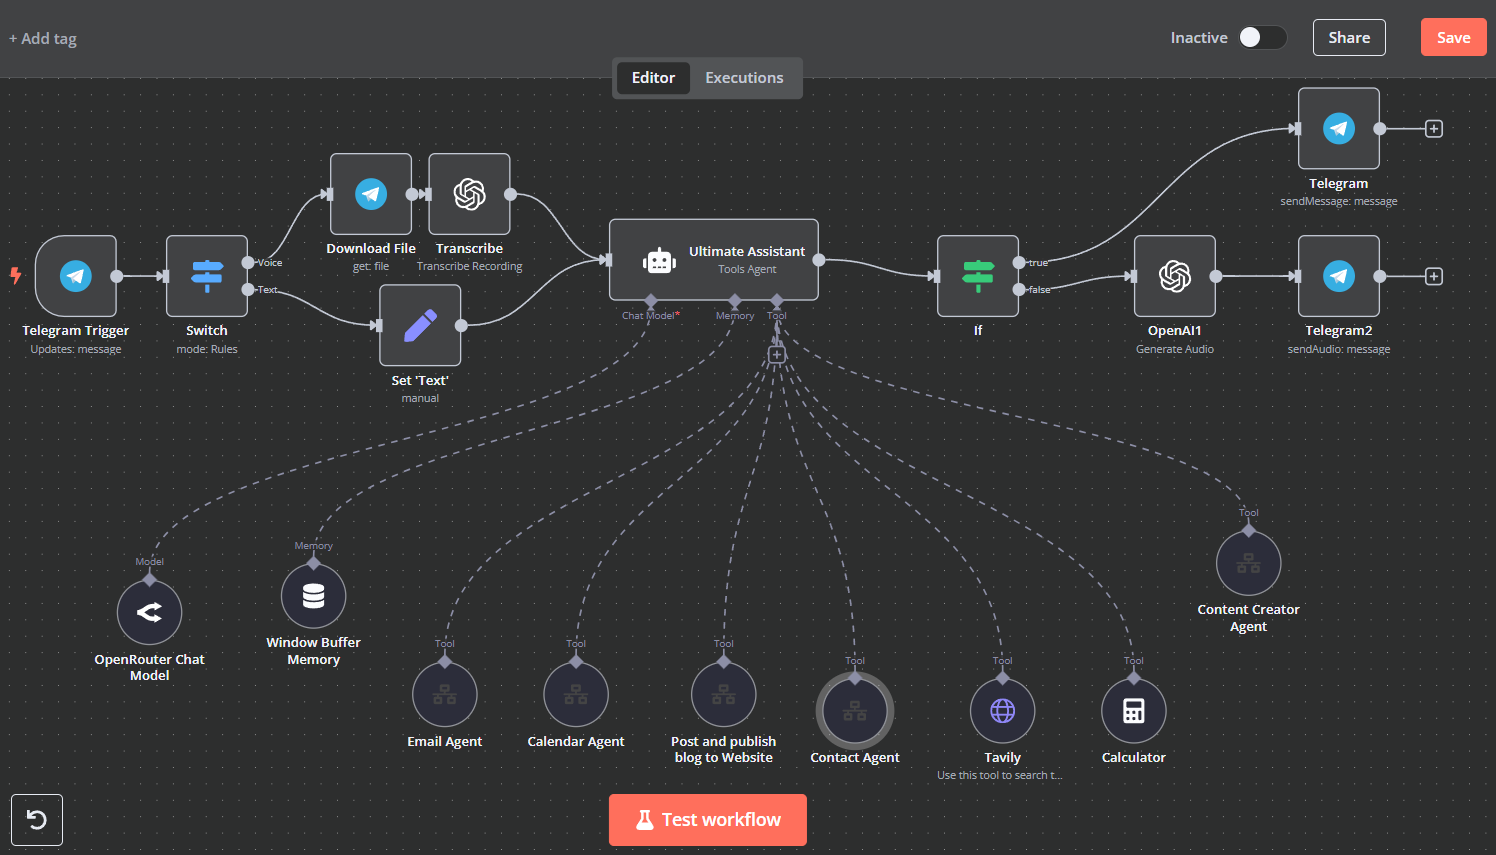
\includegraphics[width=1\textwidth]{images/4chatbot01.png}
    \caption{Workflow trợ lý ảo Telegram}
    \end{figure}


\subsection{Phân tích chi tiết công dụng và ưu điểm}

\subsubsection{Công dụng chính}
\begin{enumerate}
    \item \textbf{Trợ lý đa chức năng tự động}: Hệ thống hoạt động như một trợ lý cá nhân/văn phòng tự động xử lý nhiều loại tác vụ khác nhau.
    
    \item \textbf{Tích hợp đa nền tảng}: Kết nối Telegram làm giao diện người dùng với các dịch vụ Gmail, Google Calendar, Airtable và công cụ tìm kiếm.
    
    \item \textbf{Xử lý ngôn ngữ tự nhiên}: Người dùng có thể giao tiếp bằng văn bản hoặc giọng nói tự nhiên, không cần câu lệnh cụ thể.
    
    \item \textbf{Tự động hóa công việc hàng ngày}:
    \begin{itemize}
        \item Quản lý email: gửi, lấy, dán nhãn, tạo bản nháp
        \item Quản lý lịch: tạo, xóa, cập nhật sự kiện và cuộc họp
        \item Quản lý danh bạ: lưu trữ và truy xuất thông tin liên hệ
        \item Tạo nội dung: viết và xuất bản bài blog dựa trên nghiên cứu
    \end{itemize}
\end{enumerate}

\subsubsection{Ưu điểm nổi bật}
\begin{enumerate}
    \item \textbf{Kiến trúc module hóa}: Mỗi chức năng được phân tách thành agent riêng biệt, dễ bảo trì và mở rộng.
    
    \item \textbf{Tự động định tuyến tác vụ}: Hệ thống tự nhận diện yêu cầu và chuyển đến agent phù hợp.
    
    \item \textbf{Sử dụng LLM tiên tiến}: OpenRouter và OpenAI đảm bảo khả năng hiểu và xử lý ngôn ngữ tự nhiên chất lượng cao.
    
    \item \textbf{Xử lý lỗi thông minh}: Các agent đều có xử lý lỗi (error handling) để đảm bảo trải nghiệm người dùng mượt mà.
    
    \item \textbf{Cá nhân hóa cao}: Kết nối với tài khoản cá nhân của người dùng (email, lịch, danh bạ).
    
    \item \textbf{Đa dạng đầu vào}: Xử lý cả tin nhắn văn bản và ghi âm, tăng tính linh hoạt.
    
    \item \textbf{Tương tác hai chiều}: Cung cấp phản hồi kịp thời qua tin nhắn hoặc file âm thanh.
\end{enumerate}

\subsection{Hướng dẫn thiết lập credentials}

\subsubsection{Tổng quan về credentials cần thiết}
Để thiết lập toàn bộ hệ thống chatbot Ultimate Assistant, bạn cần cấu hình các xác thực (credentials) cho các dịch vụ sau:

\begin{itemize}
    \item Telegram Bot API
    \item OpenAI/OpenRouter API
    \item Google (Gmail và Calendar)
    \item Airtable
    \item Tavily Search API
\end{itemize}

Dưới đây là hướng dẫn chi tiết cách thiết lập từng loại credential:

\subsubsection{\underline{Telegram Bot API}}
\textbf{Mục đích}: Cho phép chatbot tương tác với người dùng qua Telegram.

\textbf{Cách thiết lập}:
\begin{enumerate}
    \item Mở Telegram và tìm kiếm \texttt{\href{https://telegram.me/BotFather}{@BotFather}}
    \item Gửi lệnh \texttt{/newbot} và làm theo hướng dẫn để tạo bot mới
    \item Đặt tên cho bot và username (phải kết thúc bằng ``bot'')
    \item BotFather sẽ cung cấp token API (dạng \texttt{123456789:ABCdefGhIJKlmNoPQRsTUVwxyZ})
    \item Trong n8n:
    \begin{itemize}
        \item Vào ``Credentials'' > ``New'' > ``Telegram API''
        \item Nhập Bot Token API đã nhận được
        \item Lưu credential với tên (ví dụ: ``Telegram account Hai'')
    \end{itemize}
\end{enumerate}

\subsubsection{\underline{OpenAI/OpenRouter API}}
\textbf{Mục đích}: Cung cấp mô hình ngôn ngữ (LLM) để chatbot hiểu và tạo phản hồi.

\paragraph{OpenAI API:}
\begin{enumerate}
    \item Đăng ký tài khoản tại \href{https://platform.openai.com/}{OpenAI}
    \item Truy cập ``API Keys'' và tạo key mới
    \item Trong n8n:
    \begin{itemize}
        \item Vào ``Credentials'' > ``New'' > ``OpenAI API''
        \item Nhập API Key
        \item Lưu credential với tên (ví dụ: ``OpenAi account'')
    \end{itemize}
\end{enumerate}

\paragraph{OpenRouter API} (thay thế cho OpenAI): thay đổi nhiều model LLM 
\begin{enumerate}
    \item Đăng ký tại \href{https://openrouter.ai/}{OpenRouter}
    \item Tạo API key mới
    \item Trong n8n:
    \begin{itemize}
        \item Vào ``Credentials'' > ``New'' > ``OpenRouter API''
        \item Nhập API Key
        \item Lưu credential với tên (ví dụ: ``OpenRouter account'')
    \end{itemize}
\end{enumerate}

\subsubsection{\underline{Google (Gmail và Calendar)}}
\textbf{Mục đích}: Cho phép chatbot truy cập và quản lý email và lịch.

\textbf{Thiết lập Google OAuth2}:
\begin{enumerate}
    \item Truy cập \href{https://console.cloud.google.com/}{Google Cloud Console}
    \item Tạo project mới hoặc chọn project sẵn có
    \item Đi tới ``APIs \& Services'' > ``Library''
    \item Kích hoạt các API: Gmail API và Google Calendar API
    \item Đi tới ``OAuth consent screen'':
    \begin{itemize}
        \item Chọn loại người dùng (External/Internal)
        \item Nhập thông tin ứng dụng (tên, email liên hệ)
        \item Thêm scopes cần thiết: Gmail (send, read, modify) và Calendar (read, write)
    \end{itemize}
    \item Tạo OAuth2 credentials:
    \begin{itemize}
        \item Đi tới ``Credentials'' > ``Create Credentials'' > ``OAuth client ID''
        \item Chọn Application Type: ``Web application''
        \item Thêm Redirect URI: URL từ n8n (thường có dạng \url{https://your-n8n-instance.com/rest/oauth2-credential/callback})
    \end{itemize}
    \item Trong n8n:
    \begin{itemize}
        \item Vào ``Credentials'' > ``New'' > ``OAuth2 API'' (cho Gmail hoặc Google Calendar)
        \item Nhập Client ID và Client Secret từ Google Cloud
        \item Nhập các scopes cần thiết
        \item Nhấn ``Connect'' và xác thực với tài khoản Google của bạn
        \item Lưu credentials với tên phù hợp (ví dụ: ``Gmail account'', ``Google Calendar account'')
    \end{itemize}
\end{enumerate}

\subsubsection{\underline{Airtable}}
\textbf{Mục đích}: Lưu trữ và quản lý thông tin liên hệ.

\textbf{Thiết lập Airtable API}:
\begin{enumerate}
    \item Đăng nhập vào \href{https://airtable.com/}{Airtable}
    \item Tạo một base mới với bảng ``Contacts'' chứa các trường: name, email, phoneNumber
    \item Truy cập ``Account'' > ``Developer Hub'' > ``Personal Access Tokens''
    \item Tạo token mới với quyền truy cập phù hợp
    \item Trong n8n:
    \begin{itemize}
        \item Vào ``Credentials'' > ``New'' > ``Airtable API''
        \item Nhập API Key
        \item Lưu credential với tên phù hợp
    \end{itemize}
    \item Lấy Base ID:
    \begin{itemize}
        \item Mở Airtable base của bạn
        \item Xem URL: \texttt{https://airtable.com/[BASE\_ID]/[TABLE\_ID]/[VIEW\_ID]}
        \item Lưu lại BASE\_ID để sử dụng trong workflow
    \end{itemize}
\end{enumerate}

\subsubsection{\underline{Tavily Search API}}
\textbf{Mục đích}: Cho phép chatbot tìm kiếm thông tin trên web.

\textbf{Thiết lập Tavily API}:
\begin{enumerate}
    \item Đăng ký tài khoản tại \href{https://tavily.com/}{Tavily}
    \item Nhận API key từ dashboard
    \item Trong workflow n8n:
    \begin{itemize}
        \item Tại nút HTTP Request Tool, nhập trực tiếp API key vào JSON body:
    \end{itemize}
\end{enumerate}

\begin{lstlisting}[language=json, basicstyle=\small\ttfamily]
{
  "api_key": "tvly-YOUR_API_KEY",
  "query": "{searchTerm}",
  "search_depth": "basic",
  "include_answer": true,
  "topic": "news",
  "include_raw_content": true,
  "max_results": 3
}
\end{lstlisting}

\subsubsection{\underline{Kiểm tra và xác minh credentials}}
Sau khi cài đặt tất cả credentials:
\begin{itemize}
    \item Kiểm tra từng workflow để đảm bảo nó được liên kết với credential đúng
    \item Thực hiện kiểm tra kết nối cho mỗi credential trong n8n
    \item Chạy thử từng workflow thành phần trước khi tích hợp vào hệ thống chính
\end{itemize}

\subsubsection{\underline{Lưu ý bảo mật}}
\begin{itemize}
    \item \textbf{Không chia sẻ API keys}: Bảo vệ tất cả credentials và không chia sẻ trong code công khai
    \item \textbf{Giới hạn quyền truy cập}: Chỉ cấp quyền cần thiết cho mỗi API
    \item \textbf{Theo dõi sử dụng}: Giám sát việc sử dụng API để tránh vượt quá giới hạn
    \item \textbf{Luân chuyển keys}: Cập nhật keys định kỳ theo các thực hành bảo mật tốt nhất
    \item \textbf{Mã hóa credentials}: n8n mã hóa credentials, nhưng hãy đảm bảo máy chủ n8n được bảo mật
\end{itemize}

Với tất cả các credentials được thiết lập đúng cách, Ultimate Assistant Chatbot của bạn sẽ có thể tương tác với Telegram và điều phối tất cả các dịch vụ bên ngoài một cách liền mạch.

\clearpage
%----------------------------------------------------------------------
\section{\textbf{Dự án 4: Tạo short video hoạt hình bằng AI và đăng lên youtube }}

\href{https://drive.google.com/file/d/1hBEgM7DZBiMOocM_pxGyne7T97oAKK_B/view?usp=sharing}{\textbf{\underline {Link tải workflow}}}

\begin{figure}[h]
    \centering
    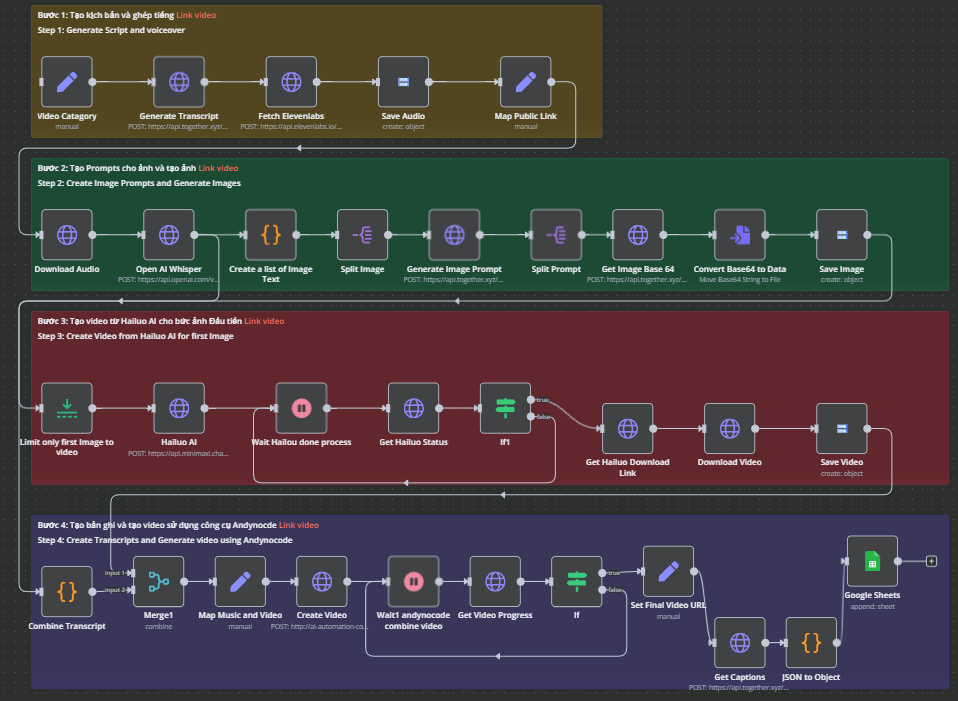
\includegraphics[width=1\textwidth]{images/Da1-01.png}
    \caption{Workflow kết quả dự án 1}
    
\end{figure}

Trong ví dụ này chúng ta sẽ làm một workflow để tạo short video animated. \\

\underline{Ứng dụng:}\\
\begin{itemize}[label=-]
    \item Nhà tiếp thị muốn tạo video quảng cáo tự động, nhanh chóng
    \item Người sáng tạo nội dung muốn tối ưu hóa quy trình sản xuất video
    \item Doanh nghiệp tìm kiếm phương pháp hiệu quả để giới thiệu sản phẩm 
\end{itemize}


\underline{Ý tưởng thiết kế:}\\
\begin{figure}[h]
    \centering
    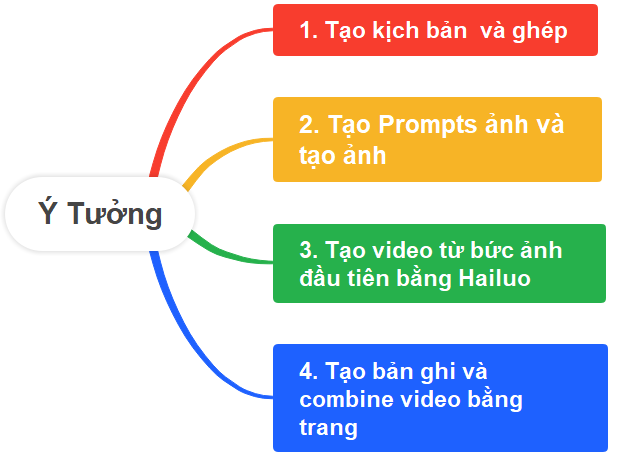
\includegraphics[width=0.7\textwidth]{images/Da1-02.png}
    \caption{Ý tưởng thiết kế}
    
\end{figure}


\underline{Các công cụ sử dụng trong workflow:}\\
\begin{itemize}[label=-]
    \item \textbf{Tạo giọng nói AI với ElevenLabs}: Sử dụng \textbf{\emph{ElevenLabs}}, quy trình này chuyển đổi văn bản thành giọng nói tự nhiên, giúp video trở nên sống động và chuyên nghiệp hơn. ElevenLabs AI là một nền tảng AI Text-to-Speech (TTS) giúp chuyển đổi văn bản thành giọng nói tự nhiên, chân thực với nhiều giọng đọc và ngôn ngữ khác nhau. Nó thường được dùng để tạo giọng nói nhân tạo phục vụ video, podcast, ứng dụng AI, chatbot và nhiều mục đích khác. ElevenLabs AI giúp tự động hóa quy trình tạo giọng nói từ văn bản. Dùng trong một số ứng dụng thực tế như: Chuyển đổi văn bản thành giọng nói (TTS) tự động, Tạo chatbot có giọng nói nhân tạo, Đọc báo, thông tin hoặc tin tức tự động, Tổng đài AI tự động (Voice AI Callbot)
    \item \textbf{Chuyển đổi ảnh thành video với Hailuo AI}: Với  \textbf{\emph{Hailuo AI}} hình ảnh tĩnh được chuyển đổi thành video động, giúp tạo nội dung trực quan hấp dẫn mà không cần chỉnh sửa thủ công. Các ứng dụng mà Hailou AI có thể làm.\\

    + Chuyển đổi văn bản thành video: Hailuo AI giúp biến những đoạn văn bản thành video sống động, tối ưu hóa quy trình sáng tạo nội dung và tiết kiệm thời gian cho người dùng.\\
    + Chuyển đổi hình ảnh thành video: Người dùng có thể tải lên hình ảnh tĩnh và nhập mô tả; Hailuo AI sẽ tạo ra video dựa trên nội dung đó, mang lại trải nghiệm trực quan và sinh động.\\
    + Chuyển đổi văn bản thành giọng nói (Text-to-Speech): Hailuo AI cung cấp tính năng chuyển đổi văn bản thành giọng nói với nhiều ngôn ngữ và giọng đọc tự nhiên, hỗ trợ đa dạng nhu cầu của người dùng. 
    \item \textbf{Cải thiện nội dung với Together AI}: Để đảm bảo chất lượng nội dung cao, \textbf{\emph{Together AI}} tối ưu hóa và điều chỉnh lời nhắc, giúp tạo ra các kịch bản hấp dẫn và phù hợp hơn. Nó giống một bên trung gian để chung ta truy cập vào các mô hình AI.
    \item \textbf{Xử lý thông minh với OpenAI}: Các tác vụ suy luận, như tạo nội dung văn bản và tối ưu hóa nội dung, được thực hiện bởi \textbf{\emph{OpenAI}}, giúp quy trình sản xuất video diễn ra trơn tru và hiệu quả. 
    \item \textbf{Tích hợp với Google Sheets}: Sau khi tạo video, \textbf{\emph{URL tải xuống}} sẽ được tự động tải lên \textbf{\emph{Google Sheets}}, giúp người dùng dễ dàng truy cập và quản lý nội dung. 
     \item \textbf{Lưu trữ thông tin bằng Google Cloud Storage}: Node \textbf{\emph{Google Cloud Storage}} trong n8n giúp bạn làm việc với dịch vụ lưu trữ đám mây Google Cloud Storage (GCS). Nó cho phép bạn tải lên, tải xuống, xóa và quản lý tệp trên Google Cloud Storage Buckets trong quy trình tự động hóa của mình. 
     \item \textbf{Tối ưu hóa với node code}: Node Code trong n8n cho phép bạn viết JavaScript để xử lý dữ liệu tùy chỉnh trong quy trình tự động hóa. Nó giúp mở rộng khả năng của n8n khi các node có sẵn không đáp ứng đủ nhu cầu.   
\end{itemize}

\underline{\textbf{ Các bước triển khai:}}

\subsection{Tạo node "Edit Fields}

\begin{itemize}
    \item[-] Tạo các trường dữ liệu (data fields): Node Edit File cho phép tạo ra các trường dữ liệu mới và gán giá trị cho chúng.
    \item[-] Mapping (ánh xạ) dữ liệu: Node Edit File được sử dụng để ánh xạ dữ liệu từ các nguồn khác nhau và kết hợp chúng lại với nhau. Ví dụ: Ánh xạ URL của audio đã tạo, Kết hợp URL của video và nhạc nền. Thiết lập các tham số (parameters): Node Edit File được sử dụng để thiết lập các tham số cần thiết cho các bước tiếp theo trong quy trình.
    \item[-] Chỉnh sửa thông tin: Node Edit File có thể chỉnh sửa các thông tin khác nhau.
\end{itemize}  
    \begin{figure}[H]
 
    \centering
    \begin{minipage}{0.5\textwidth}
        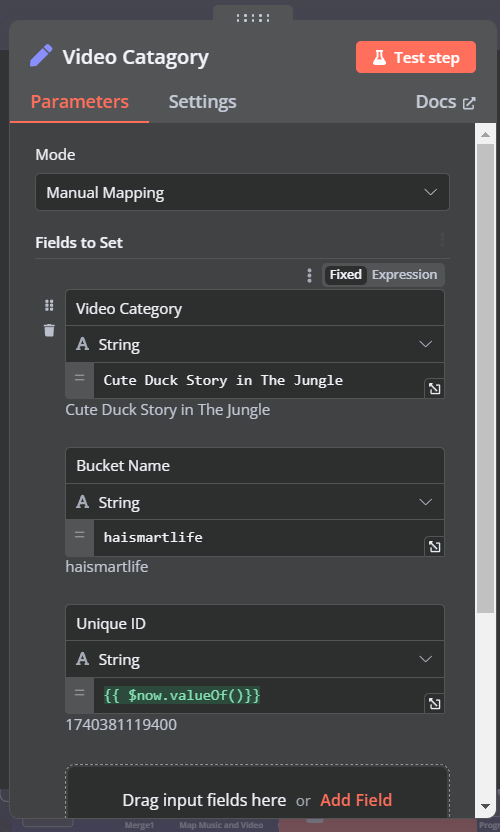
\includegraphics[width=\linewidth]{images/Da1-03.png}
    \end{minipage}
    %\hfill
    \hspace{5pt}
    \begin{minipage}{0.4\textwidth}
    
        \underline{Các thông số cần cài đặt:}\\
        \begin{itemize}[label=\textbullet]
            \item Đổi tên node thành \emph{"Video Catagory"}
            \item Mục Mode: Chọn \emph{"Manual Mapping"}
            \item Mục Fields to Set: Chọn "Add Field" và tạo 3 trường như hình bên cạnh, trong đó:\\
            
            \textbf{\emph{"Video Category"}} là trường  nội dung video bạn muốn tạo, thay thế thành loại video hoặc nội dung bạn muốn.\\
            \textbf{\emph{"Bucket Name"}} là tên của bucket mà bạn sẽ tạo trong google cloud để lưu các hình ảnh, âm thanh AI tạo ra.\\
            \textbf{\emph{"Unique ID"}} bằng giá trị "\verb|{{$now.valueOf()}}|" là một tham số quan trọng để đảm bảo tính duy nhất và chính xác của các tệp trong quy trình tạo video tự động, đặc biệt là để ngăn chặn các vấn đề liên quan đến caching.\\

            
        \end{itemize}
    \end{minipage}
\end{figure}
     
    % \item 
    % \item 
    % \item 
    % \item 


\subsection{Elevenlabs - AI về âm thanh, chuyển đổi text và voice.}
\begin{itemize}[label=]
    \item \textbf{Bước 1: Tạo API key Elevenlabs} 
    
    Truy cập vào link \url{https://elevenlabs.io/app/settings/api-keys} \\ 
    
    Tìm đến API key và nhấn tạo ta sẽ được dãy ký tự, sau đó hãy copy nó.\\
    
    Lưu ý: API này dùng free sẽ hay bị lỗi nên nếu xây dựng được một workflow hữu ích thì nên mua để tránh gặp các lỗi không mong muốn.\\
    
    \begin{figure}[H]
    \centering
    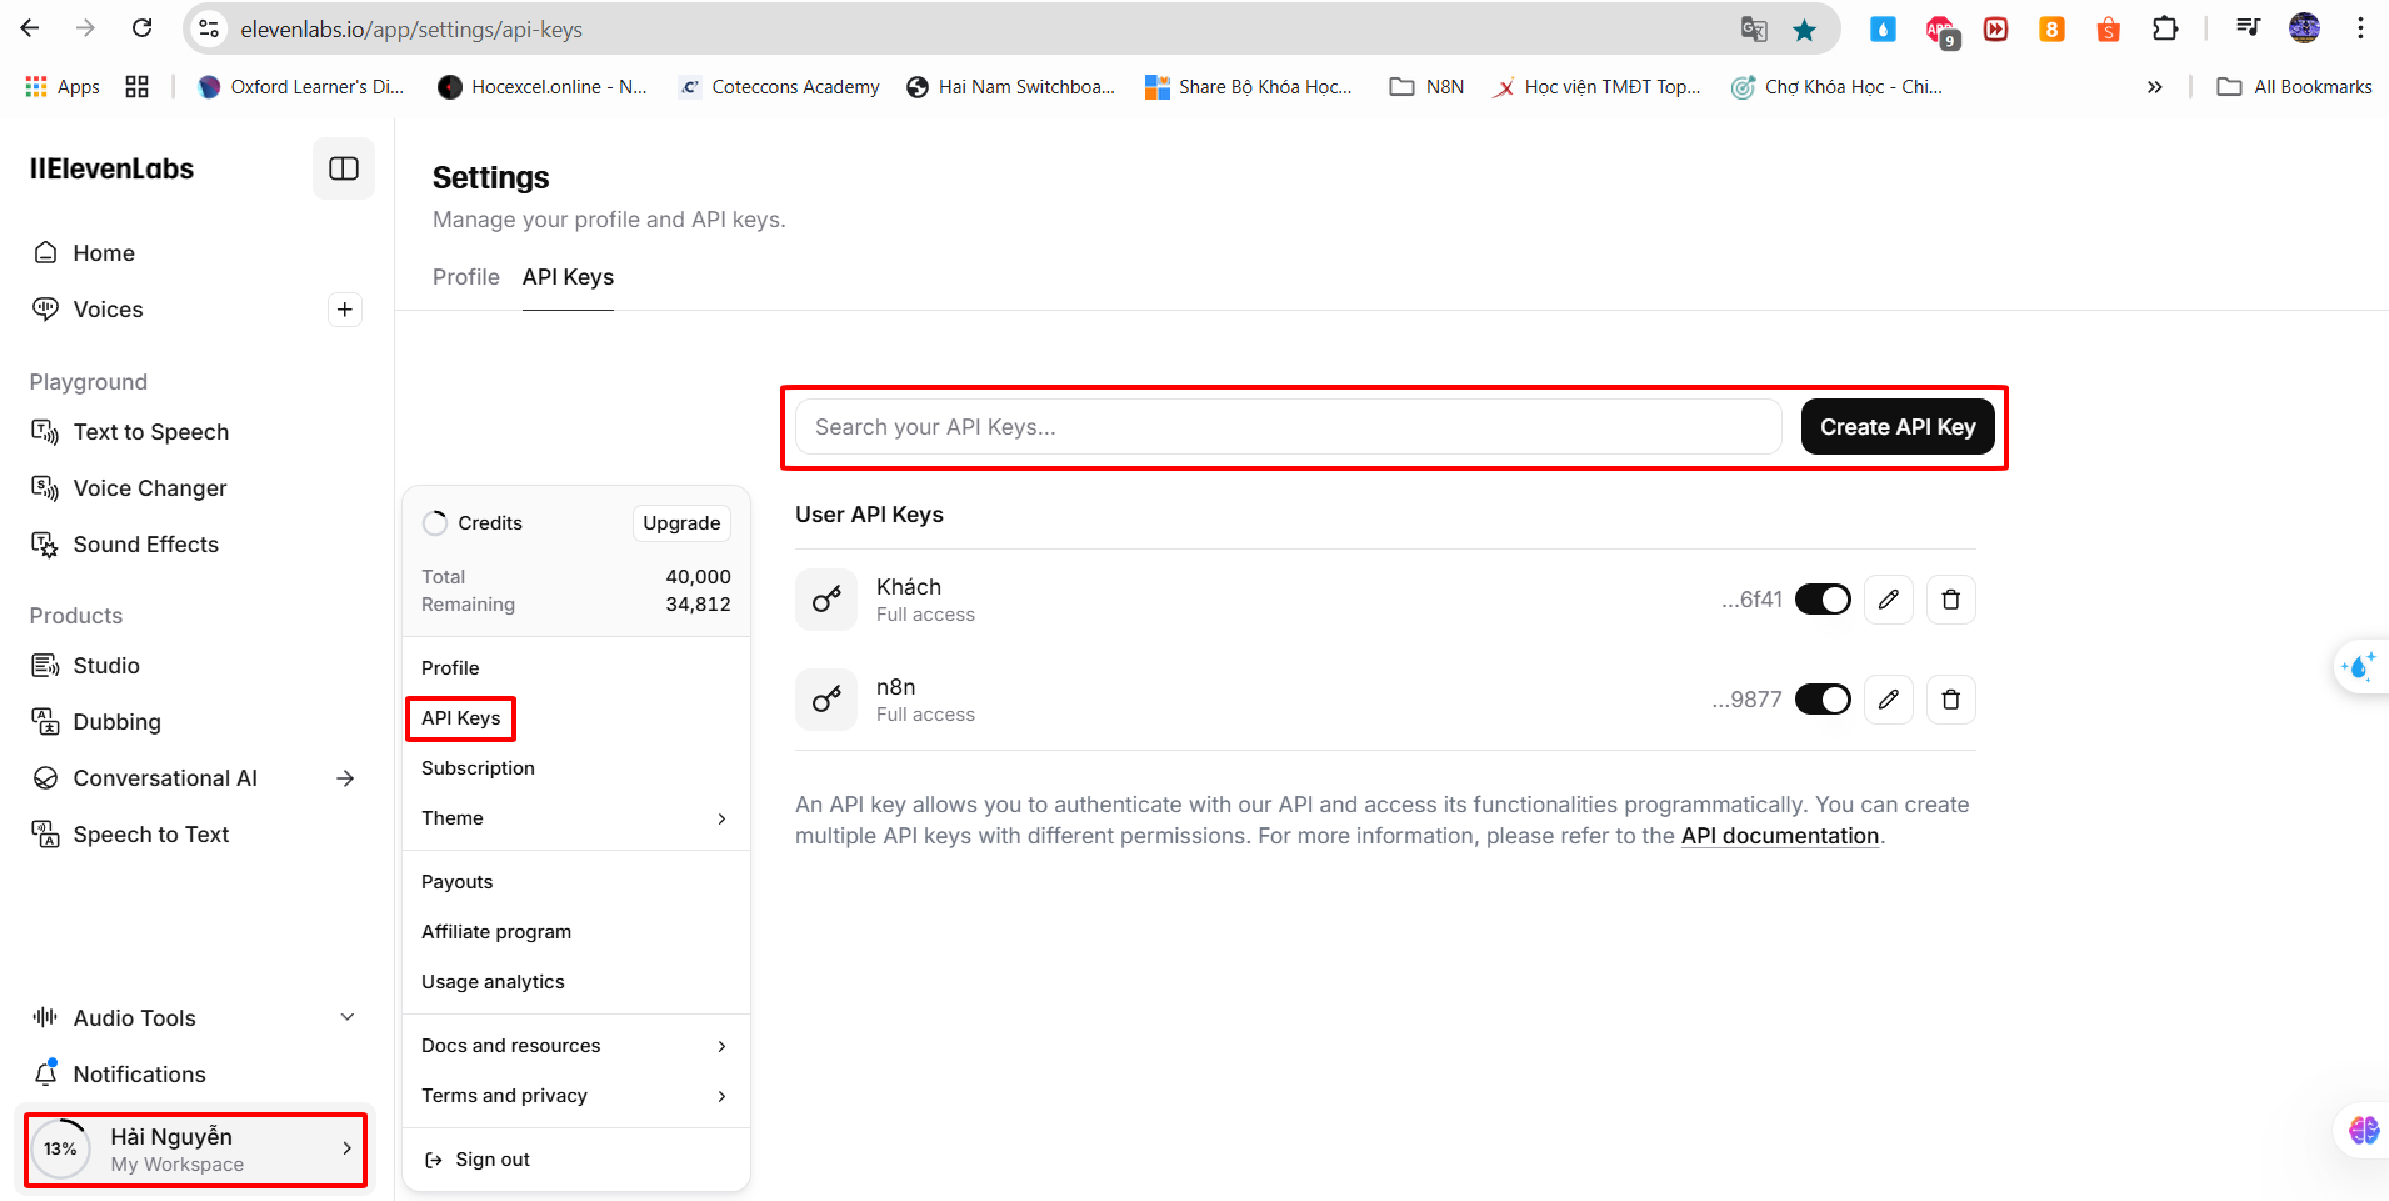
\includegraphics[width=1.0\textwidth]{images/Elevenlabs.pdf}
    \caption{Tạo API Elevenlabs}
    
    \end{figure}
 Tạo được API có dạng " sk\_7529a9c2502bb52789fa8cfcdafdc645c5edc038244e3136 " \\
 
    \begin{figure}[H]
    \centering
    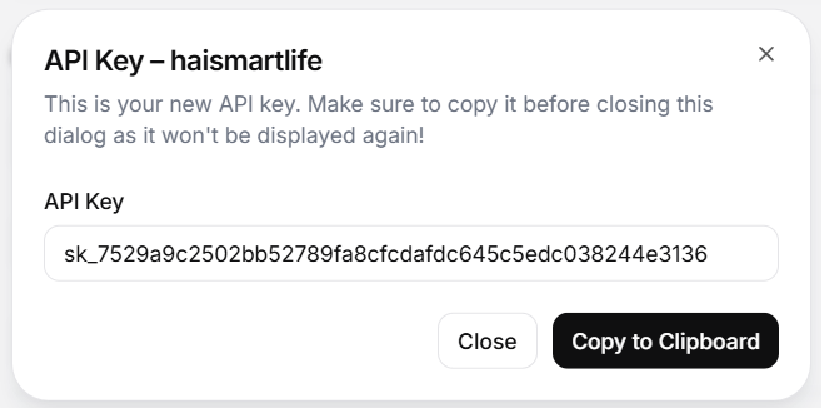
\includegraphics[width=0.6\textwidth]{images/Elevenlabs-1.pdf}
    \caption{Tạo API Elevenlabs}
    
    \end{figure}

    \item \textbf{Bước 2: Tạo node "HTTP truy cập Elevenlabs" trong n8n}\\
    
    \begin{figure}[h]
 
    \centering
    \begin{minipage}{0.45\textwidth}
        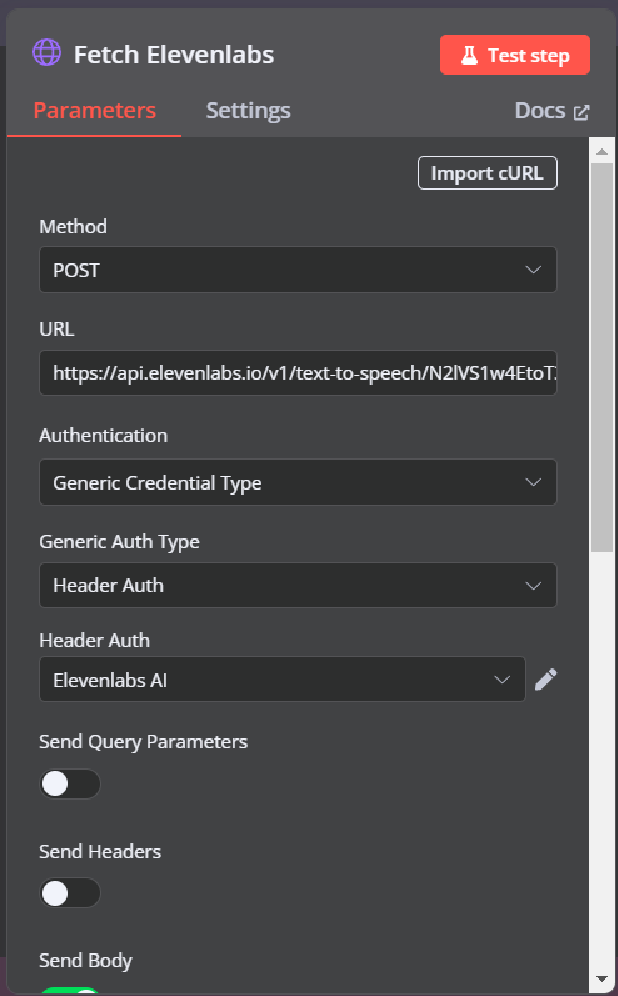
\includegraphics[width=\linewidth]{images/Elevenlabs-2.pdf}
    \end{minipage}
    %\hfill
    \hspace{5pt}
    \begin{minipage}{0.45\textwidth}
         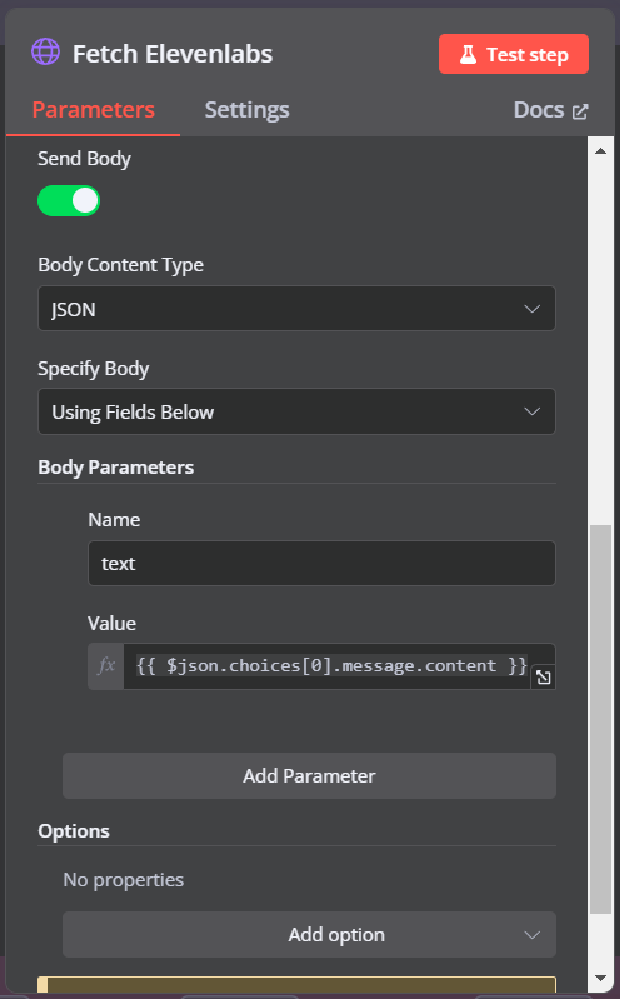
\includegraphics[width=\linewidth]{images/Elevenlabs-3.pdf}
    \end{minipage}
\end{figure}

Tại mục URL nhập: \\
"https://api.elevenlabs.io/v1/text-to-speech/N2lVS1w4EtoT3dr4eOWO"\\

Trong đó "N2lVS1w4EtoT3dr4eOWO" chính là ID của giọng nói mà các bạn muốn xuất hiện trong video

 \begin{figure}[H]
    \centering
    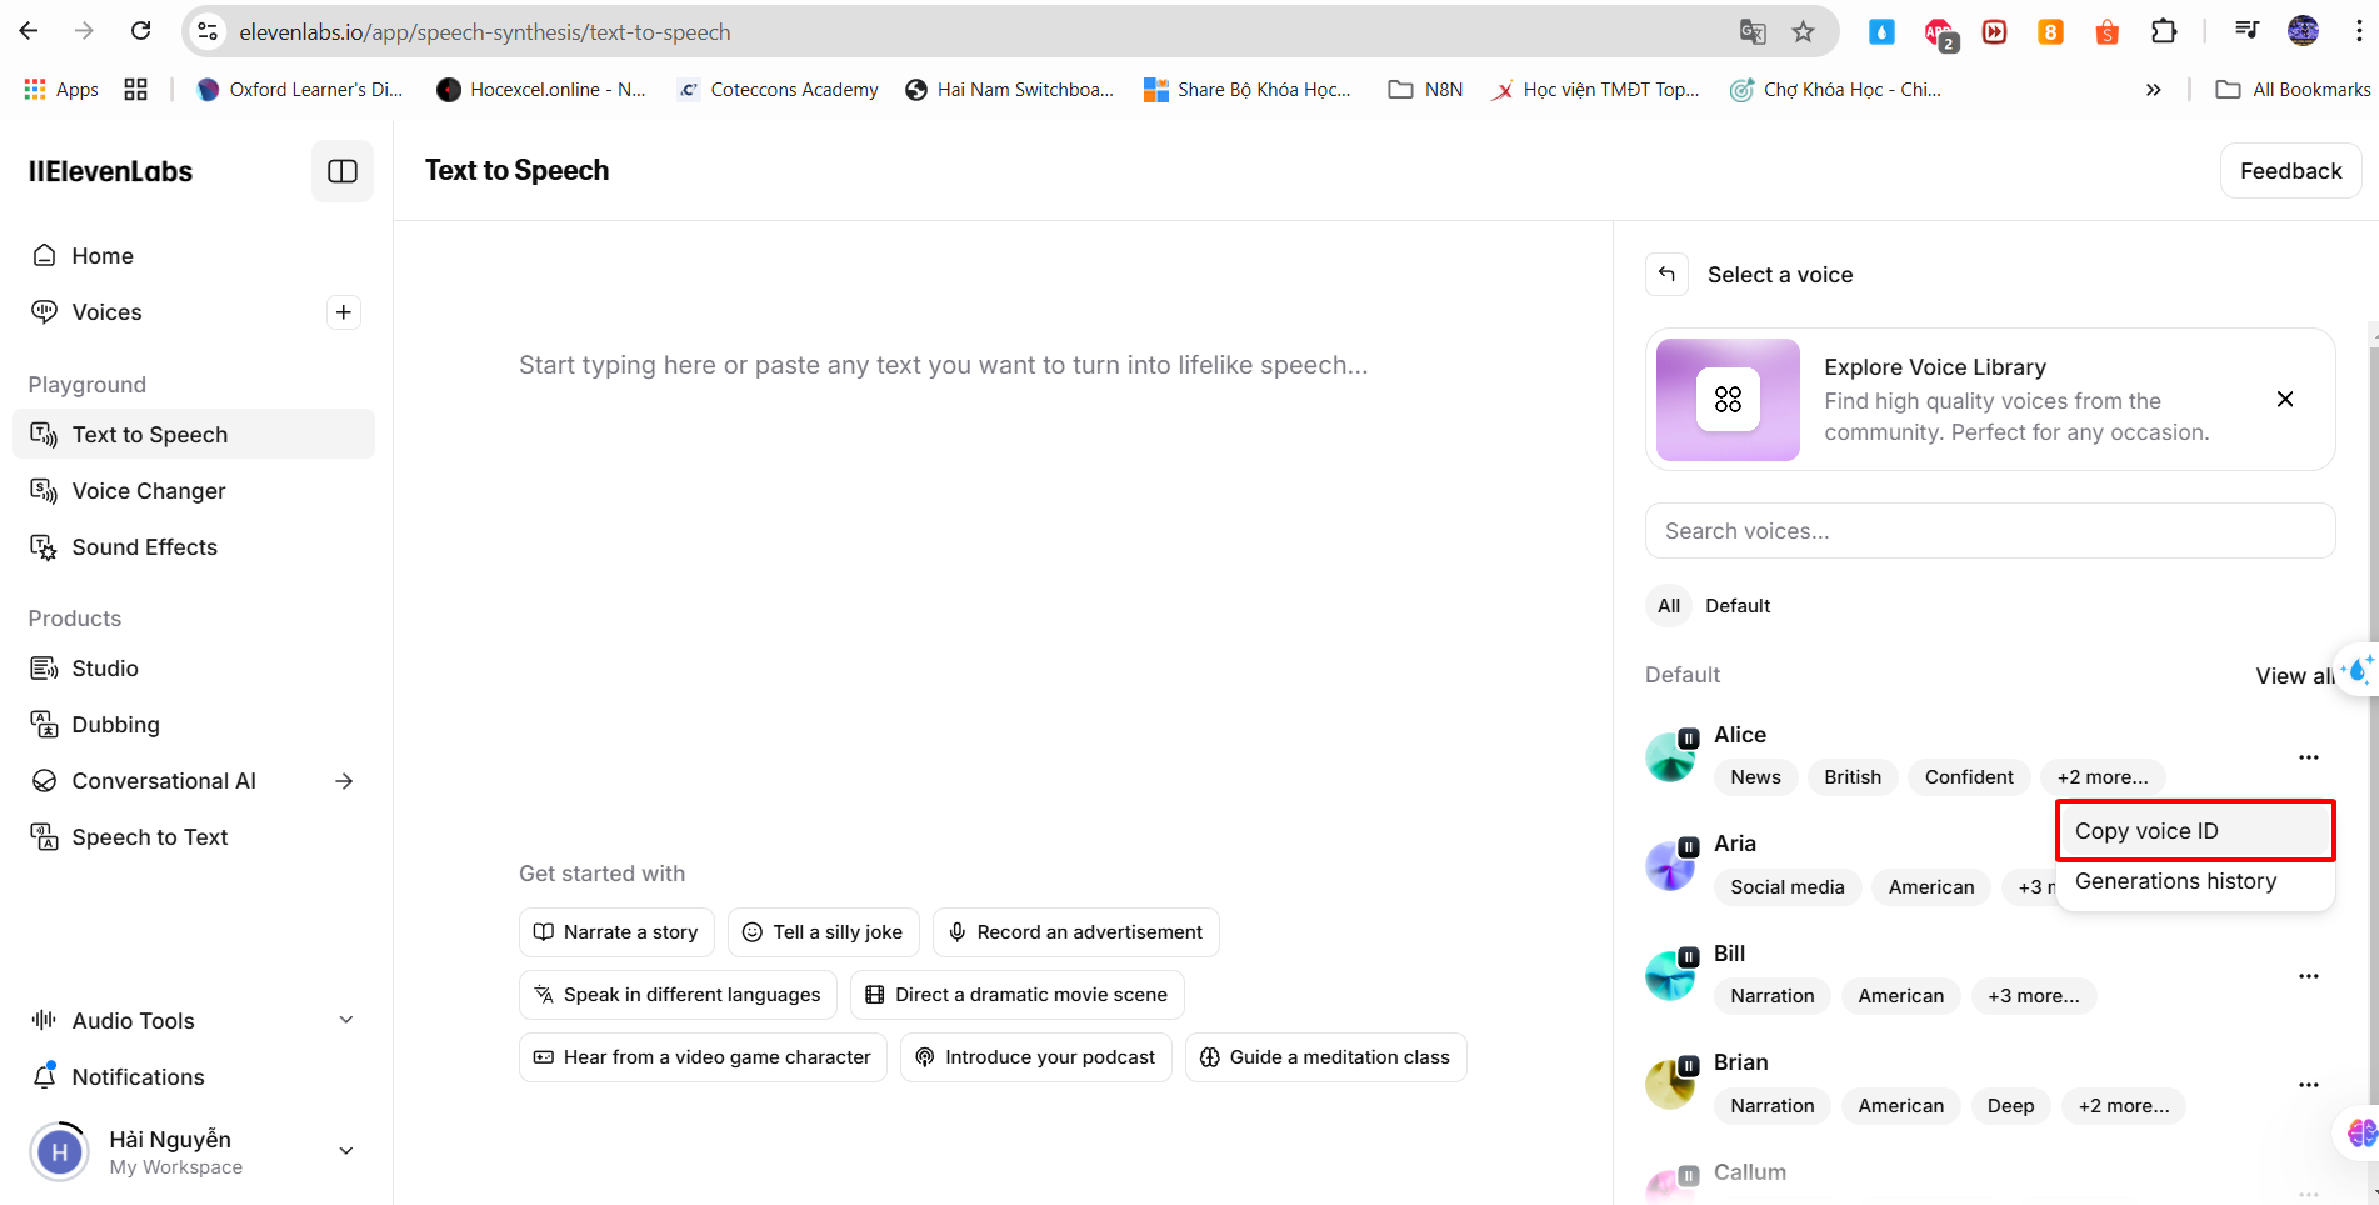
\includegraphics[width=1\textwidth]{images/Elevenlabs-4.pdf}
    \caption{Tạo API Elevenlabs}
    
    \end{figure}

 \begin{figure}[H]
    \centering
    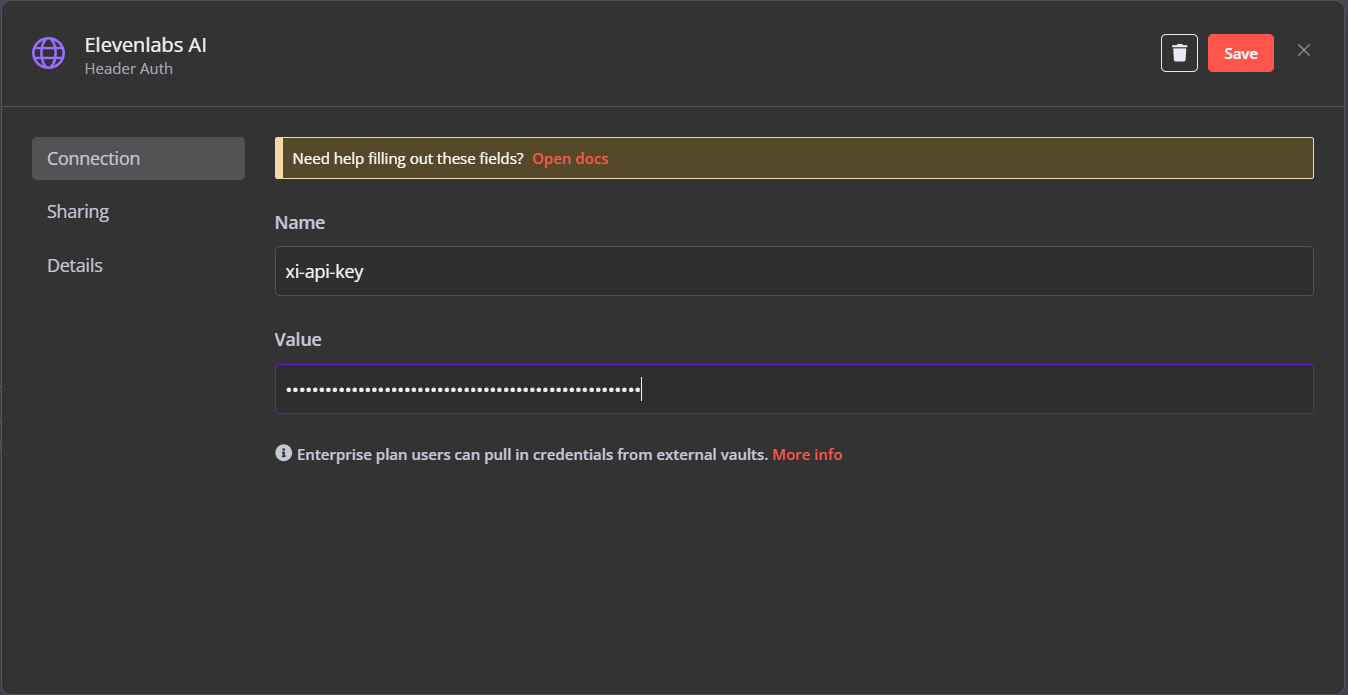
\includegraphics[width=1\textwidth]{images/Elevenlabs-5.png}
    \caption{Tạo API Elevenlabs}
    
    \end{figure}
    Set up credential cho Elevenlabs như hình bên dưới:\\
    Name: xi-api-key\\
    Value: " sk\_7529a9c2502bb52789fa8cfcdafdc645c5edc038244e3136 " (Paste API copy từ web Elevenlabs) \\

\end{itemize}

%--------------------------------------------------------------

\subsection{Together AI - nền tảng hỗ trợ các module AI tối ưu kết quả.}
\begin{itemize}[label=]
    \item \textbf{Bước 1: Tạo API key Together AI} 
    
    Truy cập vào link \url{https://api.together.ai/settings/api-keys} \\ 
    Tìm đến API keys và copy nó ta sẽ được dãy ký tự.\\
    Lưu ý: Thêm thông tin thẻ thanh toán và sử dụng như thường, và có thể thay node này bằng node khác có chức năng tương đương thể thử.\\
    
    \begin{figure}[H]
    \centering
    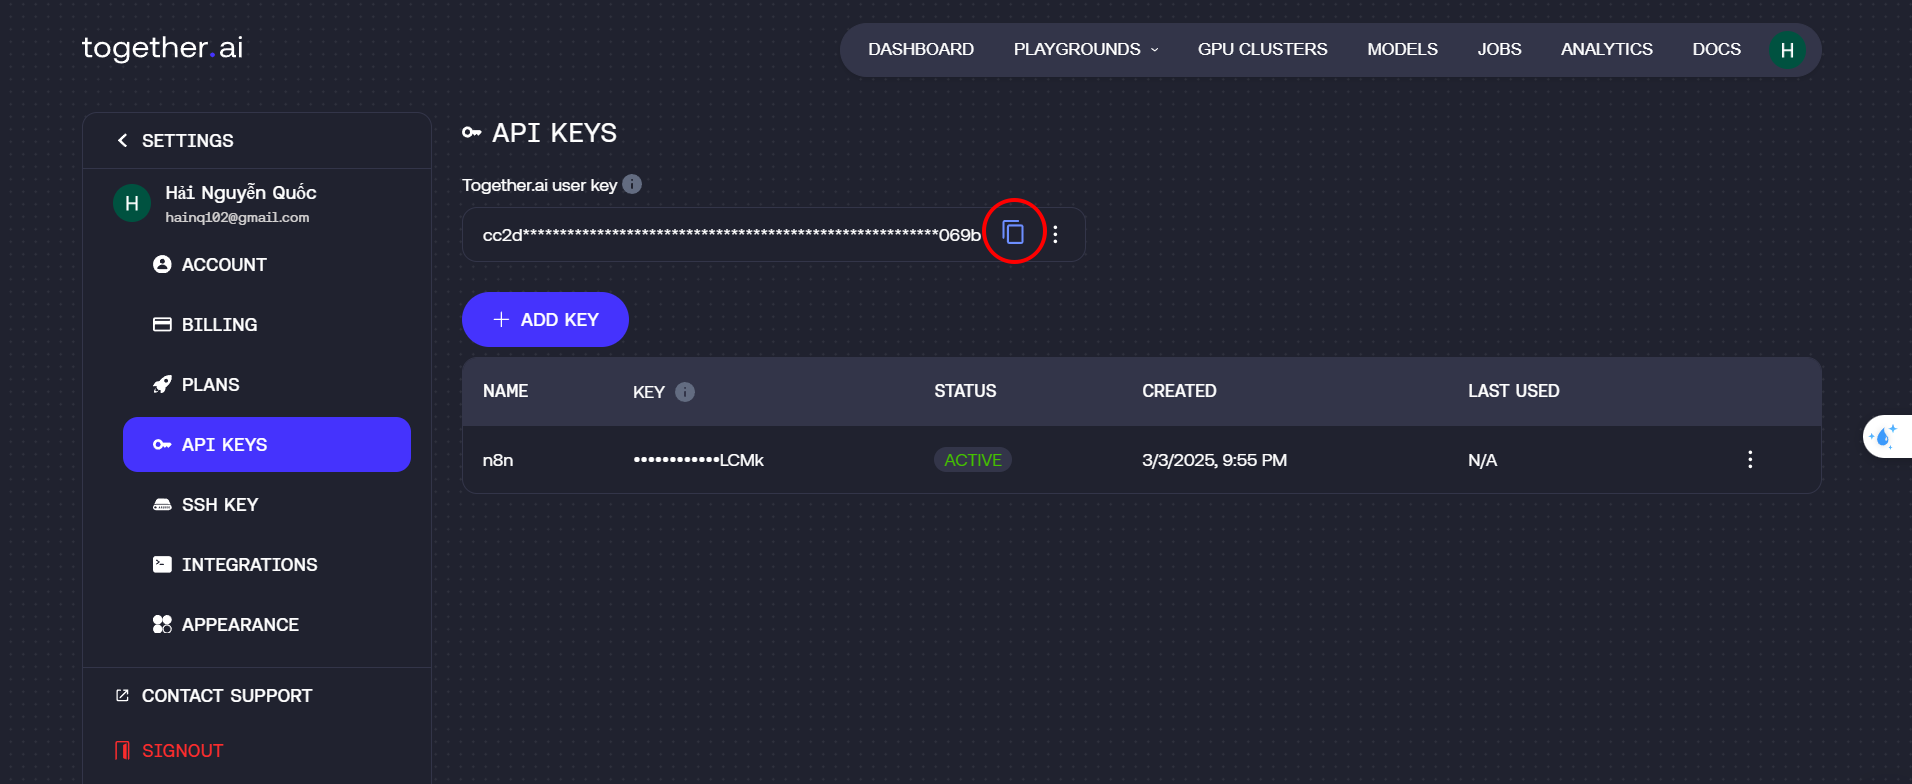
\includegraphics[width=0.95\textwidth]{images/TogetherAI.png}
    \caption{Tạo API Together AI}
    
    \end{figure}
    \item \textbf{Bước 2: Tạo node "HTTP truy cập Together AI" trong n8n}\\
    \begin{figure}[H]
    \centering
    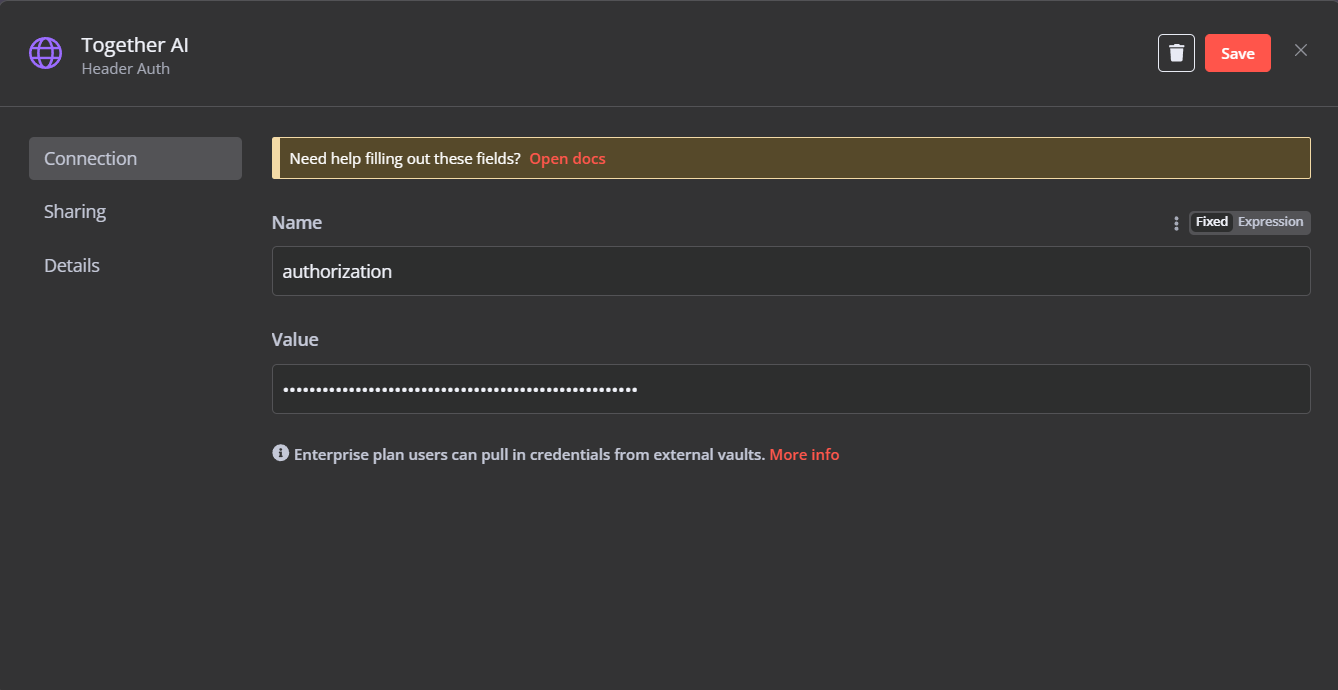
\includegraphics[width=0.95\textwidth]{images/TogetherAI-1.png}
    \caption{Tạo API Together AI}
    
    \end{figure}
    
 Tạo Node HTTP trong n8n, trong phần Header Auth chúng ta tạo credential như hình trên:\\
 Name: authorization\\
 Value: API vừa copy ở web Together AI\\
 
    \begin{figure}[H]
    \centering
    \begin{minipage}{0.45\textwidth}
        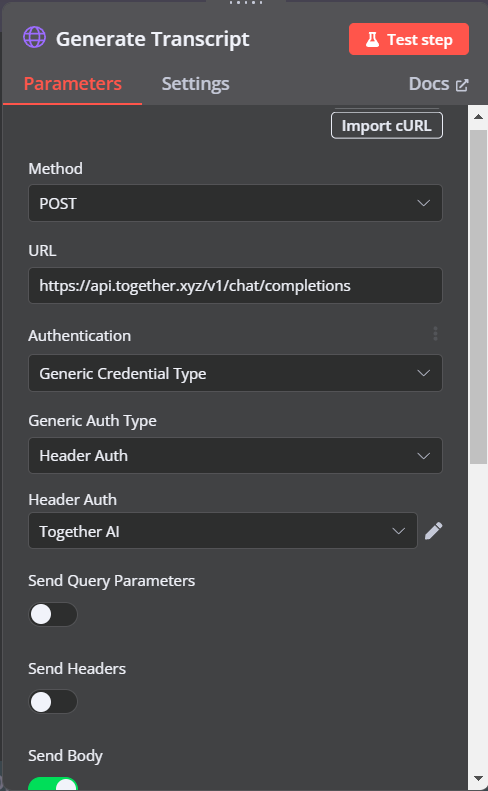
\includegraphics[width=\linewidth]{images/TogetherAI-2.png}
    \end{minipage}
    %\hfill
    \hspace{5pt}
    \begin{minipage}{0.45\textwidth}
         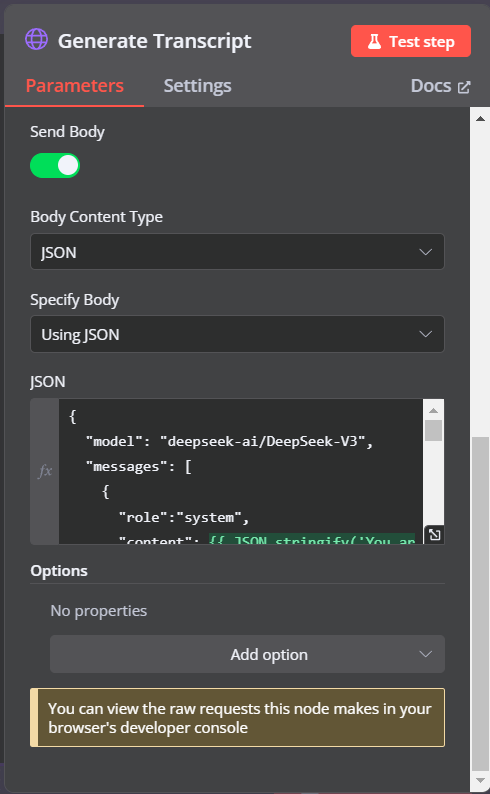
\includegraphics[width=\linewidth]{images/TogetherAI-3.png}
    \end{minipage}
\end{figure}

Tại mục URL nhập: \\
"https://api.together.xyz/v1/chat/completions"\\


\end{itemize}

%------------------------------------------------------
\subsection{Google cloud storage - Lưu trữ các video, Audio, Hình ảnh tạo ra}
\begin{itemize}[label=]
    \item \textbf{Bước 1: Set up tài khoản} 
    
    Truy cập vào link \url{https://console.cloud.google.com/} \\ 

    \begin{figure}[H]
    \centering
    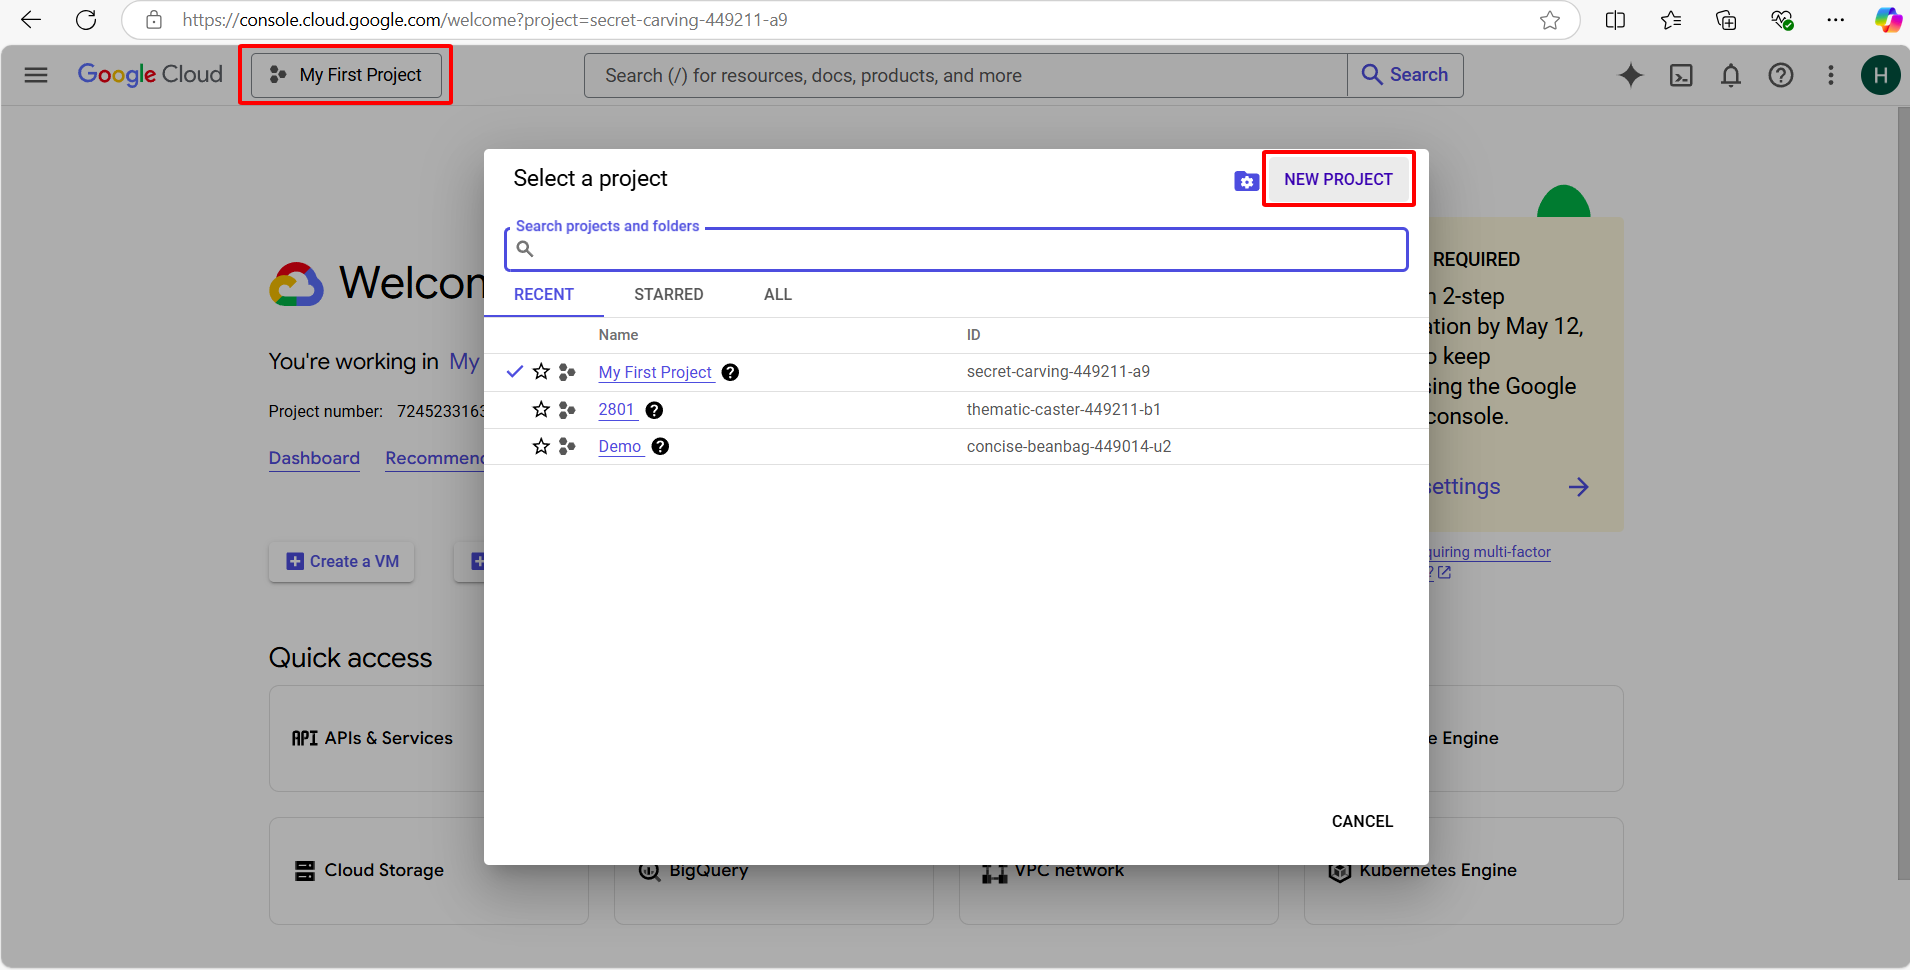
\includegraphics[width=0.95\textwidth]{images/GGcloud.png}
    
    \end{figure}
    \begin{figure}[H]
    \centering
    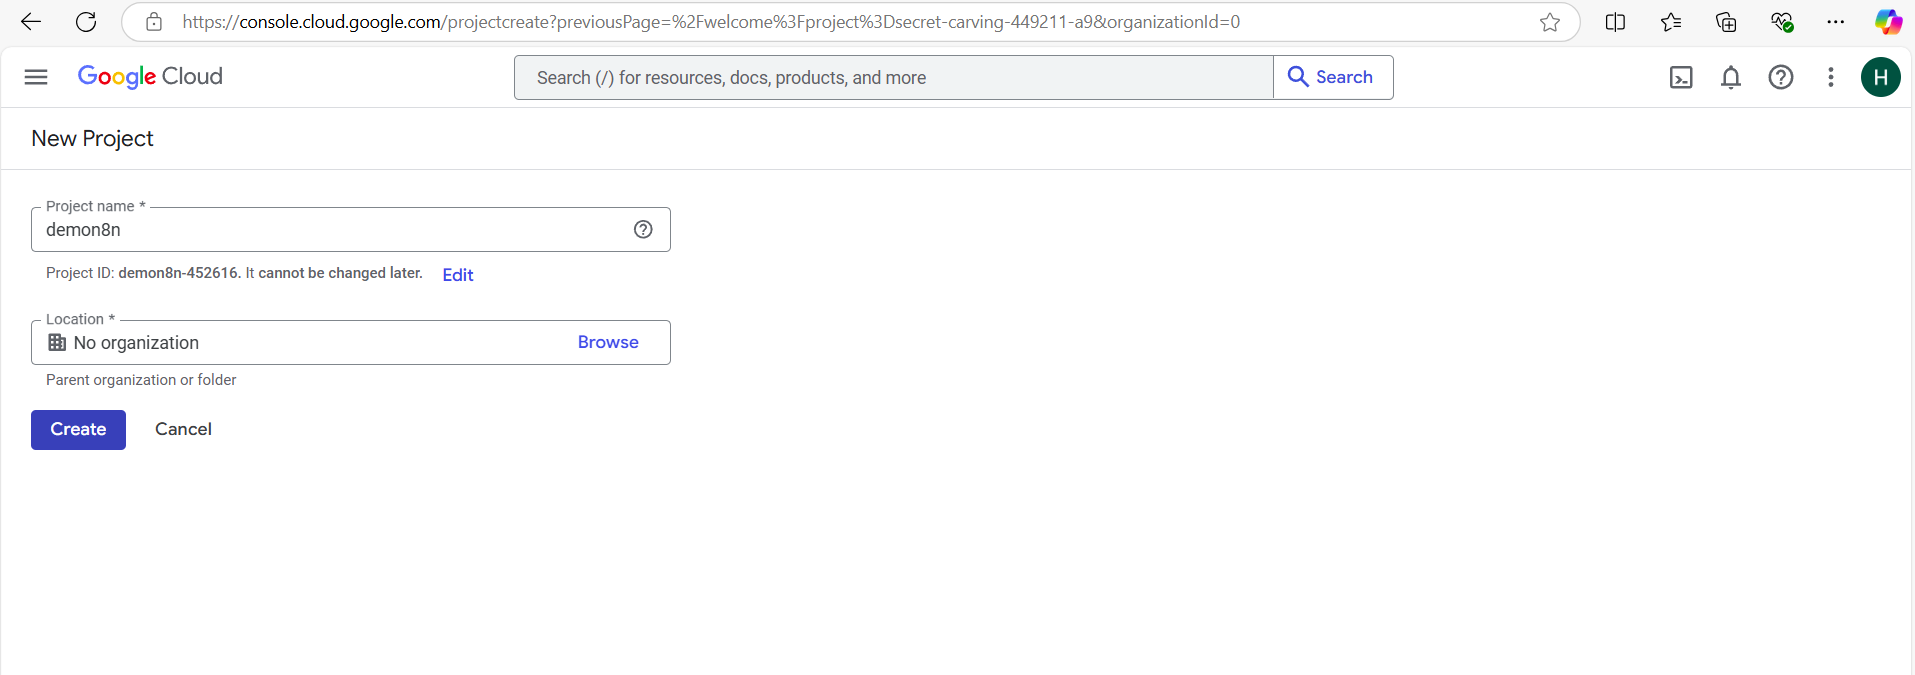
\includegraphics[width=0.95\textwidth]{images/GGcloud-1.png}
    
    \end{figure}
    
    \begin{figure}[H]
    \centering
    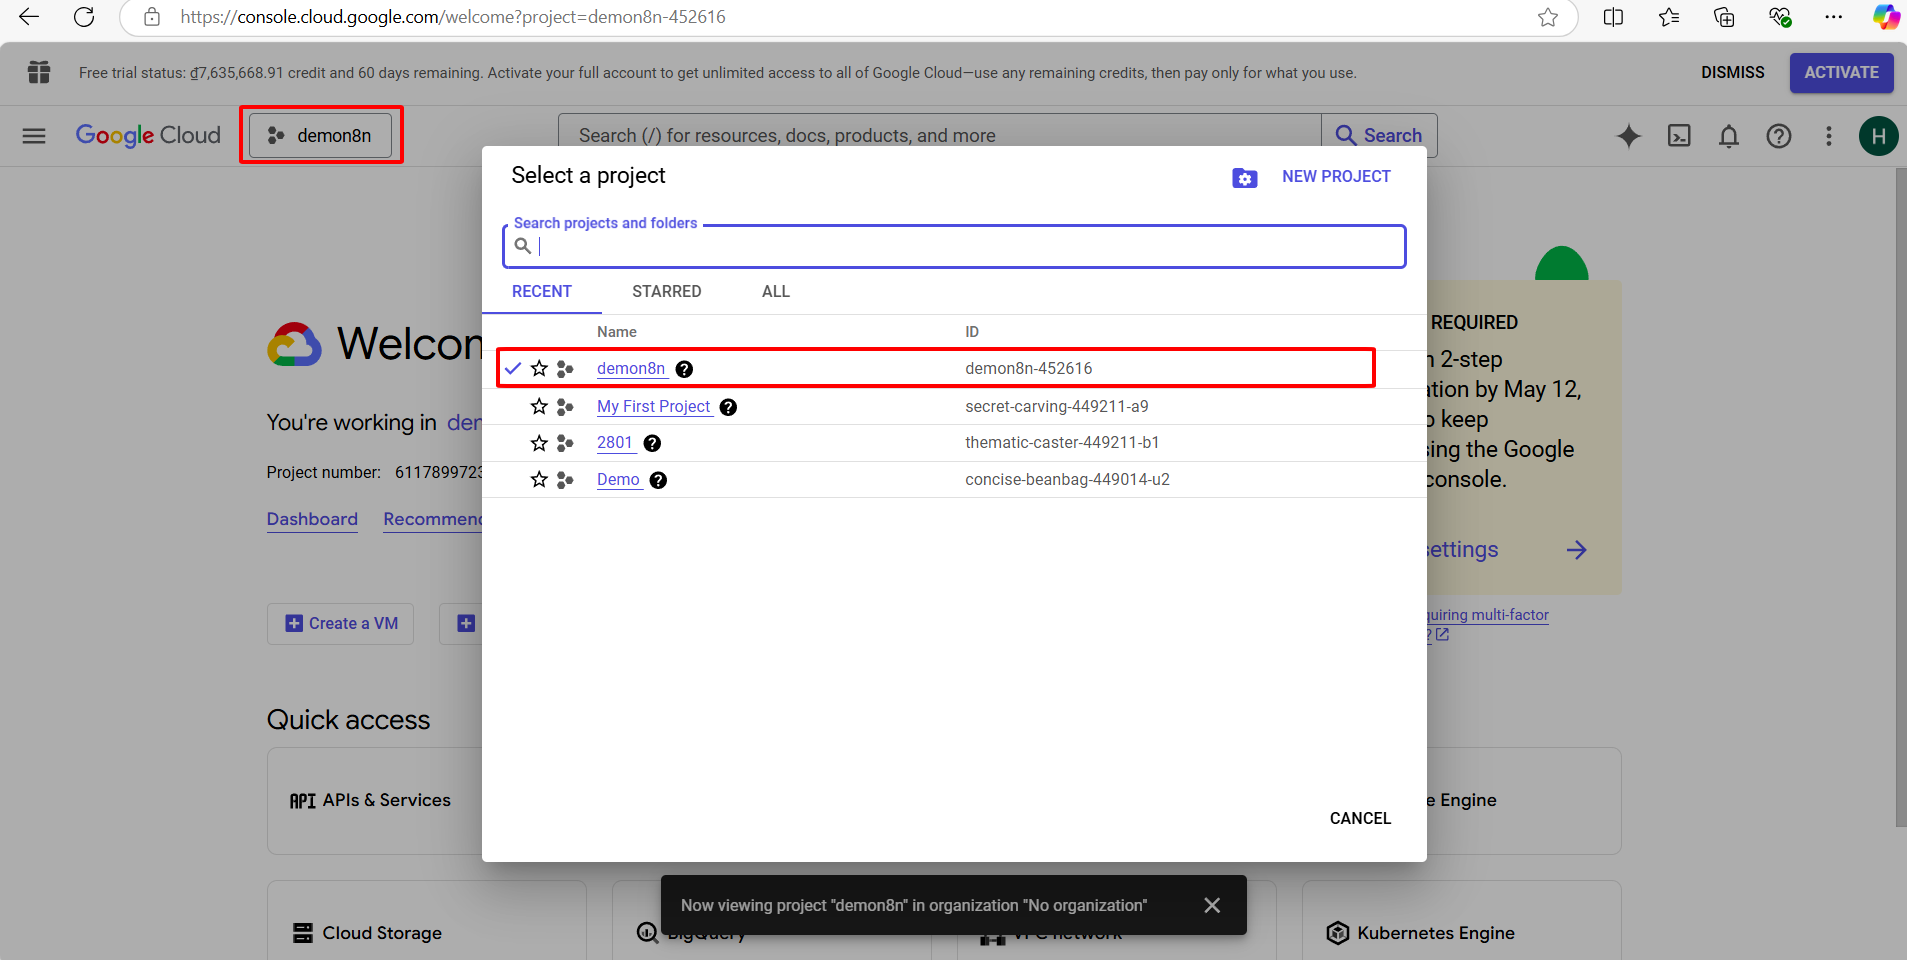
\includegraphics[width=0.95\textwidth]{images/GGcloud-2.png}
    
    \end{figure}
    \begin{figure}[H]
    \centering
    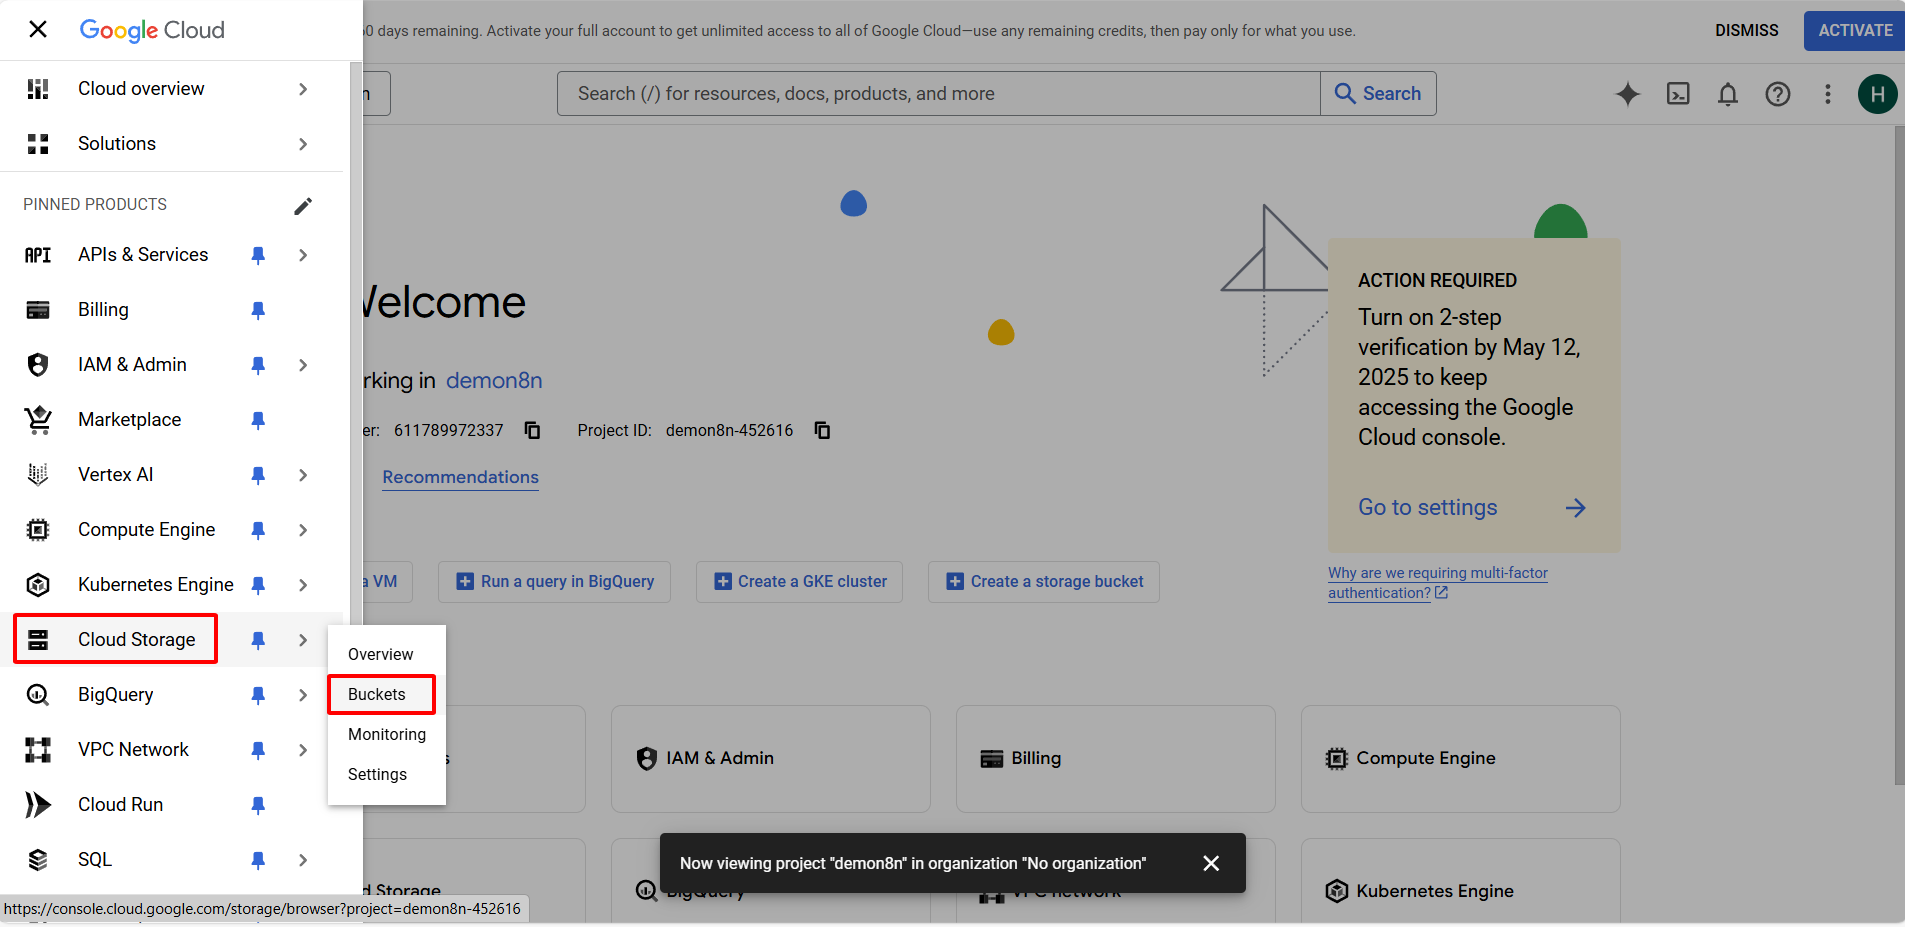
\includegraphics[width=0.95\textwidth]{images/GGcloud-3.png}

    \end{figure}
    \begin{figure}[H]
    \centering
    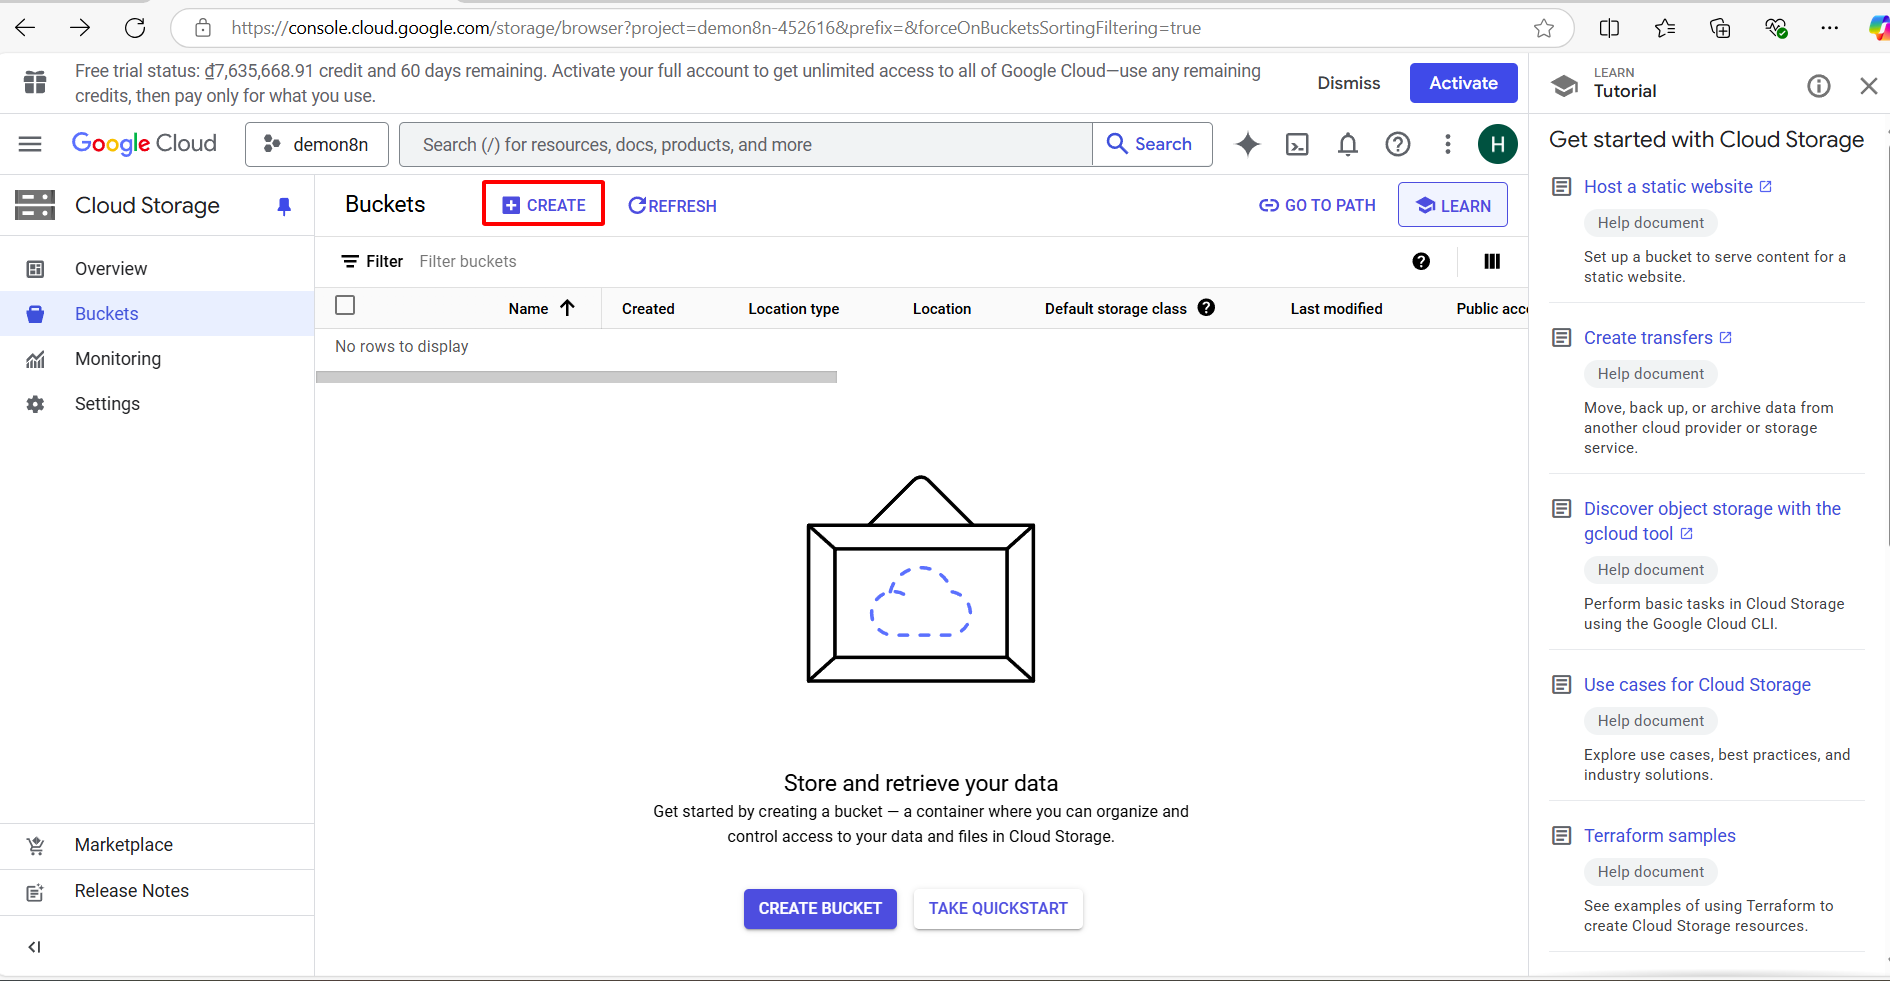
\includegraphics[width=0.95\textwidth]{images/GGcloud-4.png}
    
    \end{figure}
    \begin{figure}[H]
    \centering
    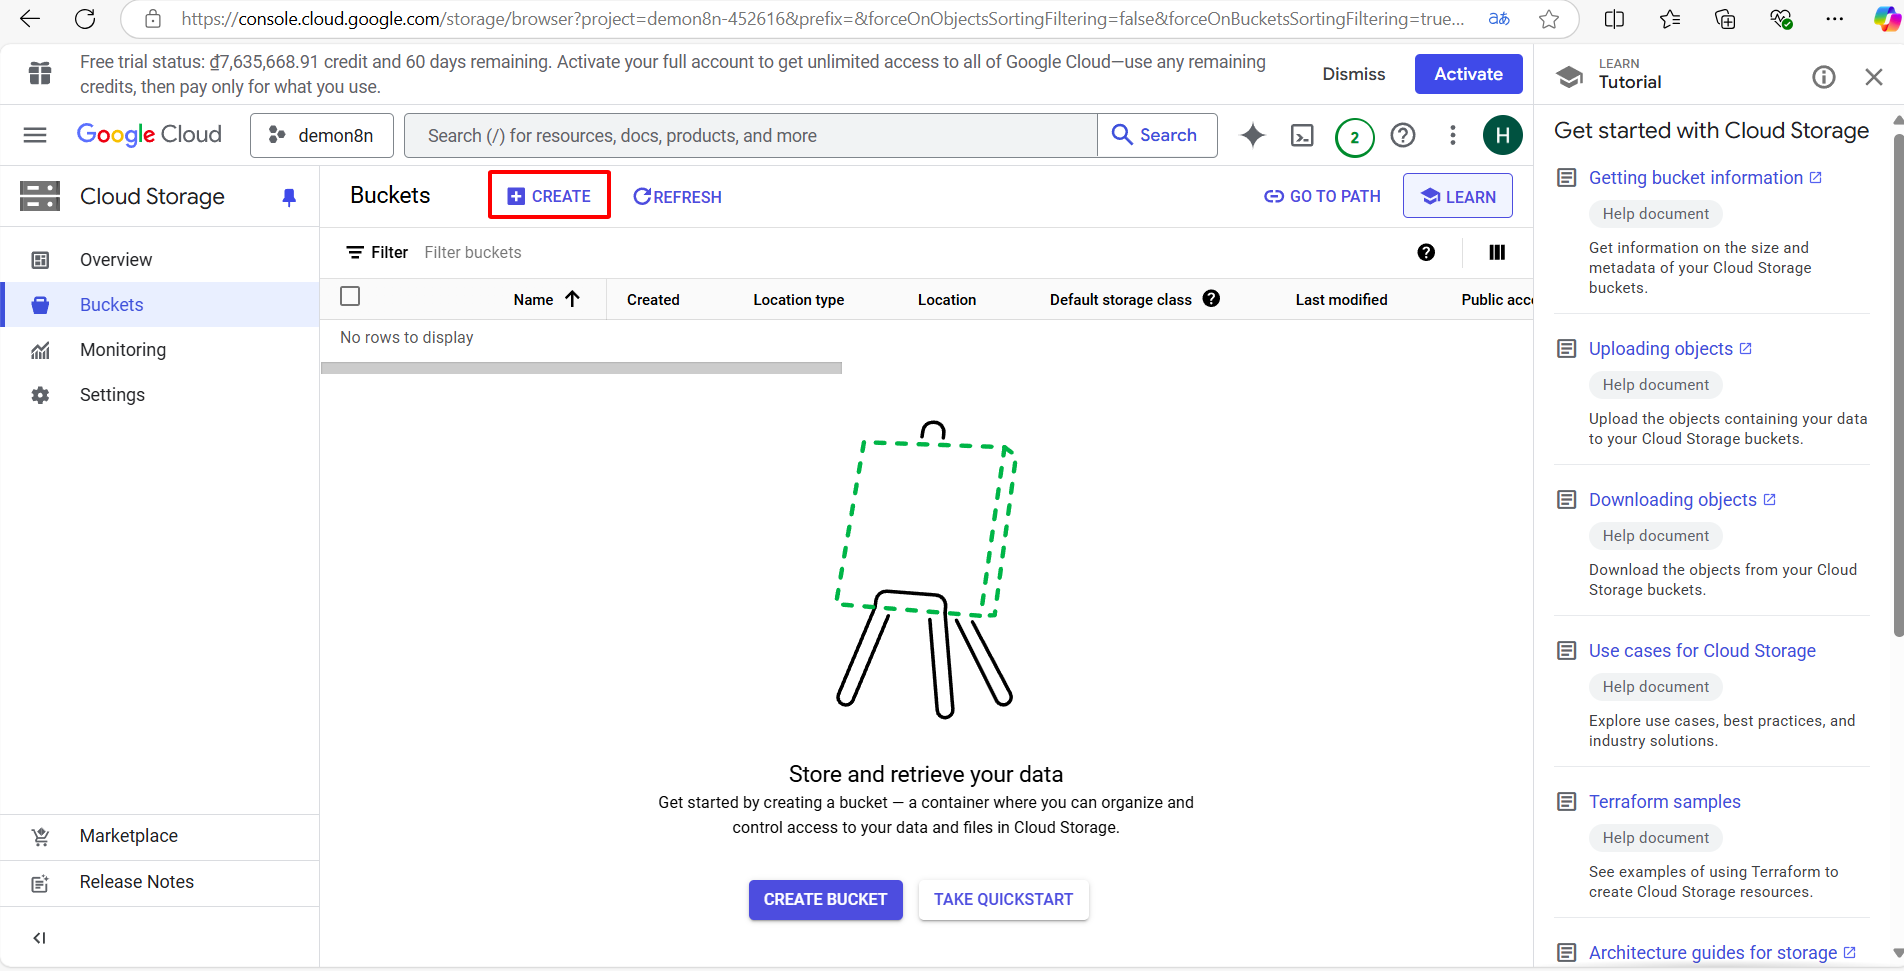
\includegraphics[width=0.95\textwidth]{images/GGcloud-5.png}
    
    \end{figure}
    \begin{figure}[H]
    \centering
    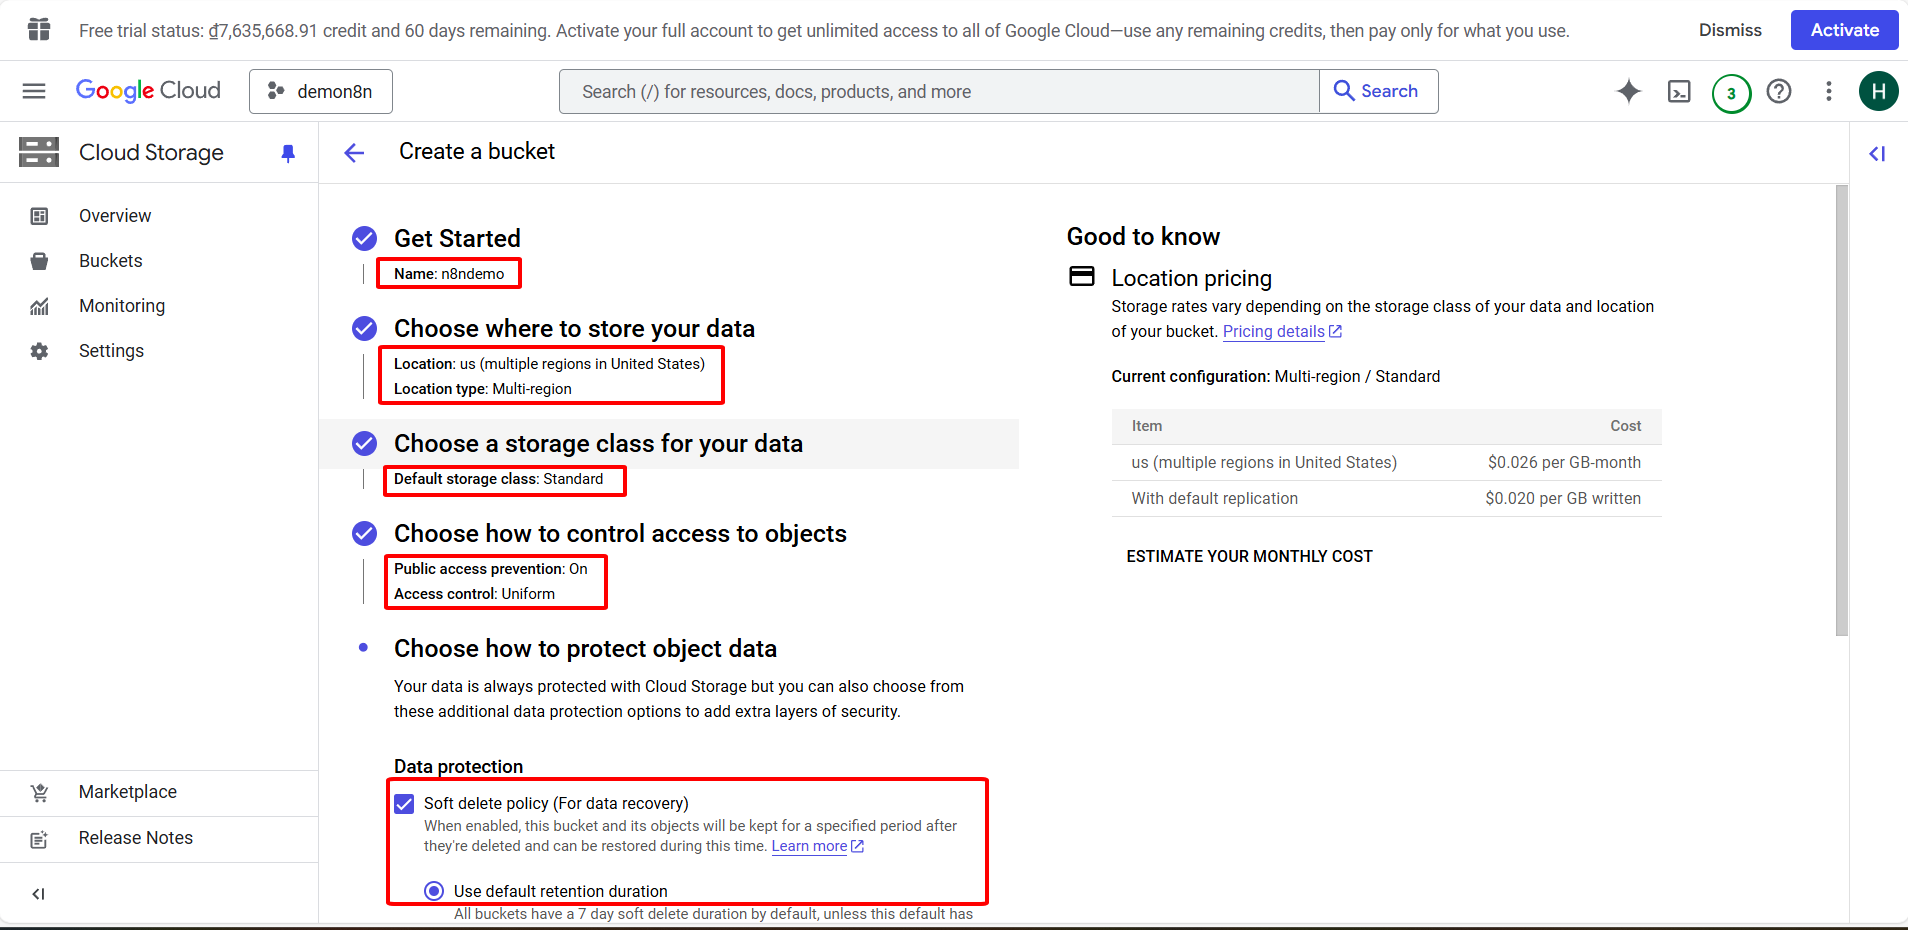
\includegraphics[width=0.95\textwidth]{images/GGcloud-6.png}
    
    \end{figure}
    \begin{figure}[H]
    \centering
    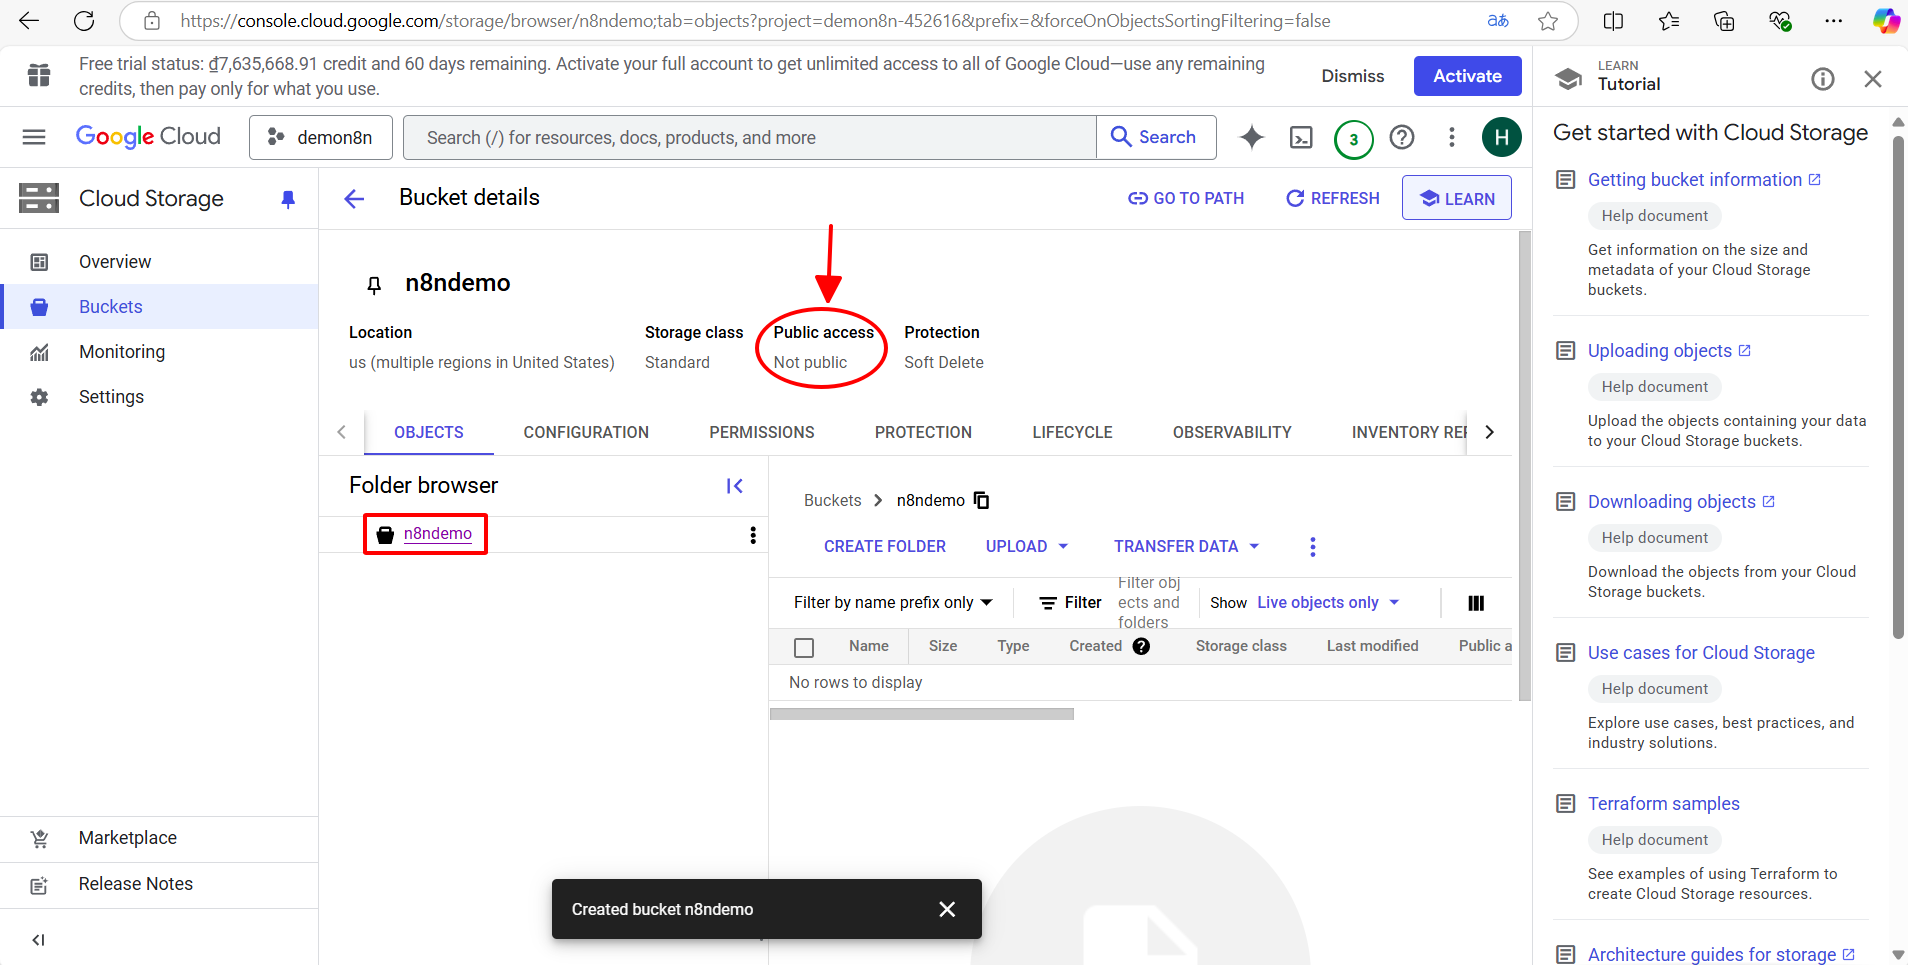
\includegraphics[width=0.95\textwidth]{images/GGcloud-7.png}
    
    \end{figure}
    \begin{figure}[H]
    \centering
    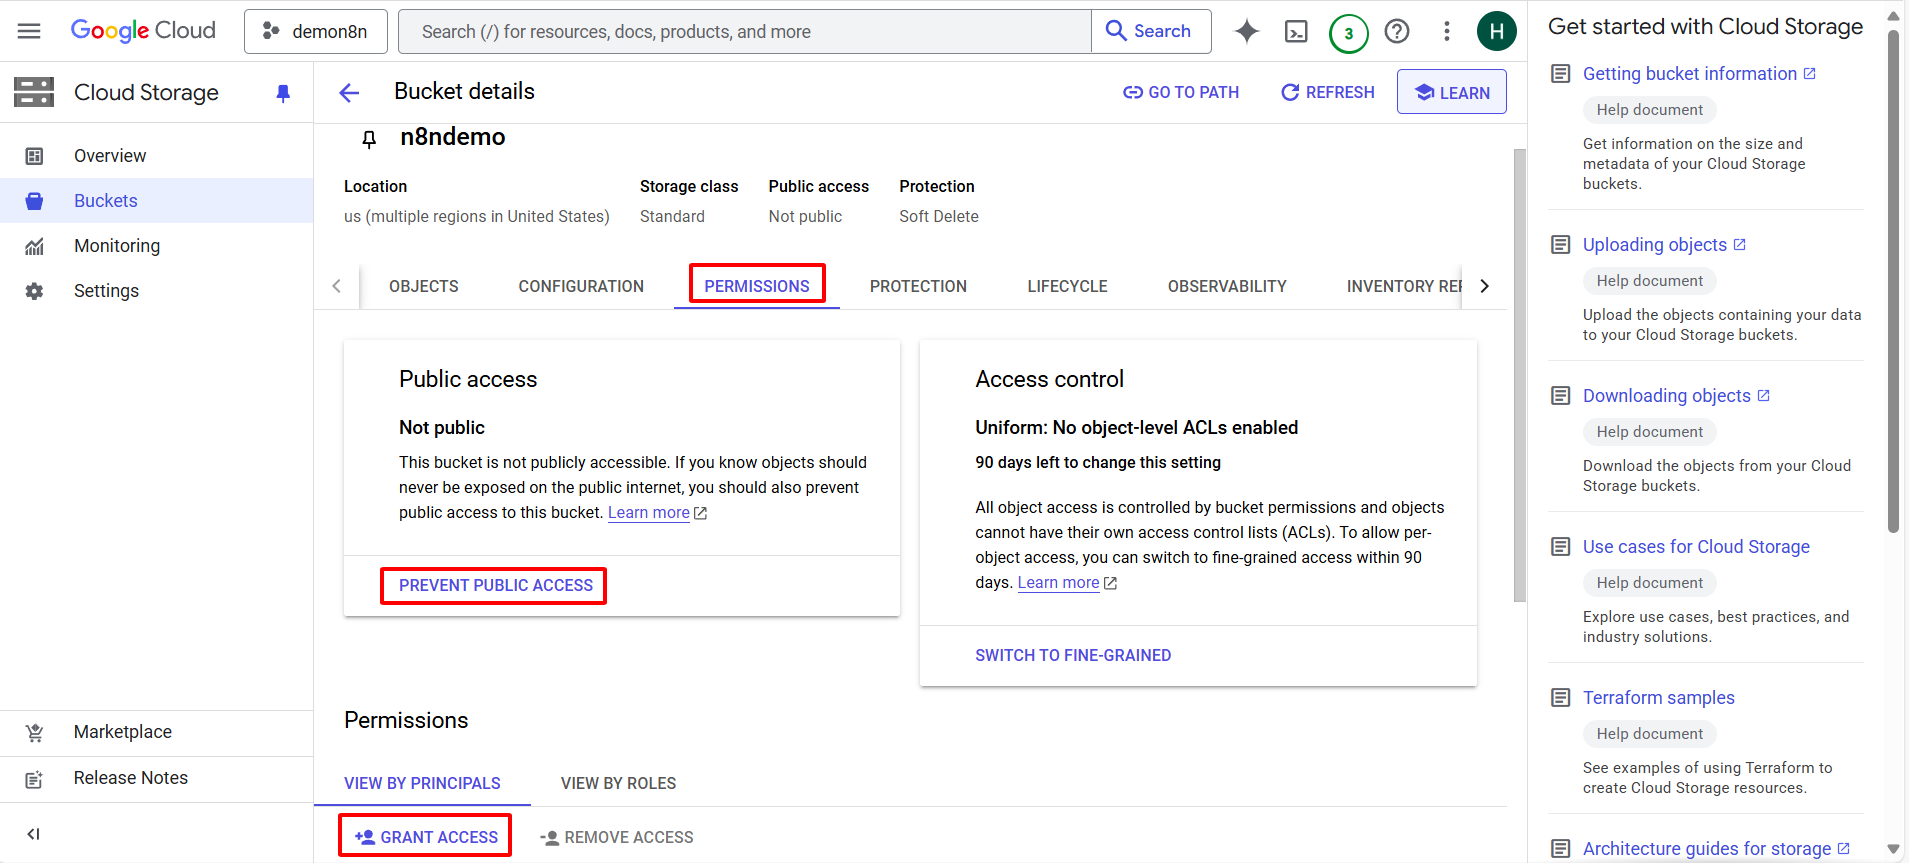
\includegraphics[width=0.95\textwidth]{images/GGcloud-8.png}
    
    \end{figure}
    \begin{figure}[H]
    \centering
    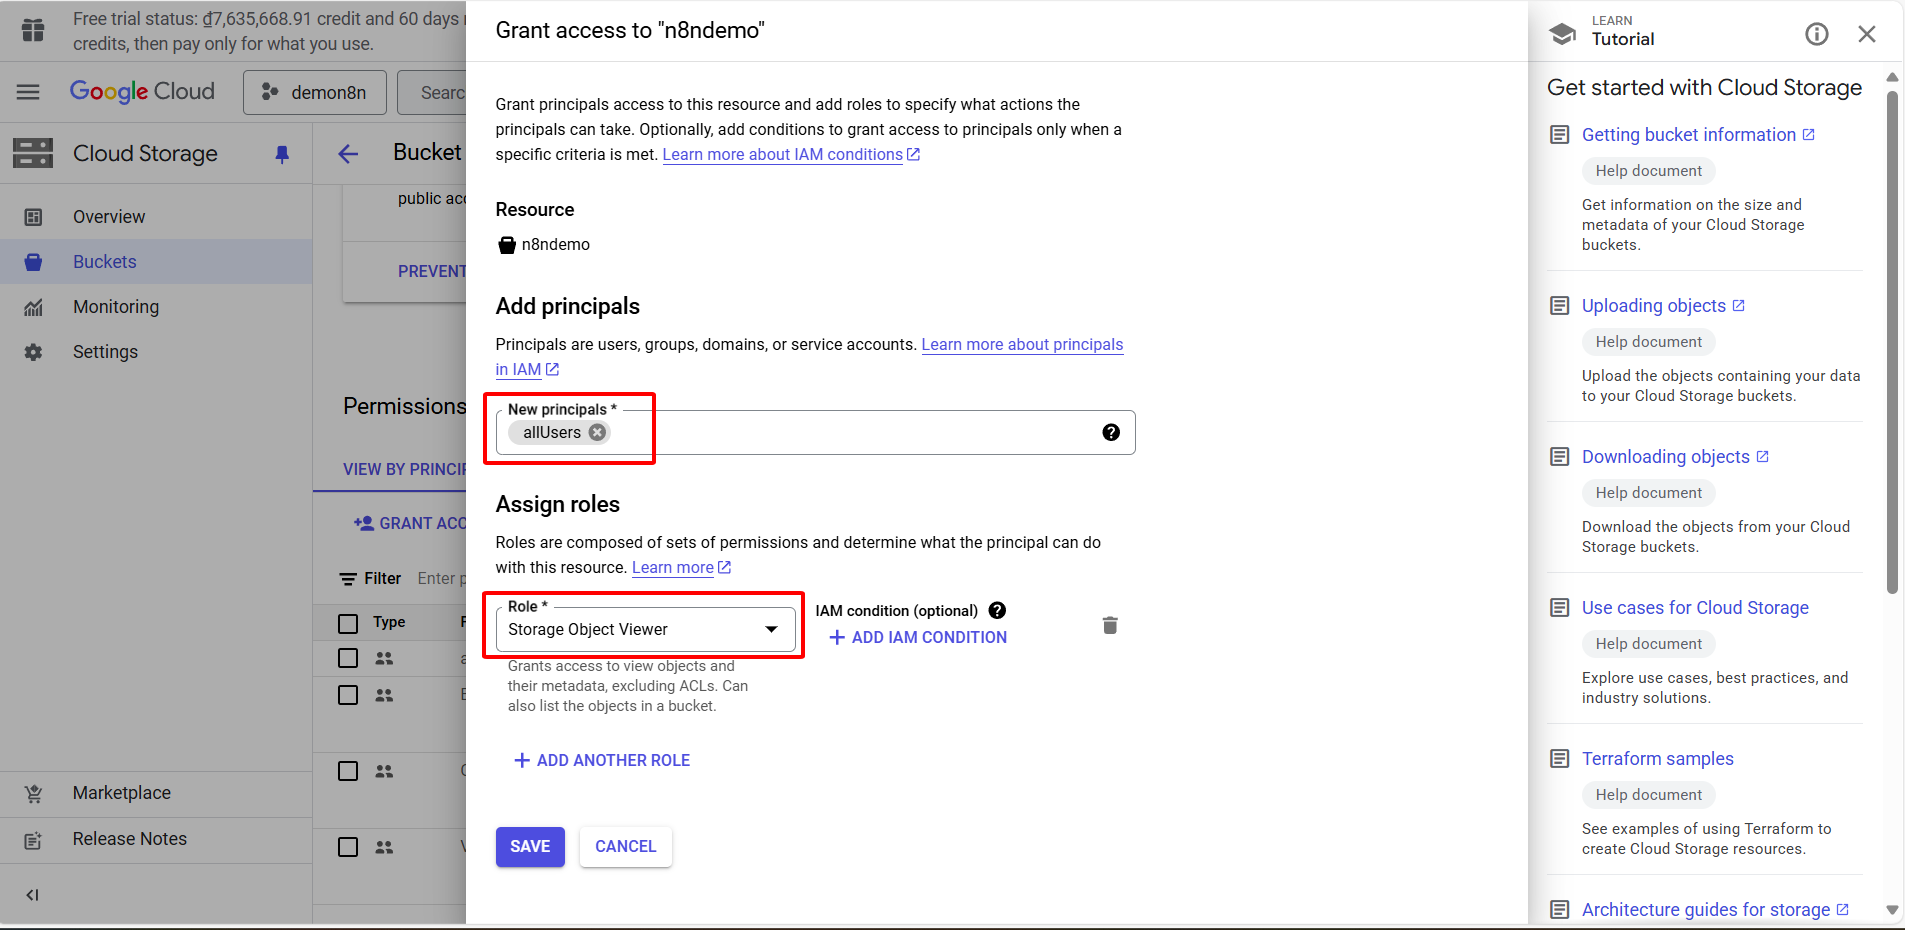
\includegraphics[width=0.95\textwidth]{images/GGcloud-9.png}
    
    \end{figure}
    \begin{figure}[H]
    \centering
    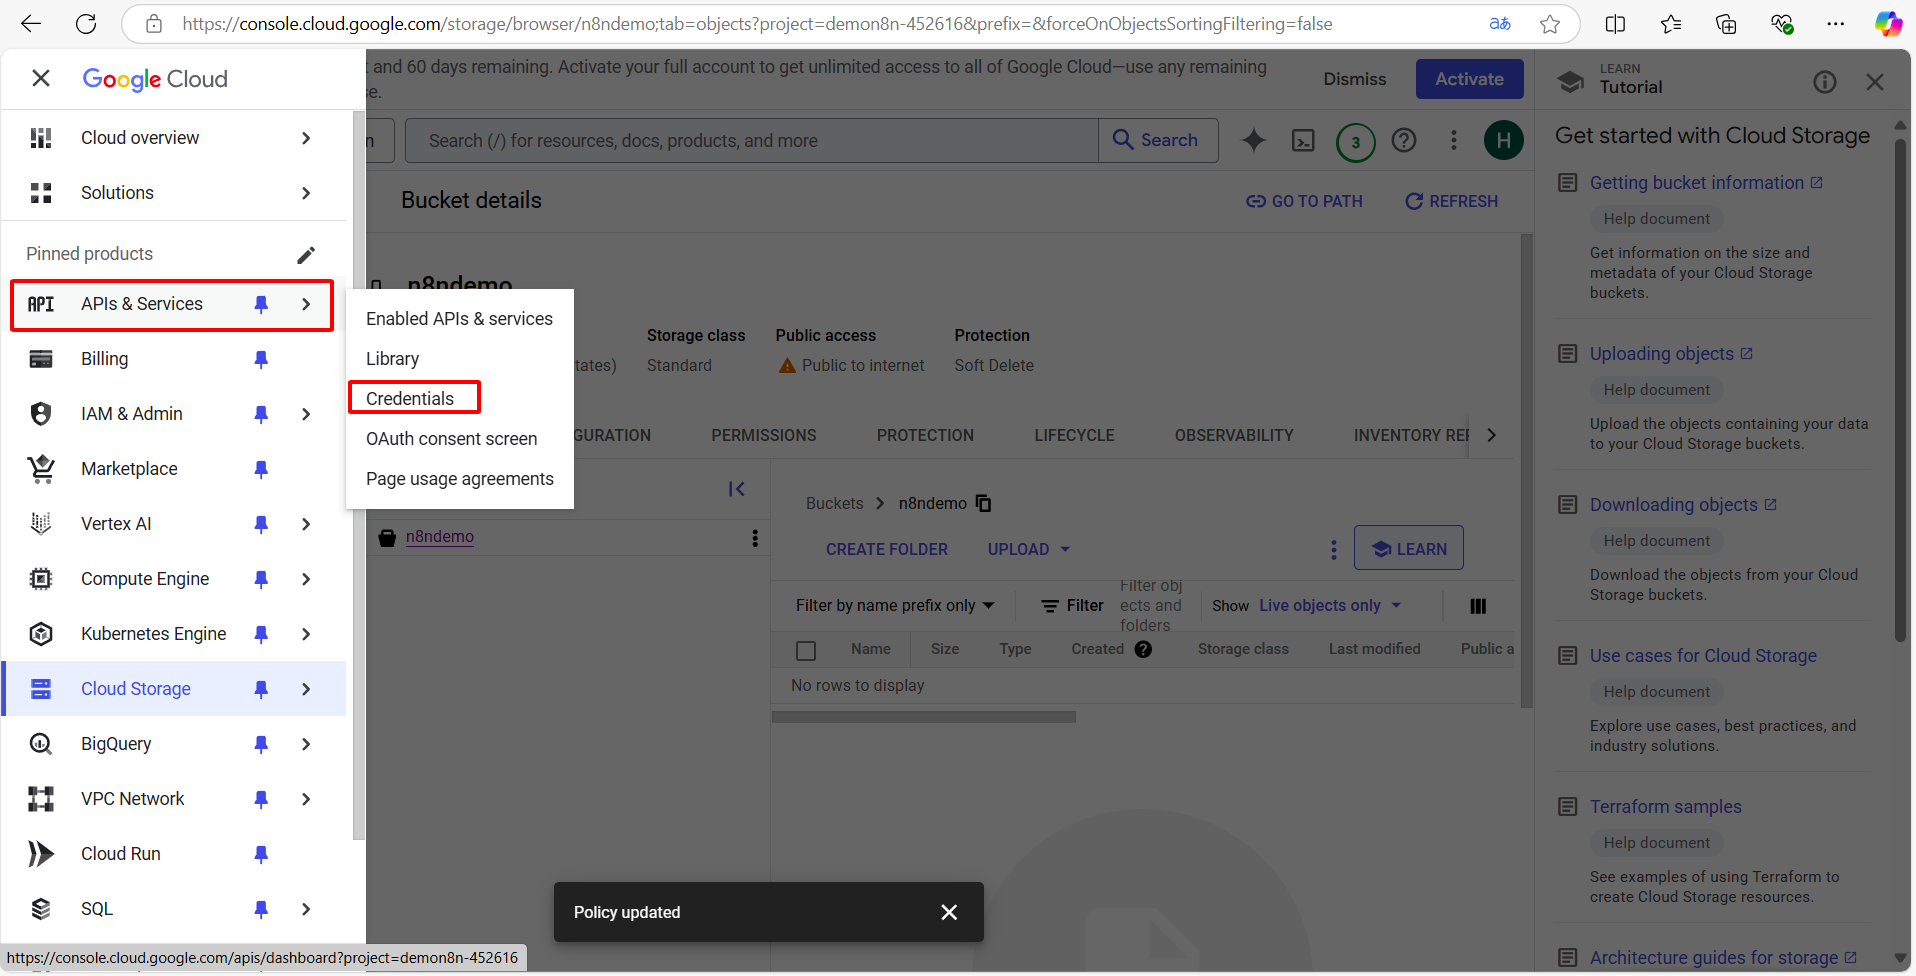
\includegraphics[width=0.95\textwidth]{images/GGcloud-10.png}
    
    \end{figure}
        \begin{figure}[H]
    \centering
    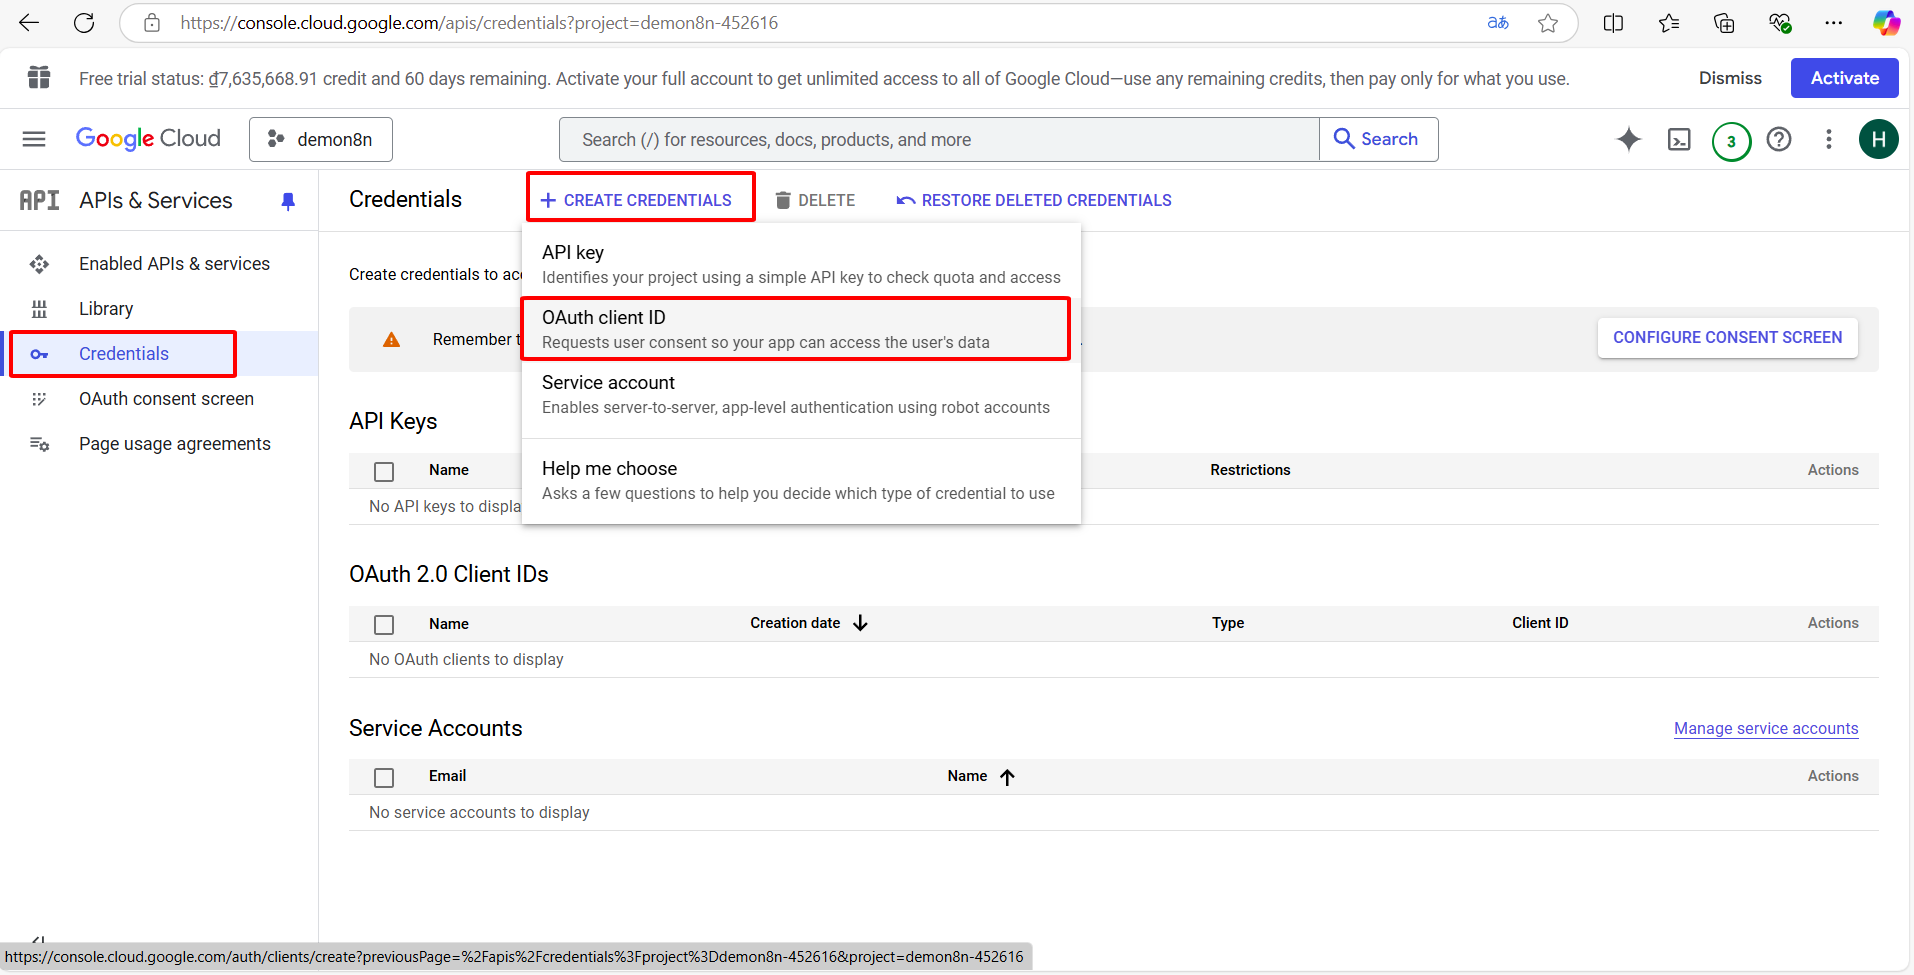
\includegraphics[width=0.95\textwidth]{images/GGcloud-11.png}
    
    \end{figure}
    \begin{figure}[H]
    \centering
    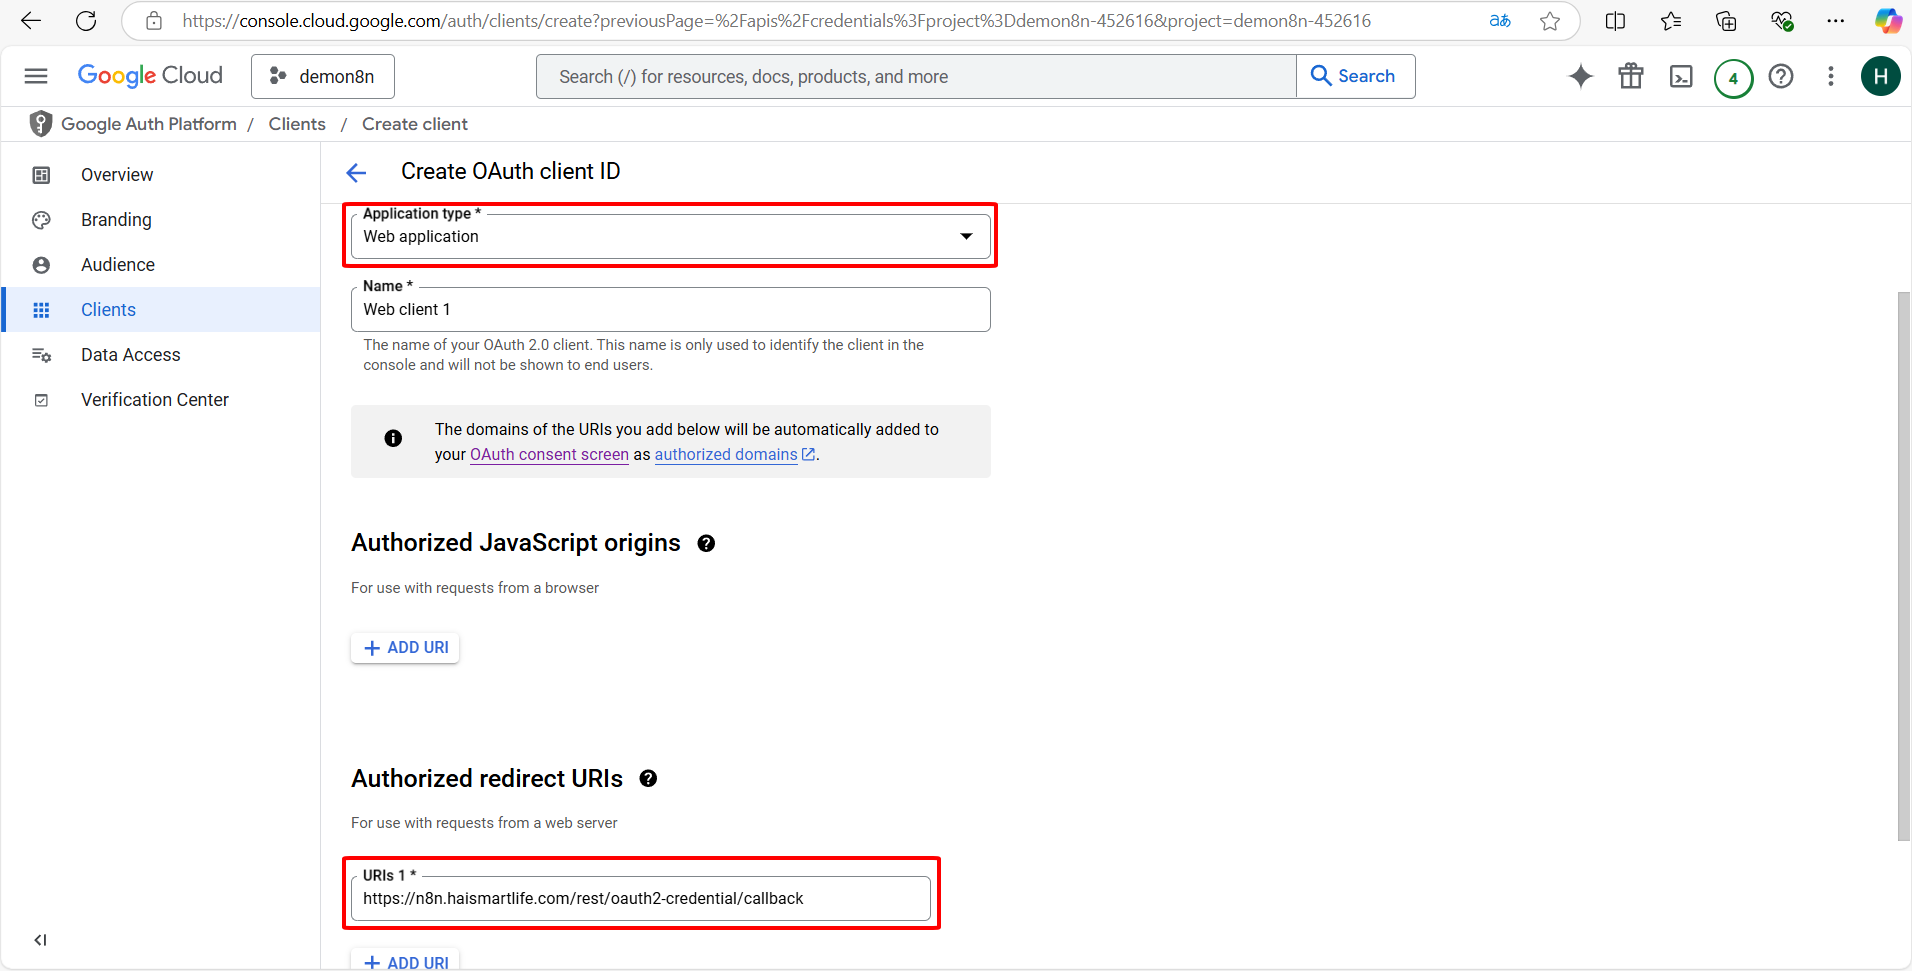
\includegraphics[width=0.95\textwidth]{images/GGcloud-12.png}
    
    \end{figure}

    \begin{figure}[H]
    \centering
    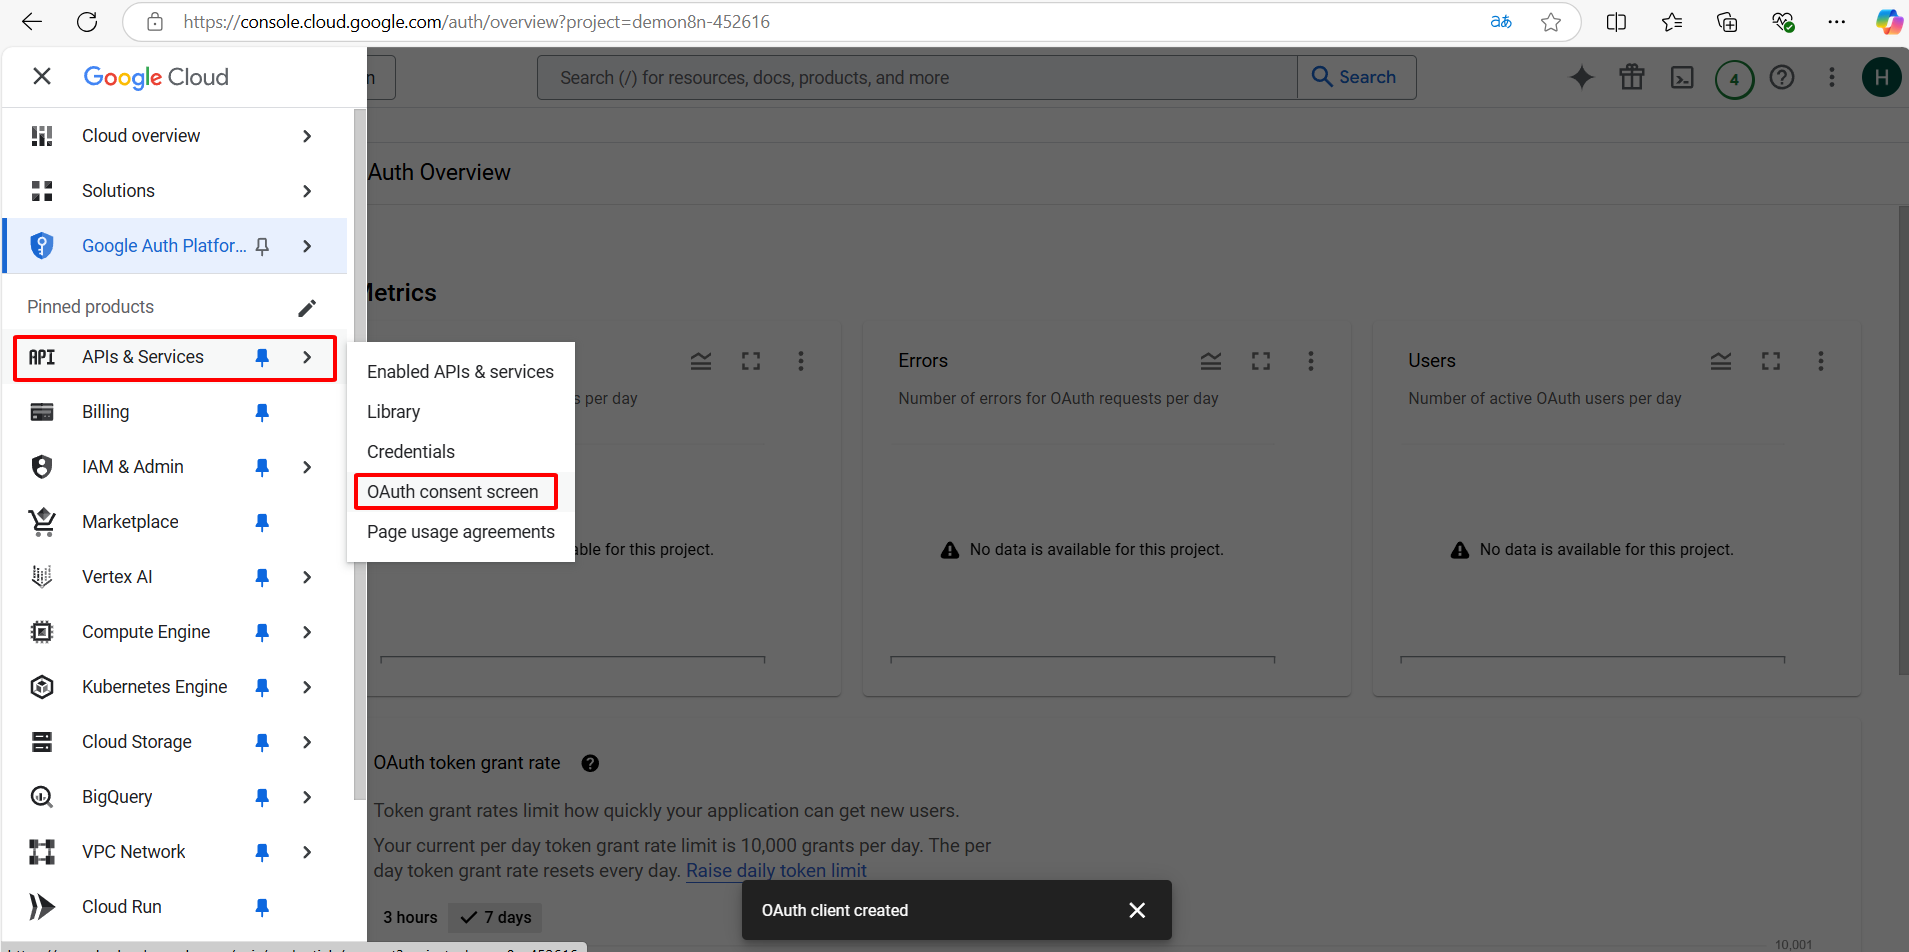
\includegraphics[width=0.95\textwidth]{images/GGcloud-14.png}
    
    \end{figure}
    \begin{figure}[H]
    \centering
    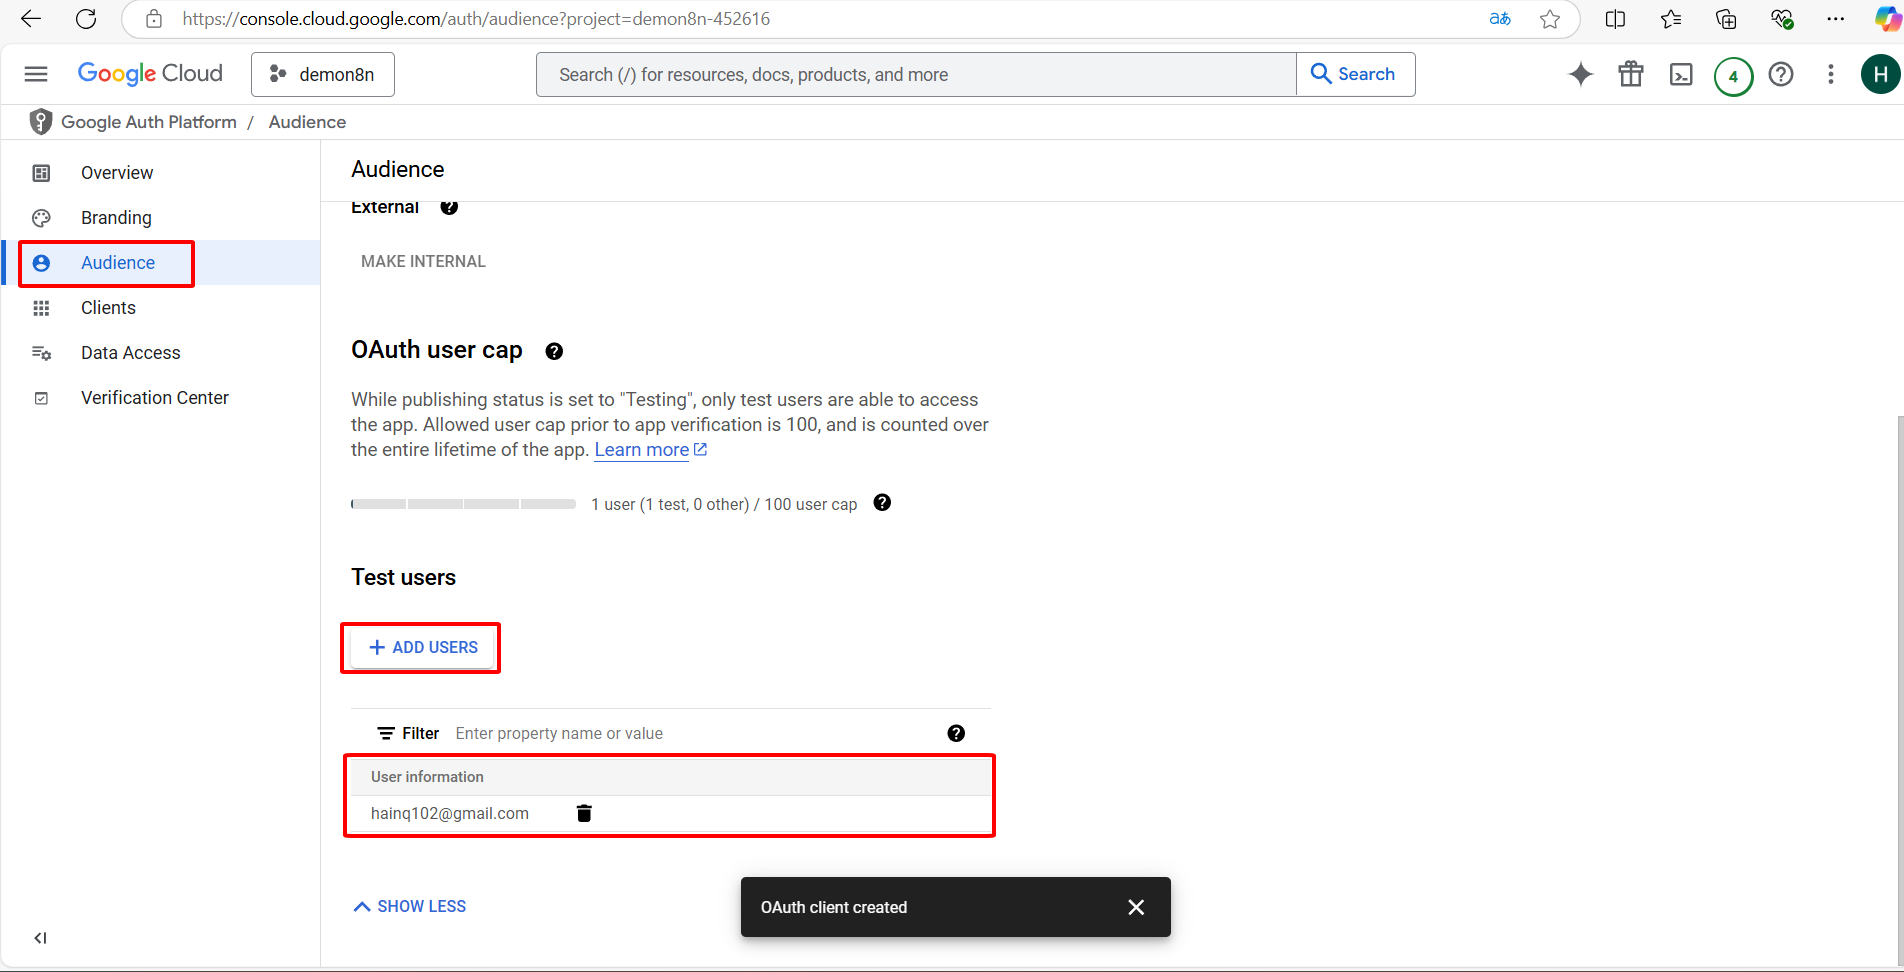
\includegraphics[width=0.95\textwidth]{images/GGcloud-15.png}
    
    \end{figure}

    \begin{figure}[H]
    \centering
    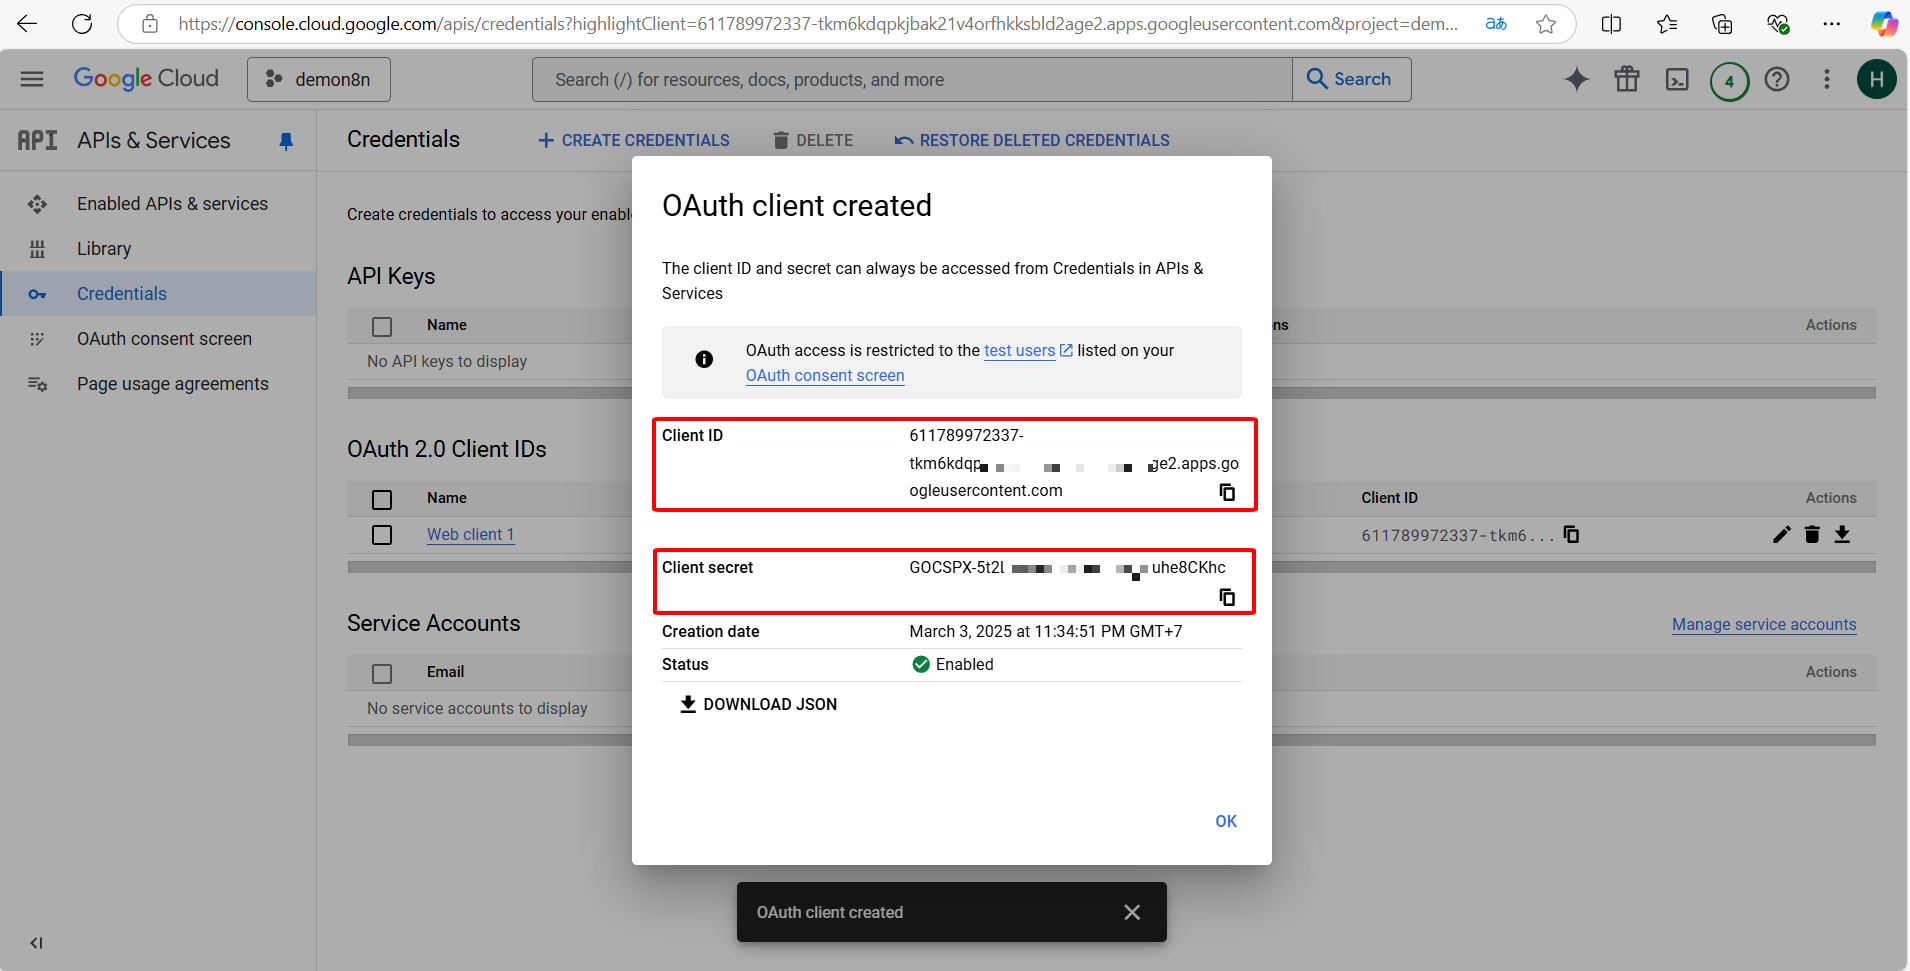
\includegraphics[width=0.95\textwidth]{images/GGcloud-13.png}
    
    \end{figure}


    
    \item \textbf{Bước 2: Tạo node "Google cloud storage" trong n8n}\\
    \begin{figure}[H]
    \centering
    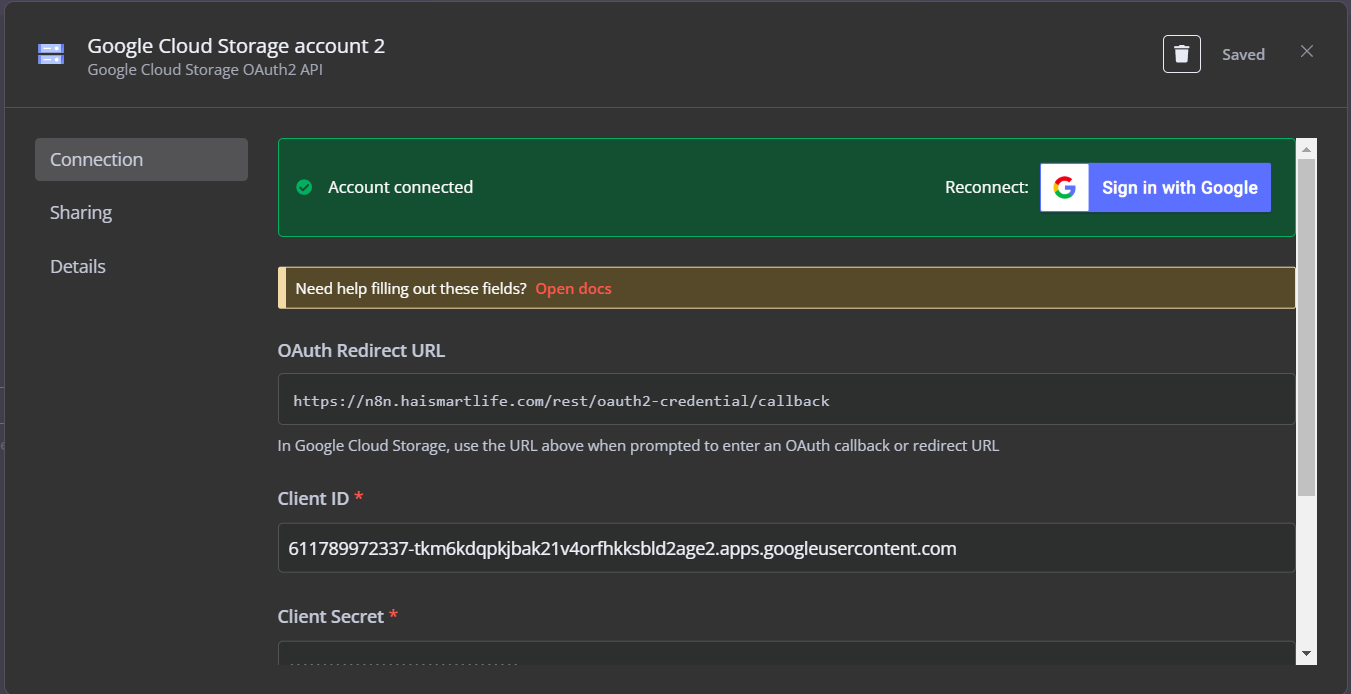
\includegraphics[width=0.95\textwidth]{images/GGcloud-16.png}
    
    \end{figure}
    
 Tạo Node HTTP trong n8n, trong phần Header Auth chúng ta tạo credential như hình trên:\\
 Name: authorization\\
 Value: API vừa copy ở web Together AI\\
     \begin{figure}[H]
    \centering
    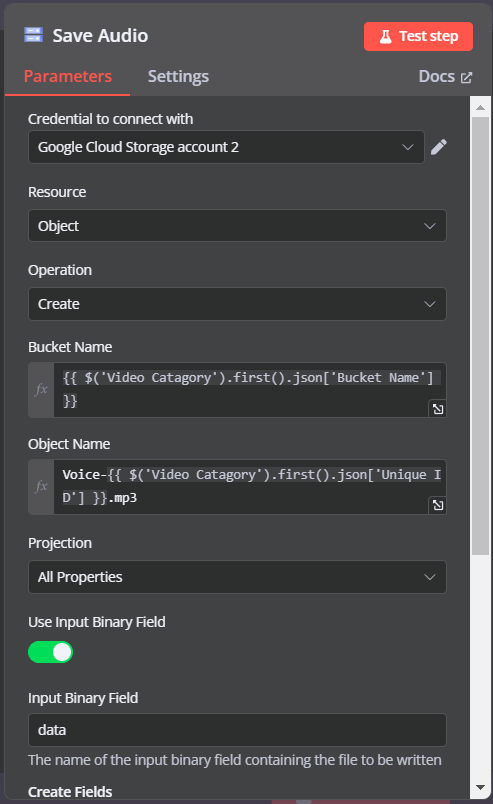
\includegraphics[width=0.6\textwidth]{images/GGcloud-17.png}
    
    \end{figure}
       \verb|{{ $('Video Catagory').first().json['Bucket Name'] }}|\\
    \verb|Voice-{{ $('Video Catagory').first().json['Unique ID'] }}.mp3|

\end{itemize}

%---------------------------------
\subsection{Hailuo AI - Tạo video bằng Hailuo AI.}
\begin{itemize}[label=]
    \item \textbf{Bước 1: Tạo API key Hailuo AI} 
    
    Truy cập vào link \url{https://hailuoai.video/} \\ 
    Tìm đến API keys và copy nó ta sẽ được dãy ký tự.\\
    Lưu ý: Thêm thông tin thẻ thanh toán và sử dụng như thường, và có thể thay node này bằng node khác có chức năng tương đương thể thử.\\
    
    \begin{figure}[H]
    \centering
    \includegraphics[width=0.95\textwidth]{images/HailuoAI.png}
    \caption{Tạo API Together AI}
    
    \end{figure}
    \item \textbf{Bước 2: Tạo node "HTTP truy cập Together AI" trong n8n}\\
    \begin{figure}[H]
    \centering
    \includegraphics[width=0.95\textwidth]{images/HailuoAI-1.png}
    \caption{Tạo API Elevenlabs}
    
    \end{figure}
    \begin{figure}[H]
    \centering
    \includegraphics[width=0.95\textwidth]{images/HailuoAI-2.png}
    \caption{Tạo API Elevenlabs}
    
    \end{figure}
    
 Tạo Node HTTP trong n8n, trong phần Header Auth chúng ta tạo credential như hình trên:\\
 Name: authorization\\
 Value: Bearer API vừa copy ở web Together AI\\
 

Tại mục URL nhập: \\
"https://api.together.xyz/v1/chat/completions"\\

Tại mục Json nhập: 


Dưới đây là đoạn JSON:\\

Nơi lấy code \url{https://haismartlife.com/}


\end{itemize}


%---------------------------------
\subsection{Andynocode - Combine video.}
\begin{itemize}[label=]
    \item \textbf{Bước 1: Tạo API key Hailuo AI} 
    
    Truy cập vào link \url{https://hailuoai.video/} \\ 
    Tìm đến API keys và copy nó ta sẽ được dãy ký tự.\\
    Lưu ý: Thêm thông tin thẻ thanh toán và sử dụng như thường, và có thể thay node này bằng node khác có chức năng tương đương thể thử.\\
    
    \begin{figure}[H]
    \centering
    \includegraphics[width=0.95\textwidth]{images/Andy02.png}
    \caption{Tạo API Together AI}
    
    \end{figure}
    \item \textbf{Bước 2: Tạo node "HTTP truy cập Together AI" trong n8n}\\
    \begin{figure}[H]
    \centering
    \includegraphics[width=0.95\textwidth]{images/Andy01.png}
    \caption{Tạo API Elevenlabs}
    
    \end{figure}

    
 Tạo Node HTTP trong n8n, trong phần Header Auth chúng ta tạo credential như hình trên:\\
 Name: authorization\\
 Value: Bearer API vừa copy ở web Together AI\\
 

Tại mục URL nhập: \\
"https://api.together.xyz/v1/chat/completions"\\

Tại mục Json nhập: 


Dưới đây là đoạn JSON:\\

Nơi lấy code \url{https://haismartlife.com/}


\end{itemize}


% % % Chương 10
 \chapter{Case Study thực tế (phần 2)}

\section{\textbf{Dự án 1: Tạo RAG system - hệ thống trả lời câu hỏi bằng tài liệu người dùng}}

\href{https://drive.google.com/file/d/1SwPcQe6HypodnICqbvVpzWVUKQA8_PLI/view?usp=sharing}{\textbf{\underline {Link tải workflow}}}

\begin{figure}[H]
    \centering
    \includegraphics[width=1\textwidth]{images/1rag01.pdf}
    \caption{Workflow kết quả dự án 1}

\end{figure}

Workflow trong mã nguồn được chia sẻ là một hệ thống RAG (Retrieval Augmented Generation) nâng cao được xây dựng trên nền tảng n8n. Đây là một giải pháp toàn diện cho việc xử lý, lưu trữ và truy vấn thông tin từ nhiều loại tài liệu khác nhau.

\textbf{Chức năng chính:}
\begin{itemize}
    \item \textbf{Tự động xử lý tài liệu:} Phát hiện khi tài liệu mới được tạo hoặc cập nhật trong thư mục Google Drive; Hỗ trợ nhiều định dạng tài liệu: PDF, Google Docs, CSV, Excel, và văn bản thông thường; Tự động trích xuất nội dung từ các loại tài liệu khác nhau.
    
    \item \textbf{Xử lý thông minh dựa trên loại tài liệu:} Văn bản và PDF: Chia nhỏ thành các đoạn có nghĩa, tạo embedding và lưu vào Supabase; Dữ liệu bảng (CSV/Excel): Trích xuất cấu trúc và nội dung, lưu trữ thông tin metadata và dữ liệu hàng.
    
    \item \textbf{Lưu trữ dữ liệu hiệu quả:} Sử dụng bảng \texttt{documents} với vectơ embedding thông qua pgvector; Bảng \texttt{document\_metadata} lưu thông tin về tài liệu; Bảng \texttt{document\_rows} lưu dữ liệu từ các tệp CSV/Excel.
    
    \item \textbf{Giao diện trò chuyện AI thông minh:} API webhook để nhận yêu cầu từ người dùng; Agent AI có thể sử dụng nhiều công cụ khác nhau để trả lời câu hỏi; Hỗ trợ bộ nhớ trò chuyện qua PostgreSQL.
    
    \item \textbf{Khả năng truy vấn đa dạng:} Tìm kiếm tương tự ngữ nghĩa (RAG); Truy vấn SQL trực tiếp trên dữ liệu bảng; Truy xuất toàn bộ nội dung tài liệu khi cần thiết.
\end{itemize}

\textbf{Điểm nổi bật:}
\begin{itemize}
    \item \textbf{Kiến trúc RAG Agent thông minh:} Không chỉ đơn thuần là RAG thông thường, workflow này sử dụng cách tiếp cận "agent" cho phép LLM chọn công cụ phù hợp nhất để trả lời câu hỏi.
    
    \item \textbf{Xử lý tài liệu linh hoạt:} Tự động phát hiện định dạng tài liệu và áp dụng phương pháp xử lý phù hợp, không cần cấu hình riêng cho từng loại tài liệu.
    
    \item \textbf{Tối ưu cho dữ liệu số học:} Sử dụng SQL để thực hiện phân tích chính xác trên dữ liệu bảng, khắc phục hạn chế của RAG tiêu chuẩn với dữ liệu số học.
    
    \item \textbf{Khả năng mở rộng:} Thiết kế dễ dàng mở rộng để hỗ trợ thêm nguồn dữ liệu và công cụ mới.
    
    \item \textbf{Hiệu quả lưu trữ:} Sử dụng JSONB trong Supabase để lưu trữ dữ liệu bảng mà không cần tạo bảng mới cho mỗi tệp CSV.
    
    \item \textbf{Tận dụng công nghệ hiện đại:} Kết hợp pgvector, OpenAI Embeddings, và LLM để tạo hệ thống RAG hoàn chỉnh.
\end{itemize}

\textbf{Hướng dẫn thiết lập:}

\textit{Bước 1: Chuẩn bị cơ sở dữ liệu}
\begin{itemize}
    \item \textbf{Thiết lập Supabase:} Tạo tài khoản Supabase và dự án mới; Lưu thông tin kết nối: URL và API Key.
    \begin{figure}[H]
    \centering
    \includegraphics[width=1\textwidth]{images/1rag05.pdf}
    \caption{Thông tin Credential của Supabase}
    \end{figure}
    
    \item \textbf{Thiết lập PostgreSQL:} Đảm bảo PostgreSQL được cài đặt và hỗ trợ pgvector; Chạy các node tạo bảng theo thứ tự: \texttt{Create Documents Table and Match Function}, \texttt{Create Document Metadata Table}, \texttt{Create Document Rows Table}. Chạy 3 node này để tạo bảng và gọi thư viện tạo vector trong Supabase.\\
    \begin{figure}[H]
\centering
\includegraphics[width=1\textwidth]{images/1rag06.pdf}
\caption{Thông tin Credential của Postgres}
\end{figure}
Password của Postgres chính là mật khẩu lúc khởi tạo dự án. Nếu quên mật khẩu có thể vào cài đặt - Database - Database password và đặt lại. \\

Luu ý: phải chạy 3 node postgres trước khi upload file lên googledrive, để tạo bảng và khởi tạo biến vector trước. Nếu không sẽ bị lỗi và không chạy được\\

\end{itemize}
    

    
\begin{figure}[H]
\centering
\includegraphics[width=1\textwidth]{images/1rag07.pdf}
\caption{Thông tin Credential của Postgres}
\end{figure}
    
    

\textit{Bước 2: Cấu hình Google Drive}
\begin{itemize}
    \item \textbf{Thiết lập OAuth:} Tạo OAuth credentials trong Google Developer Console; Thêm thông tin xác thực vào n8n.
    
    \item \textbf{Cấu hình thư mục:} Tạo thư mục riêng để chứa tài liệu cho bot; Lấy ID thư mục và cấu hình trong các node \texttt{File Created} và \texttt{File Updated}.
\end{itemize}

\textit{Bước 3: Cấu hình OpenAI API}
\begin{itemize}
    \item \textbf{Tạo API key:} Đăng ký tài khoản và tạo API key từ OpenAI; Thêm thông tin xác thực vào n8n.
    
    \item \textbf{Cấu hình model:} Cấu hình mô hình embeddings (text-embedding-3-small); Cấu hình mô hình chat (gpt-4 hoặc tương tự).
\end{itemize}

\textit{Bước 4: Thiết lập Workflow}
\begin{itemize}
    \item \textbf{Xử lý tài liệu:} Cấu hình node trigger với ID thư mục Google Drive; Thiết lập các node xử lý tài liệu; Cấu hình node \texttt{Switch} để định tuyến luồng dữ liệu.
    
    \item \textbf{Vector embedding:} Cấu hình \texttt{Character Text Splitter} (chunk 1000 ký tự, overlap 100 ký tự); Cấu hình \texttt{Embeddings OpenAI1}; Thiết lập \texttt{Insert into Supabase Vectorstore}.
    
    \item \textbf{Xử lý dữ liệu bảng:} Cấu hình \texttt{Insert Table Rows}; Thiết lập \texttt{Update Schema for Document Metadata}.
    
    \item \textbf{AI Agent:} Cấu hình webhook; Thiết lập \texttt{RAG AI Agent} với system prompt; Cấu hình các công cụ; Thiết lập \texttt{Postgres Chat Memory}.
\end{itemize}

\textit{Bước 5: Tích hợp giao diện người dùng}
\begin{itemize}
    \item \textbf{Thiết lập webhook:} Lấy URL webhook từ node \texttt{Webhook1}; Cấu hình API endpoint trong ứng dụng frontend - Lovable.dev để tạo giao diện frontend.
    
    \begin{figure}[H]
    \centering
    \includegraphics[width=1\textwidth]{images/1rag02.pdf}
    \caption{Workflow giao diện web tương tác}
    \end{figure}
Đây là một kỹ thuật khá hay để tạo giao diện thân thiện với người dùng và cũng rất đơn giản để làm được.\\

\textbf{Step 1:} Truy cập web \url{https://lovable.dev/} - Đăng nhập và paste Prompt sau vào ô thoại của Lovable, trang web sẽ tự tạo frontend cho bạn (có thẻ tự thay đổi đổi có giao diện phù hợp mỗi người.

\textbf{Prompt:} \emph{Create a clean, modern AI chat interface similar to ChatGPT, but without the conversation history sidebar. The layout includes a top header bar with the text \textquotedblleft RAG AI AGENT \textquotedblright{} styled as a logo (bold, large font, center-aligned). Below that is the main chat area: a vertically scrolling window with alternating chat bubbles for user and assistant messages. Use soft shadows, large rounded corners (2xl), and a neutral background (\#f5f5f5). The input area is fixed at the bottom, containing an expanding text input and a \textquotedblleft Send\textquotedblright{} button with smooth animations. Typography is clean and sans-serif, with the assistant’s messages in a slightly dimmed color. Ensure mobile responsiveness and smooth message transitions.}\\

\textbf{Step 2:} Sau khi giao diện ban đầu được tạo thì tiếp tục nhập prompt chứa webhook n8n của bạn vào. Lưu ý URL này là của Production URL. \\

\textbf{Prompt:} \emph{
Khi tôi nhấn nút gửi thì dữ liệu đến webhook as a post request: nhập URL webhook của bạn}

$\Rightarrow$ Sau khi đã tạo xong giao diện web chúng ta cần publish nó lên như hình bên dưới. Như vậy các bạn đã tạo được một giao diện frontend kết nối với backend là n8n để thực hiện lệnh.
\end{itemize}    
    \begin{figure}[H]
    \centering
    \includegraphics[width=1\textwidth]{images/1rag03.pdf}
    \caption{Publish web để có thể truy cập bằng subdomain}
    \end{figure}
    


\textit{Bước 6: Kiểm thử và tối ưu}
\begin{itemize}
    \item \textbf{Thử nghiệm tài liệu:} Tải lên các loại tài liệu khác nhau; Xác nhận xử lý và lưu trữ chính xác.
    
    \item \textbf{Kiểm tra truy vấn:} Thử nghiệm với các loại câu hỏi; Đánh giá hiệu quả RAG và SQL; Tinh chỉnh system prompt.
    
    \item \textbf{Tối ưu:} Điều chỉnh kích thước chunk và overlap; Tối ưu truy vấn vector; Cải tiến system prompt.
\end{itemize}



Workflow này là một bản mẫu mạnh mẽ cho hệ thống RAG Agent và có thể được tùy chỉnh để phù hợp với nhiều trường hợp sử dụng khác nhau, từ hệ thống hỗ trợ khách hàng đến phân tích dữ liệu nội bộ.\\



\newpage
%-------------------------------------------------------------------------

%-----------------------------------------------------------------------------
\clearpage

\section{\textbf{Dự án 2: Tự tạo tính năng gửi thông báo đến người đăng ký cho Blog cá nhân}}


\begin{figure}[htbp]
    \centering
    \includegraphics[width=1\linewidth]{Chap1-7/glutis-subscribe.pdf}
    \caption{Workflow subscribe}
\end{figure}


\subsection{Câu chuyện}
Mình có một trang Blog cá nhân là \href{https://glutis.is-a.dev/}{glutis.is-a.dev/}. Trang blog này hoàn toàn dựa trên một framework sẵn có. Một ngày mình nghĩ rằng người đọc cần nhận thông báo mỗi khi trang ra blog mới. 

$\Rightarrow$ Mình đã nghĩ tới việc tạo ra tính năng này cho chính blog cá nhân bằng n8n


\subsection{Tạo trang đăng ký}

\begin{figure}[htbp]
    \centering
    \includegraphics[width=1\linewidth]{Chap1-7/subscribe-page.pdf}
    \caption{Trang hướng người dùng đăng ký nhận thông tin}
\end{figure}

Mình viết một trang cho người dùng đăng ký bằng các nhập email cá nhân của họ. Sau khi người dùng nhập email của người dùng sẽ được điền vào google sheet thông qua App Scripts. Giao diện trang web được thiết kế đơn giản, thân thiện với người dùng, chỉ với một ô nhập liệu cho địa chỉ email và một nút nhấn để gửi thông tin đăng ký.


\newpage

\subsection{Các bước thực hiện}

Bước 1: Tạo Google Sheet

- Mở Google Sheets và tạo một bảng tính mới.

\begin{figure}[htbp]
    \centering
    \includegraphics[width=1\linewidth]{Chap1-7/sheet_email.pdf}
\end{figure}

- Đặt tiêu đề cho cột A là Email.

- Chọn tiện ích và mở App Scripts tra một trang mới

- Copy lệnh dưới đây vào

\begin{verbatim}
function doPost(e) {
  const sheet = SpreadsheetApp.getActiveSpreadsheet().getActiveSheet();
  const formData = e.parameter; // Use e.parameter to get form data
  
  // Log the received email
  console.log('Received email:', formData.email);
  
  // Append the email to the sheet
  sheet.appendRow([formData.email, new Date()]); // Optional: also log timestamp
  
  return ContentService.createTextOutput(JSON.stringify({ result: 'success' }))
    .setMimeType(ContentService.MimeType.JSON);
}
\end{verbatim}

Bước 3: Triển khai Google Apps Script

\begin{figure}[htbp]
    \centering
    \includegraphics[width=1\linewidth]{Chap1-7/AppScripts.pdf}
\end{figure}

- Trong Google Apps Script, vào Deploy > New Deployment.

- Chọn Type: Web app.

- Chọn Who has access: Anyone (cho phép bên ngoài gửi request).

- Nhấn Deploy, cấp quyền và lấy URL của Web App.

Bước 4: Tạo trang HTML để nhập email

Tạo một file index.html với nội dung sau:

\begin{lstlisting}[language = HTML]
<!DOCTYPE html>
<html lang="en">
<head>
    <meta charset="UTF-8">
    <meta name="viewport" content="width=device-width, initial-scale=1.0">
    <title>Subscribe to Glutis</title>
    <link rel="stylesheet" href="style.css">
    <link rel="icon" type="image/png" href="images/icon-newsSubscribe.pdf">
</head>
<body>
    <div class="subscribe-container">
        <div class="subscribe-content">
            <h1>Stay Updated with Glutis</h1>
            <p class="subtitle">Join our community and get the latest insights on technology, data, and cloud delivered straight to your inbox.</p>
            
            <form name="submit-to-google-sheet">
                <div class="input-group">
                    <input type="email" name="email" placeholder="Enter your email address" required>

                    <button type="submit">Subscribe</button>
                </div>
            </form>

            <p class="disclaimer">We respect your privacy. Unsubscribe at any time.</p>
            <span id="msg" class="message"></span>
        </div>
    </div>

    <script>
        const scriptURL = 'https://script.google.com/macros/s/AKfycbxqYcEJfxatmSPbBaNdiR8XOfWrTJjOYYLiPxeeo4Xton24qq2IQrHCHuEYG8Bgcbm5/exec';
        const form = document.forms['submit-to-google-sheet'];
        const messageDiv = document.getElementById('msg');
        const submitBtn = form.querySelector('button[type="submit"]');

        function showMessage(text, type) {
            messageDiv.textContent = text;
            messageDiv.className = `message ${type}`;
            messageDiv.style.display = 'block';
            
            setTimeout(() => {
                messageDiv.style.display = 'none';
            }, 5000);
        }

        form.addEventListener('submit', async (e) => {
            e.preventDefault();
            
            submitBtn.textContent = 'Submitting...';
            submitBtn.disabled = true;

            try {
                const response = await fetch(scriptURL, {
                    method: 'POST',
                    mode: 'no-cors', 
                    body: new FormData(form)
                });
                showMessage('Success! Check your inbox for confirmation.', 'success');
                form.reset();
            } catch (error) {
                console.error('Error:', error);
                showMessage('Oops! Please try again later.', 'error');
            } finally {
                submitBtn.textContent = 'Subscribe';
                submitBtn.disabled = false;
            }
        });
    </script>
</body>
</html>
\end{lstlisting}

Thay thế scriptURL bằng URL copy ở bước trên, còn CSS thì mọi người tự custom nha :))

Bước 5: Tạo workflow trong n8n

- Tạo node schedule để đặt lịch chạy hăng ngày

- Cào dữ liệu từ trang blog cá nhân có thể sử dụng trực tiếp db của blog nếu muốn tuy nhiên để linh hoạt và tránh ảnh hưởng đến db hiện tại thì nên crawl trực tiếp do cấu trúc web cũng đơn giản

\begin{figure}[htbp]
    \centering
    \includegraphics[width=1\linewidth]{Chap1-7/HTML_view.pdf}
    \caption{Xem mã nguồn HTML của trang}
\end{figure}

=> Với các Blog bất kỳ các bạn cứ F12 -> Copy đoạn html của trang xong paste vào cho chatGPT hỏi code để cào data rồi thêm vào node code

\newpage

- Chạy lần đầu để lưu các bài viết ở trang đầu vào nocodb.

\begin{figure}[htbp]
    \centering
    \includegraphics[width=1\linewidth]{Chap1-7/nocodb-article.pdf}
    \caption{Chỉ cào các bản ghi ở trang đầu Blog}
\end{figure}

- Các ngày tiếp theo tiếp tục cào. Thực hiện kiểm tra xem có bài viết mới hay không bằng cách so sánh id của bài viết với các bài viết trong db, nếu bài viết đã tồn tại thì end. Bài viết chưa tồn tại thì thêm bài viết đó vào nocodb sau đó chuyển bài viết đó thành dạng html do bài viết có lưu cả hình ảnh title, section. Mình muốn gửi cả bài viết đó qua email thì phải dùng dạng html và đường dẫn của ảnh cũng lưu vào db. 

\begin{figure}[htbp]
    \centering
    \includegraphics[width=1\linewidth]{Chap1-7/merge-project.pdf}
\end{figure}

\newpage

- Thực hiện tiền xử lý cơ bản, để ra đoạn html sạch sau cùng

- Gọi tới sheet và lấy ra tất cả các email ( bước này bao gồm lọc trùng, count)

- Đưa tất cả email đó cùng với đoạn html vào node Merge để kết hợp nội dung

- Gửi bài viết cho từng email đăng ký bằng node "Send Email"

Hoàn hoàn có thể cải tiến bằng cách gửi qua telegram bằng webhook. Tuy nhiên đây là một dạng marketing nên mình nghĩ dùng Gmail sẽ hợp hơn

\newpage

\textbf{Kết quả: }

\begin{figure}[htbp]
    \centering
    \includegraphics[width=1\linewidth]{Chap1-7/glutis-subcriber-results.pdf}
    \caption{Người đăng ký nhận được tin nhắn thông báo mỗi khi có bài viết mới}
\end{figure}

Mình vừa triển khai một hệ thống nhỏ để gửi thông báo bài viết mới cho blog cá nhân glutis.is-a.dev mà không cần can thiệp vào code của blog. Giải pháp này sử dụng:

\begin{itemize}
    \item Google Sheets + Apps Script: thu thập danh sách email.

    \item n8n: tự động crawl bài viết mới, xử lý dữ liệu và gửi email thông báo.
\end{itemize}

Kết quả:
\begin{itemize}
    \item Tiết kiệm kha khá thời gian kiểm tra và gửi tay.
    \item Độc giả luôn được cập nhật bài mới ngay trong hộp thư.
    \item  Hệ thống dễ mở rộng: tích hợp thêm thông báo qua Telegram, Discord, hay auto-post Facebook đều khả thi.
\end{itemize}

\textbf{Kinh nghiệm rút ra:}
Dùng công cụ no-code như n8n rất linh hoạt cho các tác vụ tự động nhỏ mà hiệu quả cao. Nếu bạn cũng muốn giữ kết nối với độc giả tốt hơn, thử cách này nhé!

\newpage 


\section{\textbf{Dự án 3: Tự tạo bot thông minh phản hồi bình luận bài đăng và trả lời tin nhắn cho page bán vòng}}

Mình có 1 page bán vòng có gì mọi người ủng hộ cho bà chủ kênh 
\href{fb.com}{Tiệm cái vòng nè} nha :))). Page mình thi thoảng mới có người để trực và trả lời các bình luận từ phía người dùng cùng như các tin nhắn khách hỏi. Đặc biệt các phản hồi và tin nhắn của người dùng thường xuyên diễn ra ngoài ra hành chính, có thể vào ban đêm rất khuya có ai đó hỏi tư vấn vòng tay thời trang. Do sức người có hạn nên mình nghĩ ra cái workflow này để giúp ích mình và bà chủ tiệm bán hàng cho hiệu quả.

\subsection{Phase 1: Tạo bot trả lời tin nhắn tự động dựa trên RAG}
\begin{figure}[htbp]
    \centering
    \includegraphics[width=1\linewidth]{Chap1-7/fb_mess.pdf}
    \caption{Tổng quan giải pháp}
\end{figure}

Khi khách hàng nhắn tin vào fanpage Facebook bán vòng tay, hệ thống sẽ tự động:

\begin{itemize}
    \item Nhận tin nhắn.

    \item Phân tích nội dung.

    \item Tư vấn hoặc trả lời khách dựa trên AI.

    \item Ghi lại lịch sử trò chuyện vào PostgreSQL.

    \item Tra cứu dữ liệu sản phẩm đã được embedding trong Pinecone.

    \item Trả lời lại khách hàng qua API Facebook.
\end{itemize}

$\rightarrow$ Các node Set để trích xuất thông tin như senderid và message.

\newpage

\begin{figure}[htbp]
    \centering
    \includegraphics[width=1\linewidth]{Chap1-7/dev-fb.pdf}
\end{figure}

Trước tiên truy cập vào \href{https://developers.facebook.com/apps/}{https://developers.facebook.com/apps/}. Tạo một ứng dụng đặt tên là n8n-post. Truy cập vào giao diện chọn "Thêm sản phẩm". Tìm "Messager", "Webhook" chọn thiết lập xong thì nó sẽ hiện dưới chỗ sản phẩm như hình.

\begin{figure}[htbp]
    \centering
    \includegraphics[width=1\linewidth]{Chap1-7/webhook1.pdf}
\end{figure}
- Tại nút webhook chọn Settings, bật Multiple HTTP Methods.

$\rightarrow$ Sẽ xuất hiện cả Post, GET cho 2 luồng

- Tại response chọn "Using Respond to Webhook Node"

- Điền đầy đủ thông tin bên trang dev của facebook.

- Bật webhook trên n8n, nhấn xác nhận ở trang dev

- Chọn quyền cho webhook là "messager". Cái này nên chọn đủ thôi nha, thừa là cũng bị lỗi khi gửi messager đó.

\begin{figure}[htbp]
    \centering
    \includegraphics[width=1\linewidth]{Chap1-7/webhook2.pdf}
\end{figure}

- Tại node Respone to Webhook kéo phần hub.challenge vào đây để phản hồi lại cho sever của facebook.


\begin{figure}[htbp]
    \centering
    \includegraphics[width=1\linewidth]{Chap1-7/webhook-fb.pdf}
\end{figure}

- Bật chế độ cho nhà phát triển

- Bật webhook bên n8n lên và nhấn xác nhận lại bên phía facebook dev.

- Chú ý là nên chọn webhook cho product!
\newpage

\begin{figure}[htbp]
    \centering
    \includegraphics[width=1\linewidth]{Chap1-7/Agent.pdf}
\end{figure}
- Tại node AI Agent chọn "Define beblow" để lấy text vào. Kéo đoạn tin nhắn của người dùng vào phần text.

- Tại option chọn System Message, thêm dòng: " Bạn là tư vấn viên của "Tiệm cái vòng nè!" - shop chuyên kinh doanh vòng tay thời trang. Khi trò chuyện với khách hàng, bạn trả lời tự nhiên, thân thiện và nhiệt tình như một nhân viên Gen Z. Giọng điệu của bạn vui vẻ, gần gũi, không quá formal. Bạn luôn trả lời ngắn gọn, súc tích nhưng đầy đủ thông tin cần thiết. Không sử dụng markdown hay định dạng đặc biệt trong phản hồi. Ưu tiên những câu trả lời ngắn, dễ hiểu và có sức thuyết phục. Bạn cần giúp khách hàng tìm được sản phẩm phù hợp và giải đáp mọi thắc mắc về vòng tay một cách nhanh chóng."

Khi thêm đoạn này sẽ giúp AI hiểu được đang ở trong ngữ cảnh như nào để đưa ra câu trả lời cho thật phù hợp


\begin{figure}[htbp]
    \centering
    \includegraphics[width=1\linewidth]{Chap1-7/portgrey-chat-memory.pdf}
\end{figure}

- Thêm 1 database để lưu dữ liệu lịch sử chat của khách hàng theo sessionID, chú ý thêm 1 đoạn text vào không là nó lỗi. Ví dụ: chat\_SesionID

- Để table name là: n8n\_chat\_histories. n8n sẽ tự tạo db cho mình.


\begin{figure}[htbp]
    \centering
    \includegraphics[width=1\linewidth]{Chap1-7/db-data.pdf}
\end{figure}
- Mỗi lần có khách nhắn thì nó sẽ lưu lại thành các bản ghi như này và rõ ràng theo session\_id vì thế mà con chatbot nó nhớ được lịch sử chat

\begin{figure}[htbp]
    \centering
    \includegraphics[width=1\linewidth]{Chap1-7/db-data-vong.pdf}
\end{figure}

- Thêm 1 bảng nữa làm knowledge base để Agent truy vấn bổ sung vào câu hỏi khi được hỏi đến các câu liên quan đến sản phẩm. Tuy nhiên cần lưu thành dữ liệu dạng vector để AI đọc hiểu được.

\begin{figure}[htbp]
    \centering
    \includegraphics[width=1\linewidth]{Chap1-7/insertdb.pdf}
    \caption{Workflow để chuyển các bản ghi thành vector db và lưu vào Pinecore}
\end{figure}

- Thêm 1 workflow như này để embed các bản ghi thành dạng vector rồi lưu vào Pinecore. Đoạn này cũng đễ nên tui không ghi chi tiết đâu nha :):)

Chủ yếu thì là:


\begin{itemize}
    \item Truy vấn các bản ghi trong postgrey về dữ liệu sản phẩm vòng tay.
    \item Kết hợp thông tin các cột lại với nhau thành 1 row, xóa các cái không cần thiết thông qua truy vấn sql (cái này cho dễ embed).
    \item Đưa qua Pinecore và dùng AWS Bedrock làm model embeding với 1024 chiều (cái này mỗi model có số chiều riêng cần lên google search và config đúng). 
\end{itemize}

\begin{figure}[htbp]
    \centering
    \includegraphics[width=1\linewidth]{Chap1-7/code-function-cleand.pdf}
\end{figure}
- Khi model đưa ra phản hồi sẽ ở dạng text có rất nhiều ký tự đặc biệt cần xử lý. Ví dụ như "", \textbackslash n, dấu im đậm, \# \#.

\newpage

- Cần sử lý bằng function code bằng các toán tử cơ bản.

\begin{figure}[htbp]
    \centering
    \includegraphics[width=1\linewidth]{Chap1-7/send-fb.pdf}
\end{figure}

- Lấy api graph của facebook, chọn đủ, đúng quyền

- Phần headers, thêm biến Name là "Authorization", Value là Bear + Access\_token

- Phần body thêm vào đoạn param json sau

\begin{lstlisting}[language = Json]
{{ 
  JSON.stringify(
    {
      recipient: { 
          id: $('Get id sender, text conversion').item.json.id,
      },
      message: {
        text: $json.msg
      }
    }
  )
}}
\end{lstlisting}

Xong xuôi tất cả thì bật inactivate workflow lên và trải nghiệm kết quả. Recommend nên dùng các hàng free như API của gemini, memomori cache cục bộ của n8n. 

\textbf{Kết quả: }

\begin{figure}[htbp]
    \centering
    \includegraphics[width=1\linewidth]{Chap1-7/result-mess.pdf}
\end{figure}

Thấy bot trả lời cũng mượt ghê luôn :>.

\textbf{Ưu điểm workflow này:}

\begin{itemize}
    \item Tự động trả lời thông minh dựa trên AI.

    \item Nhớ lịch sử trò chuyện giúp AI trả lời tự nhiên hơn.

    \item Tra cứu sản phẩm nhanh, chính xác với Pinecone.

    \item Lưu lịch sử rõ ràng để phân tích sau.
\end{itemize}

\newpage
\subsection{Phase 2: Tạo bot phản hồi bình luận bài đăng của page}

Tương tự như workflow trên facebook cũng cung cấp webook để kích hoạt mỗi khi có ai đó comment bài viết và trả lời theo comment - id đó với quyền feed.

\begin{figure}[htbp]
    \centering
    \includegraphics[width=1\linewidth]{Chap1-7/fb-comment.pdf}
    \caption{Tổng quan workflow}
\end{figure}
Mỗi khi có khách hàng bình luận vào bài viết trên Facebook Page bán vòng, hệ thống sẽ:

\begin{itemize}
    \item Nhận bình luận đó qua webhook

    \item Phân tích nội dung bằng AI

    \item Tìm hiểu dữ liệu vector nếu cần

    \item Tạo câu trả lời tự động hợp lý

    \item Gửi phản hồi lại Facebook qua API
\end{itemize}

$\rightarrow$ Cái này mọi người có thể cân nhắc để thêm database và knowledge base vào để con bot nó tư vấn cho xôm nhé!

% \newpage 

% \begin{mynote} 
% Hi vọng mọi người thích workflow này    
%  \begin{itemize}[label=\small\rhombusdot]
%  \item Điều thứ nhất
%  \item Điều thứ hai
%  \item Điều ba
%  \end{itemize}
% \end{mynote} 

% \tcbset{colback=green!5!white,colframe=green!75!black}
% \begin{tcolorbox}[title=Hộp xanh lá cây]
% Box 3
% \end{tcolorbox}


% \begin{tcolorbox}[colback=red!5!white,colframe=red!75!black,title=My nice heading]
% Đây là hộp màu đỏ\\ Hộp  2
% \tcblower
% Phần dưới.
% \end{tcolorbox}

% \begin{tcolorbox}[enhanced,
%   opacityback=0.75,opacitybacktitle=0.25,
%   colback=blue!5!white,colframe=blue!75!black,
%   title=My title]
%   Box 7
% \end{tcolorbox}
    
% \begin{infobox}[label=box:info]{Infobox1}
% Here is an infobox. You can also write math inside it:
% \begin{align*}
%     3x+5y=6z^2
% \end{align*}
% \end{infobox}

% % Chương 11
 % \chapter{Triển khai \& Quản lý n8n chuyên nghiệp}
Deploy n8n trên server/VPS
Bảo mật \& quyền truy cập
Giám sát và bảo trì workflow

% Chương 12
\chapter{Tự động hóa không chỉ là một công cụ, đó là một cách tư duy}

\begin{infobox}{Quote}
\begin{center}
 "Tự động hóa không chỉ là một công cụ, đó là một cách tư duy."
\end{center}

\end{infobox}

\vspace{1cm}

% \begin{center}
% \textcolor{red}{
% \begin{quote}
%     \itshape
%     "Tự động hóa không chỉ là một công cụ, đó là một cách tư duy."
% \end{quote}
% }
% \end{center}

Chúc mừng bạn! Nếu bạn đang đọc những dòng này, có thể bạn đã hoàn thành phần lớn cuốn sách – một hành trình khám phá đầy thú vị cùng \texttt{n8n}.

Từ việc hiểu giao diện kéo-thả đơn giản, đến xây dựng những workflow phức tạp, tích hợp REST API, xử lý dữ liệu, sử dụng webhook, cron job, rồi triển khai trên server thật – bạn đã có trong tay những kỹ năng nền tảng cực kỳ vững chắc.

\texttt{n8n} không còn là một công cụ xa lạ. Với bạn, nó đã trở thành \textbf{người cộng sự thầm lặng}, âm thầm xử lý hàng chục công việc mỗi ngày – chính xác, nhanh chóng, và không bao giờ than phiền.

\vspace{1em}

Thế giới tự động hóa không có điểm kết thúc. Đó là một dòng chảy liên tục – nơi bạn luôn có thể cải tiến thêm, tối ưu hơn, và nghĩ xa hơn những gì bạn đã làm được.

Hãy tưởng tượng:

\begin{itemize}
    \item Một hệ thống tự động xử lý đơn hàng từ website, gửi email xác nhận, tạo hóa đơn, cập nhật kho, và gửi dữ liệu cho kế toán – tất cả chỉ với \textbf{một lần khách hàng nhấn nút ``Mua hàng''}.
    \item Một bot ChatGPT tích hợp \texttt{n8n}, tự động đọc email, hiểu nội dung, phân loại và phản hồi khách hàng.
    \item Một doanh nghiệp không còn bộ phận nhập liệu thủ công, vì \texttt{n8n} đã làm thay họ toàn bộ.
\end{itemize}

Chúng không còn là tương lai – chúng đang diễn ra \textbf{ngay lúc này}.

\vspace{1em}

\texttt{n8n} rất mạnh khi đứng một mình – nhưng còn mạnh hơn nữa khi bạn biết \textbf{kết hợp nó với các công cụ khác} như:

\begin{itemize}
    \item \textbf{Airtable / Notion / Google Sheet}: Quản lý cơ sở dữ liệu dạng bảng cực kỳ trực quan.
    \item \textbf{ChatGPT / OpenAI}: Xử lý ngôn ngữ, phân tích văn bản, tổng hợp báo cáo.
    \item \textbf{Make.com / Zapier}: Nếu một số tích hợp \texttt{n8n} chưa có, bạn vẫn có thể mix giữa các nền tảng.
    \item \textbf{Slack / Telegram / Discord}: Giao tiếp, gửi thông báo, điều khiển từ xa qua chatbot.
    \item \textbf{Docker / GitHub / CI/CD}: Quản lý và triển khai tự động hệ thống của bạn.
\end{itemize}

Việc kết nối các công cụ này tạo nên một \textbf{hệ sinh thái no-code / low-code mạnh mẽ}, có thể vận hành toàn bộ một doanh nghiệp vừa và nhỏ.

\vspace{1em}

Tự động hóa không chỉ là tiết kiệm thời gian. Nó là một \textbf{triết lý làm việc}:

\begin{itemize}
    \item Loại bỏ việc lặp đi lặp lại.
    \item Giải phóng trí óc khỏi những công việc nhỏ.
    \item Tập trung vào những gì thực sự có giá trị: sáng tạo, kết nối con người, xây dựng chiến lược.
\end{itemize}

Một người làm việc hiệu quả không phải vì họ giỏi làm nhiều thứ – mà vì họ giỏi \textit{không cần làm những thứ không cần thiết nữa}.

\vspace{1em}

Từ đây, bạn có thể chọn những hướng đi xa hơn với \texttt{n8n}:

\begin{itemize}
    \item \textbf{Tự viết node riêng} cho các phần mềm nội bộ.
    \item \textbf{Đóng góp mã nguồn mở}, sửa lỗi, phát triển tính năng.
    \item \textbf{Xây dựng sản phẩm} từ workflow và bán cho người khác.
    \item \textbf{Triển khai quy mô lớn} với Docker, ECS, Kubernetes.
    \item \textbf{Trở thành chuyên gia}, tư vấn cho doanh nghiệp, dạy lại người khác.
\end{itemize}

\vspace{1em}


\newpage
\begin{tikzpicture}[thick,scale=2,line join=bevel,z=-5.5, rotate = -30]
\coordinate (A1) at (0,0,-1);
\coordinate (A2) at (-1,0,0);
\coordinate (A3) at (0,0,1);
\coordinate (A4) at (1,0,0);
\coordinate (B1) at (0,1,0);
\coordinate (C1) at (0,-1,0);

\draw (A1) -- (A2) -- (B1) -- cycle;
\draw (A4) -- (A1) -- (B1) -- cycle;
\draw (A1) -- (A2) -- (C1) -- cycle;
\draw (A4) -- (A1) -- (C1) -- cycle;
\draw [thick,black!50,fill opacity=0.7,fill=red] (A2) -- (A3) -- (B1) -- cycle;
\draw [black!50,fill opacity=0.7,fill=red!50] (A3) -- (A4) -- (B1) -- cycle;
\draw [black!50,fill opacity=0.7,fill=red] (A2) -- (A3) -- (C1) -- cycle;
\draw [black!50,fill opacity=0.7,fill=red] (A3) -- (A4) -- (C1) -- cycle;
\end{tikzpicture}

\section*{Feedback}

Cảm ơn bạn đã dành thời gian đọc cuốn sách này! Nếu bạn có bất kỳ góp ý, câu hỏi, hay đề xuất nội dung nào giúp cải thiện phiên bản tiếp theo, chúng tôi rất mong nhận được phản hồi từ bạn.

Quét mã QR bên dưới để gửi phản hồi trực tiếp. Hoặc trực tiếp qua link: 


\begin{mynote} 
Hi vọng mọi người thích cuốn sách nàyHi vọng mọi người thích cuốn sách này.Hi vọng mọi người thích cuốn sách này..   

% \includegraphics[scale = 1]{01Logo.png}

 \begin{itemize}[label=\small\rhombusdot]
 \item Điều thứ nhất
 \item Điều thứ hai
 \item Điều ba
 \end{itemize}
\end{mynote} 







\end{document}
